% das Papierformat zuerst
%
%\documentclass[a4paper, 11pt,bibtotoc]{scrartcl}
\documentclass[a4paper, 11pt,bibtotoc,abstracton]{scrreprt}  

%F?r URL
\usepackage{url}
\renewcommand{\UrlFont}{\rmfamily}

%F?r Zitaten
\usepackage{cite}

%Abk?rzungen
\usepackage{acronym}


%Inhaltsverzeichnis bearbeiten
\usepackage{tocbibind}

% f?r mathematische Symbole
\usepackage{amsmath}


% Vektorgrafiken mit Latex importieren
\usepackage{import}

\usepackage[colorlinks=false, pdfborder={0 0 0}]{hyperref}
%documentclass[a4paper, 12pt]{article}  
% deutsche Silbentrennung
\usepackage[english,ngerman]{babel}
\renewcommand{\sectfont}{\rmfamily\bfseries}
% wegen deutschen Umlauten
\usepackage[ansinew]{inputenc}
\usepackage{graphicx}
\usepackage{subfigure}\hyphenation{Bit-rate}


%Tabellen
\usepackage{booktabs}
\usepackage{multirow}
\usepackage{colortbl}


%Farben
\usepackage{color}
\usepackage{listings}%Code einbinden
\definecolor{darkblue}{rgb}{.08,.21,.36}
\definecolor{darkred}{rgb}{.6,.19,.20}
\definecolor{darkgreen}{rgb}{0,.6,0}
\definecolor{red}{rgb}{.98,0,0}
\definecolor{lightblue}{rgb}{0.8,0.85,1}
%\definecolor{lightgrey}{rgb}{0.98,0.98,0.98}
\definecolor{lightgrey}{gray}{.98}
\definecolor{black}{rgb}{0.0,0.0,0.0}


\lstloadlanguages{C++}
\lstset{%
  language=C++,
  basicstyle=\small,
  commentstyle=\itshape\color{darkgreen},
  keywordstyle=\bfseries\color{darkblue},
  stringstyle=\color{darkred},
  showspaces=false,
  showtabs=false,
  columns=fixed,
  backgroundcolor=\color{lightgrey},
  numbers=left,
  frame=single,
  numberstyle=\tiny,
  breaklines=true,
  showstringspaces=false,
  xleftmargin=1cm,
  basicstyle=\small
}%

\usepackage{amssymb}%Mathematische Symbole, wie R,N,Q,Z,...
\setlength{\parindent}{0pt} %einr?cken nach absatz verhindern
%\usepackage{setspace}%Zeilenabstand
\usepackage[ruled]{algorithm2e}
\usepackage{algorithmic}% http://ctan.org/pkg/algorithms

%%%%%%%%%%%%%%%%%%%%%%%%%%%%%%%%%%%
%Seiten Kopf- und Fu?zeilen
\usepackage[automark,						
		headsepline,								
		plainfootsepline, 
		]{scrpage2}

\automark[section]{chapter} 
\pagestyle{scrheadings}			

\clearscrheadings	%Alte Kopfformatierungen entfernen
\clearscrplain		%Alte Plain-Formatierung entfernen
\clearscrheadfoot %Alten Fu? entfernen
\cfoot[\pagemark]{\pagemark}%Seitenzahl zentriert im Fu? 
\ihead{\leftmark}
\ohead{\rightmark}
\usepackage{scrextend}

\definecolor{lightgray}{gray}{0.9}
\lstset{
	showstringspaces=false,
	basicstyle=\ttfamily,
	keywordstyle=\color{blue},
	commentstyle=\color[grey]{0.6},
	stringstyle=\color[RGB]{255,150,75}
}

\usepackage{graphicx}% delete the demo option in your actual code
\usepackage{enumitem}
\usepackage{booktabs}
\newcommand{\inlinecode}[2]{\colorbox{lightgray}{\lstinline[language=#1]$#2$}}
\usepackage{float}
\SetKwInOut{Parameter}{Parameters}

%%%%%%%%%%%%%%%%%%%%%%%%%%%%%%%%%%%

\begin{document}
\begin{titlepage}
\begin{center}
{\huge \textbf{Philipps-Universit�t Marburg}}\\[0.5cm]
\textbf{Fachbereich 12 - Mathematik und Informatik}\\[0.5cm]

\begin{figure}[h]
	\centering
		
\includegraphics[width=0.8\textwidth]{fig/unilogo.pdf}
\end{figure}

{\huge \textbf{{\large \\[1cm]Masterarbeit}}}
\\[0.5cm]

{\Huge \textbf{Analyse von Videodaten eines Smart Home Systems \\ zur Erkennung von au�ergew�hnlichen Situationen}}
\\[0.5cm]

{\large von}\\
{\large Anh Duc Nguyen}\\
{\large April 2018}\\[2cm]

{\large
Betreuer:\\ Prof. Dr. Thorsten Thorm�hlen\\ Dr. Tobias K�hnl \\ Dr. Marcel Schneider \\[1.5cm]
Arbeitsgruppe Grafik und Multimedia Programmierung}

\end{center}
\end{titlepage}
\newpage
\thispagestyle{empty}
\section*{}
\newpage
\thispagestyle{empty}
\vspace*{7cm}
\textbf{\Large {Erkl�rung}}\\[0.5cm]
Ich, Anh Duc Nguyen (Informatikstudent an der Philipps-Universit�t Marburg, Matrikelnummer
xxxxxx), versichere an Eides statt, dass ich die vorliegende Masterarbeit selbstst�ndig verfasst und keine anderen
als die angegebenen Quellen und Hilfsmittel verwendet habe. Die hier vorliegende Masterarbeit wurde weder in ihrer jetzigen noch in einer �hnlichen Form einer Pr�fungskommission vorgelegt.\\[1cm]
Marburg, 01. April 2018\\[0.5cm]
Anh Duc Nguyen
\newpage
\shipout\null

%\setstretch {1.15}%Zeilenabstand setzen

  
% hier beginnt das Dokument

\begin{abstract}
In dieser Masterarbeit geht es um eine Echtzeitanwendung, die zur Erkennung von au�ergew�hnlichen Situationen wie z.B.: Das Umfallen einer �lteren Person. Das Ziel der Masterarbeit ist Erkennung, ob die beobachtete Person gut geht oder die Person nach einem Unfall umf�llt. Die Anwendung wertet Bildmaterial aus, das mit einer 360� Kamera aufgenommen wird. Durch das Hintergrundsubtraktion-Verfahren wird die bewegte Person dann in eine Bin�rmaske dargestellt. Im Prinzip funktioniert die Hintergrundsubtraktion durch die �nderungen der Pixel in Szene. Die Pixel, die statisch und lang in Szene bleiben, werden als schwarzer Hintergrund markiert, sonst werden die als Vordergrund mit Wei� dargestellt. Die nach der Segmentierung des Vordergrunds erzeugte Silhouette, stellt die bewegte Person dar. Die K�rperhaltung einer Person wird mithilfe einer Histogrammanalyse aus der Silhouette gesch�tzt. Die erkannten K�rperhaltungen sind z.B.: Liegend oder Stehend. Anhand von Positionen, wo sich die Person h�ufig aufh�lt oder bewegt, k�nnen dann au�ergew�hnliche Situationen mithilfe der Fuzzylogik erkannt werden.  Fuzzylogik ist ein Ansatz zum Berechnen die Wahrscheinlichkeit, dass eine Ereignis durch bestimmte Bedingungen passiert. In dieser Arbeit hilft Fuzzylogik bei der Erkennung, ob eine Situation durch K�rperhaltung, Zeitraum und h�ufige Position normal oder abnormal ist, angewendet. Au�erdem ist die 360� Kamera mit einem Bewegungssensor ausgestattet und folgt Objekte, die sich bewegen. Diese F�higkeit wird auch in diesem Projekt genutzt, damit au�ergew�hnliche Situationen im ganzen Raum beobachtet werden k�nnen. \\
Die Bearbeitung eines Bildes bis zum Generierung einer Bewertung, ob ein abnormaler Fall passiert, betrugt 100 Millisekunden. Das Segmentierungs-Verfahren der Silhouette liefert mit sehr geringen Abweichungen, das Ergebnis des \glqq{}Ground True\grqq{}. Die quantitative Evaluation der K�rperhaltung kam zu einer Genauigkeit von 80\%. Auf den selbst aufgenommenen Videosequenzen konnten alle au�ergew�hnlichen Situationen korrekt erkannt werden.
\end{abstract}
 
\newpage\thispagestyle{empty}\hspace{1em}\newpage

\begin{otherlanguage}{english}
\begin{abstract}
...
(exakte englische �bersetzung der deutschen Kurzfassung)
\end{abstract}
\end{otherlanguage} 

\newpage\thispagestyle{empty}\hspace{1em}\newpage

\pagenumbering{Roman}
\setcounter{page}{1}
\tableofcontents
\newpage
\newpage\thispagestyle{empty}\hspace{1em}\newpage
\pagenumbering{arabic}
\setcounter{page}{1}
\chapter{Einleitung}
Diese Masterarbeit besch�ftigt sich mit der Erkennung von au�ergew�hnlichen Situationen, besonders bei �lteren Menschen, die alleine lebend sind. Dazu wird zuerst eine Hintergrundsubtraktion auf das Bild einer Kamera angewendet, um das bewegte Objekt zu erfassen. Der Vordergrund trennt sich von dem Hintergrund durch die Hintergrundsubtraktion und wird in einem Bin�rbild dargestellt. Das dadurch erzeugte Bin�rbild wird mit dem Segmentierung-Verfahren in verschiedenen Unterbildern (\acs{ROI}) geschnitten, um eine Silhouette des bewegten Objekts zu erzeugen. Dann wird eine Histogrammanalyse angewendet, um die K�rperhaltung der Person aus der Silhouette zu bestimmen. Fuzzylogik kommt letztlich zum Einsatz, um die abnormalen Situationen zu bewerten. Eine Hintergrunddichte-Rechnung wird zus�tzlich gemacht, um Drehbewegungen der Kamera zu erkennen. Bei Bewegungen der Kamera, werden die Hintergrundsubtraktion aktualisiert, damit eine richtige Erkennung der Person gew�hrleistet werden kann. Die OpenCV Bibliothek bietet effiziente L�sungen zur Hintergrundsubtraktion und ist mittels einer Open-Source-Lizenz ver�ffentlicht. Somit ist OpenCV Bibliothek ideal f�r diese Art von Bildverarbeitungen und wird in diesem Projekt eingesetzt. Im Rahmen dieser Arbeit wurden Algorithmen der OpenCV Bibliothek erweitert und angepasst.

%%%%%%%%%%%%%%%%%%%%%%%%%%%%%%%%%%%%%%%%%%%%%%%%%%%%%%%%%%%%%%%%%%%%%%%%%%%%%%%%%%%
\section{Motivation}
Sicherheitssysteme werden durch rapiden technologischen Weiterentwicklungen immer zuverl�ssiger. Sie finden in immer mehr Bereichen des Lebens Einzug. Zum Beispiel kommt das neue eCall Sicherheitssystem von der eSafty-Initiative bei vielen Kraftfahrzeugen zum Einsatz. In der Europ�ischen Union wird dieses Sicherheitssystem ab dem 31. M�rz 2018 f�r alle neuen Kraftfahrzeuge sogar zur Pflicht. Kraftfahrzeuge mit eingebautem eCall erkennen automatisch einen Verkehrsunfall und melden diesen �ber das einheitliche System zur Meldung eines Verkehrsunfall. Auch in anderen Bereichen wie in Wohnungen siedelt sich immer mehr Smarte-Technik an. Durch den Einzug von Smart-Systemen in den Wohnungen, kommen auch mehr Sicherheitssysteme mit. Sprachgesteuerte Systeme wie Google Home und Amazon Alexa sind schon fast standard. Dazu kommen etliche Erweiterungen wie z.B.: Eine Kamera, um Skype anzusteuern und eine Video-Konferenz zu starten. Die Kamera kann dann auch der Person folgen, wenn diese sich im Raum bewegt und bietet somit sehr flexible Kommunikationsm�glichkeiten. Das �hnlicht das Prinzip des Smart-Home. Smart-Home ist ein gro�er Begriff, der im wesentlichen bedeutet, dass das Zuhause �ber Sprachsteuerung oder andere Ger�te steuerbar ist. Smart-Ger�te sind sehr vielf�ltig. Es k�nnen smarte Toaster oder TVs an das Smart-Home angeschlossen werden und somit von der Ferne steuerbar. Auch die dadurch entstandenen Sicherheitssysteme sind aktiv und k�nnen aus der Ferne verwaltet werden. Zum Beispiel kann die Kamera, die f�r Video-Konferenzen genutzt wird, auch aus der Ferne aktiviert werden, um nach dem Rechten zuschauen. Dies erm�glicht auch automatisierte Systeme, das Smart-Home zu sch�tzen, indem es durch die Kamera das Smart-Home �berwacht und auf Einbrecher aufmerksam macht. Um solche Systeme zuentwickeln, braucht das Sicherheitssystem eine Personenerkennung. Diese muss mit einer guten Pr�zision arbeiten, um zum Beispiel Haustiere wie Hunde und Katzen nicht als Einbrecher zu kennen. Jedoch k�nnen auch andere Sicherheitssysteme hier zum Einsatz kommen, die gezielt �ltere Menschen sch�tzt. So k�nnte das System �ltere Menschen bei einem Umfallen erkennen und Hilfe anfordern. Besonders �ltere Menschen sind durch das Hinfallen sehr gef�hrdet. Solche System verbessern die Sicherheit dieser Menschen, die sonst bei Unf�llen hilflos w�ren und keinen Notruf selbst t�tigen k�nnen. Viele Smart-Home Wohnungen besitzen bereits Kameras oder sogar fortschrittliche 360� Kameras. Die Motivation ist es hier anzusetzen und davon Gebrauch zu machen, um besonders das Leben von gef�hrdeten Menschen sicherer zu machen.

%%%%%%%%%%%%%%%%%%%%%%%%%%%%%%%%%%%%%%%%%%%%%%%%%%%%%%%%%%%%%%%%%%%%%%%%%%%%%%%%%%%
\section{Ziele}\label{chp:Ziele}   
Das Ziel dieser Arbeit ist die Entwicklung einer Echtzeitanwendung, die in der Lage ist, Alltagssituationen �ber eine Kamera einzusch�tzen und somit Unf�lle automatisch zu erkennen und zu melden. Der Einsatz soll im Haus stattfinden, um Menschen schneller Hilfe leisten zu k�nnen. Die Zielgruppe besteht im wesentlichen aus �lteren Menschen, die alleine leben und auf schnelle Hilfe bei Hausunf�llen angewiesen sind. Au�erdem soll dieses Sicherheitssystem auch in der Lage sein, genauere Beschreibungen �ber den Zustand der Person zu liefern, die im Unfall verwickelt ist. Also soll auch erkannt werden, ob die Person Bewusstlos ist oder eine andere K�rperhaltung vorliegt. Wenn eine Person regungslos auf dem Boden liegt, soll nach maximal 5 Sekunden die Rettungskr�fte alarmiert werden.
%%%%%%%%%%%%%
\subsubsection{Reaktionszeit} 
Um die Echtzeit bzw. das Melden eines Unfalls m�glichst schnell geschieht, wird auf effiziente Methoden zur�ck gegriffen. Der Sollwert der Erkennung einer regungslosen Person liegt deutlich unter einer Sekunde. So wird eine Echtzeiterkennung garantiert und ein rechtzeitiges handeln gew�hrleistet.
%%%%%%%%%%%%%%%%%%%%%%%%%%%%%%%%%%%%%%%%%%%%%%%%%%%%%%%%%%%%%%%%%%%%%%%%%%%%%%%%%%%
\section{Aufbau der Arbeit}
Im ersten Kapitel \glqq{}Grundlagen\grqq{} werden die verschiedenen Theorien zur Hintergrundsubtraktion beschrieben. Im n�chsten Abschnitt der Grundlagen wird die Histogrammanalyse im allgemeinen beschrieben und wo sie zu verwenden ist. Weiter im Abschnitt 2.3 wird auf die Fuzzylogik eingegangen und erl�utert. Im Abschnitt 2.4 wird die Funktionalit�t des OpenCV Framework erl�utert. Weiter im Abschnitt 2.5 \glqq{}Bosch Innenkamera\grqq{} wird die im Projekt eingesetzte Bosch spezifische Kamera beschrieben.
Im n�chsten Kapitel \glqq{}Eigenes Verfahren\grqq{} wird zuerst die am h�ufigsten verwendeten Hintergrunds-Verfahren analysiert. Dann wird beschrieben, welches dieser Verfahren sich am Besten f�r dieses Projekt eignet. Weiter im Abschnitt 3.2 wird dann die Histogrammanalyse zur Erkennung der K�rperhaltung beschrieben. Im Abschnitt 3.3 werden die Techniken zur Erkennung eines Unfalls bzw. au�ergew�hnliche Situationen gezeigt. Im letzten Abschnitt des Kapitels wird erl�utert, wie eine drehbare Kamera dazu verwendet wurde.
Im Kapitel \glqq{}Ergebnisse und Evaluation\grqq{} werden verschiedene Laufzeitanalysen und die Zuverl�ssigkeit der Unfall-Erkennung diskutiert. Zuletzt wird eine Zusammenfassung dieser Masterarbeit aufgef�hrt und weitere Einsatzgebiete diskutiert. 
%%%%%%%%%%%%%%%%%%%%%%%%%%%%%%%%%%%%%%%%%%%%%%%%%%%%%%%%%%%%%%%%%%%%%%%%%%%%%%%%%%%
\section{Verwandte Arbeiten}
\subsection{Erkennung au�ergew�hnlicher Situationen}
In \cite{alwan2006smart} hat der Autor ein Ger�t entwickelt, um Vibrationen auf dem Boden bei einem Umfallen zu erkennen. Au�erdem kann dies Ger�t sich von normalen Vibration im Alltag und au�ergew�hnlichen Situationen unterscheiden. Ein spezieller Sensor wird  in das Ger�t zur Erkennung der Vibrationen integriert und ein batteriebetriebener Funksender zur Meldung des abnormalen Falles. Das Ger�t kann $100\%$ der Anwendungsf�llen richtig mit minimalen falschen Meldungen erkennen.\\
Beschleunigungsmessers werden in der Arbeit \cite{lindemann2005evaluation} von Ulm Universit�t verwendet, um ein Umfallen bei alten Menschen zu erkennen. Die Ger�te sind so klein, dass sie in ein H�rger�tegeh�use integriert wurden . Im Prinzip messen die Ger�te die Beschleunigung in x-y Achsen, bevor ein Sto� passiert. Wenn Summe der Beschleunigung aller r�umlichen Komponenten h�her als $6g$ und die Summe der Geschwindigkeit aller r�umlichen Komponenten vor dem Einschlag h�her als $0,7m/s$ ist, wird ein Alarm ausgel�st \cite{lindemann2005evaluation}.\\
Die Erkennung der au�ergew�hnlicher Situationen in \cite{popescu2008acoustic} verwendet Mikrofone mit Akustiksensoren zur Erkennung der Aktivit�ten und zur Analyse der Ger�usche bei einem Unfall. Die Arbeit \cite{yavuz2010smartphone} beschriebt eine moderne Methode zur Erkennung von einem Umfallen. Ein Smartphone wird zur Erkennung der au�ergew�hnlicher Situationen angewendet. Die Sensoren des Handys wird als ein Beschleunigungsmesser benutzt, um ein Umfallen zu detektieren. Das Handy wird mit Internet verbunden und GPS hilft beim Lokalisierung der Person nach der Erkennung eines abnormalen Falls.

\subsection{Hintergrundsubtraktion}
Bewegungserkennung spielt heutzutage eine immer wichtigere Rolle in �berwachungs-Systemen und ist ein wichtiger Meilenstein in dieser Masterarbeit. Durch die Hintergrundsubtraktion wird die Bewegung von dem Hintergrund extrahiert und isoliert. Es gibt verschiedene wissenschaftliche Arbeiten, die dieses Verfahren diskutieren. Ein g�ngiges Verfahren ist das \glqq{}Adaptive Background Mixture Models'\grqq{} \cite{784637}, das oft zur Segmentierung einer bewegten Region in Bildsequenzen genutzt wird. Die Methode nutzt die \glqq{}Hintergrundsubtraktion\grqq{} gefolgt durch eine Schwellenwertbindung, um ein Bin�rbild zu erzeugen, wo die bewegte Region in wei� dargestellt wird. In \cite{784637} wird das Modellieren jedes Pixels als eine Mischung von Gau�-Werten und das Aktualisieren des Hintergrundmodells wird durch eine Approximation verwendet. Die Gau�schen Verteilungen des adaptiven Mischungsmodells werden dann ausgewertet, um zu bestimmen, welcher Pixel am wahrscheinlichsten von einem Hintergrund geh�rt.
\\
In \cite{elgammal2000non} wird die Methode \glqq{}Kernel Density Estimation'\grqq{} (\acs{KDE}) besprochen. \acs{KDE} ist ein neuartiges nicht-parametrisches Hintergrundsubtraktionsverfahren. Das Modell kann mit Bildern umgehen, in denen der Hintergrundbildern �berladen und nicht vollst�ndig statisch ist, sondern kleine Bewegungen wie �ste und Bl�tter enth�lt. Das Modell berechnet die Wahrscheinlichkeit der Pixelintensit�ten auf der Grundlage einer Stichprobe von Intensit�ten f�r jeden Pixel. Das Modell in \cite{elgammal2000non} passt sich schnell an Ver�nderungen in der Szene an, was eine sehr empfindliche Erkennung bewegter Ziele erm�glicht.
\\
Eine verbesserte Version von \acs{KDE} ist in \cite{zivkovic2006efficient} als \glqq{}KNN\grqq{} Methode beschrieben. \acs{KDE} benutzt eine feste Kerngr��e $D$ f�r die gesamte Dichtefunktion, deswegen liefert es nicht immer beste Ergebnisse zur�ck. Diese Verbesserung passt die Kerngr��e an jeden Pixel als Sch�tzpunkt an. Die konkrete Beschreibung befindet sich in n�chsten Kapitel.
\\
In \cite{barnich2009vibe} und \cite{barnich2011vibe} wird \glqq{}Vibe\grqq{}, eine leistungsf�hige Methode zur Hintergrundextraktion vorgestellt. Diese Methode verwendet eine zuf�llige Strategie zur Auswahl von Werten, um eine stichprobenartige Sch�tzung des Hintergrunds zu erstellen. F�r jeden Pixel wird ein Satz von Werten gespeichert, die in der Vergangenheit am selben Ort oder in der Nachbarschaft entnommen wurden. Dann wird dieser Satz mit dem aktuellen Pixel Werten verglichen, um zu bestimmen, ob dieser Pixel zu dem Hintergrund geh�rt. Das Modell von \glqq{}Vibe\grqq{} wird angepasst, indem aus dem Satz zuf�llig Werte ausgew�hlt werden, die aus dem Hintergrundmodell zu ersetzen sind. Dieses Verfahren ist das Erste seiner Art, dass rein zuf�llige Wahrscheinlichkeiten Methoden der Hintergrundextraktionen verwendet wird \cite{barnich2009vibe}.\\
F�r diese Arbeit wurden die hier genannten Methoden verglichen, um eine f�r die gegebene Aufgabestellung geeignete Methode herauszufinden. �ber die Auswahl der hier verwendeten Methoden und Vergleiche, werden in n�chsten Kapitel n�her erl�utert.\\
\subsection{K�rperhaltungserkennung basierend auf der Histogrammanalyse}
Die Histogrammanalyse ist eine einfache und schnelle Methode, die zur Erkennung der K�rperhaltung verwendet werden kann. Es gibt viele wissenschaftliche Arbeiten, die die Verwendung der Histogrammanalysen diskutieren, um die K�rperhaltung einer Person zu bestimmen. In\cite{guo2006projection} wird ein Projektionshistogramm verwendet, um unterschiedliche K�rperhaltungen zu unterscheiden zu k�nnen. Dieses Verfahren erkennt die K�rperhaltung einer Person auf Bildern. Diese Ansatz in \cite{guo2006projection} besteht aus drei Schl�sselmodulen: Hintergrundsubtraktion, Projektionshistogrammberechnung und Vorlagenabgleich.
\\
Eine andere Methode ist in \cite{haritaoglu1998ghost} beschrieben, die als \glqq{}Ghost\grqq{} System benannt ist. \glqq{}Ghost\grqq{} ist ein Echtzeitsystem zum Sch�tzen der menschlichen K�rperhaltung und zum Erfassen von K�rperteilen. Es bestimmt die Position der K�rperteile durch ein erstelltes silhouetten-basiertes K�rpermodell, w�hrend sich Personen in generischen Positionen befinden. Diese Methode ist eine Kombination von einer hierarchischen Sch�tzung der K�rperposen und einer Histogrammanalyse. Um die Silhouetten zu segmentieren, werden eine konvexe Rumpfanalyse und eine teilweise Abbildung verwendet \cite{haritaoglu1998ghost}. Die Sch�tzung der K�rperhaltung in dieser Masterarbeit basiert auf die Methode, die in \glqq{}Ghost\grqq{} beschrieben wird.

 

\newpage
\newpage\thispagestyle{empty}\hspace{1em}\newpage
	\chapter{Grundlagen}\label{chp:Grundlageb}
In diesem Kapitel werden die theoretischen Grundlagen die in dieser Masterarbeit eingesetzt werden beschrieben. Zu Beginn wird ein detaillierter �berblick �ber das Hintergrundsubtraktionsverfahren gegeben. Anschlie�end wird die Histogrammanalyse zur Erkennung der K�rperhaltung im Detail erl�utert. Im Abschnitt \ref{sec:fuzzylogik} wird auf die Fuzzylogik eingegangen und wie diese einzusetzen ist. Im Weiteren wird das OpenCV Framework - eine Bibliothek von Algortihmen zur Bildverarbeitung - beschrieben. Zuletzt wird auf die Smart Home Innenkamera eingegangen, die in dieser Arbeit verwendet wurde.

%%%%%%%%%%%%%%%%%%%%%%%%%%%%%%%%%%%%%%%%%%%%%%%%%%%%%%%%%%%%%%%%%%%%%%%%%%%%%%%%%%%%%%%%%%%%%%%
\section{Hintergrundsubtraktion}\label{sec:grunglagen_hintergrundsub}
Das Hintergrundsubtraktionsverfahren ist eine h�ufig verwendete Technik, um sich bewegenden Objekte vor einem Hintergrund zu extrahieren. Die Hintergrundsubtraktion erzeugt ein Bin�rbild, das die Pixel enth�lt, die zu den bewegten Objekten in der Szene geh�ren. Wie der Name andeutet, wird die Vordergrundmaske durch die Hintergrundsubtraktion berechnet, was eine absolute Subtraktion zwischen dem aktuellen Bild und einem Hintergrundmodell darstellt. Die Abbildung \ref{fig:BS_Example} stellt ein einfaches Beispiel f�r die Hintergrundsubtraktion dar. Das Ergebnis einer absoluten Subtraktion von dem aktuellen Bild und einem Hintergrundmodell ist ein Bin�rbild, indem die Bewegung einer Person mit wei�en Pixel dargestellt wird.\\
In der Arbeit \cite{benezeth2010comparative} wird eine vergleichende Studie verschiedener Hintergrundsubtraktionsverfahren nach dem Stand der Technik pr�sentiert. Viele Algorithmen wurden entworfen, um die Vordergrundobjekte vom Hintergrund einer Sequenz zu segmentieren und nutzen im Allgemeinen das gleiche Prinzip wie bei \cite{sobral2014comprehensive}:
\begin{itemize}
	\item \textbf{Initialisierung des Hintergrundes}: Das Hintergrundmodell wird zuerst nach einer festen Anzahl von Bildern aufgebaut. Es gibt verschiedene Methoden, wie dieses Modell aufgebaut werden kann z.B.: statistisch, Fuzzy.. .
	\item \textbf{Erkennung des Vordergrundes}: Vom neu aufgenommenen Bild wird das Hintergrundmodell absolut subtrahiert. Diese Subtraktion f�hrt zur Berechnung des Vordergrundes der Szene, wodurch ein Bin�rbild entsteht. Wei�e Pixel im Bin�rbild definieren den Vordergrund der Szene und schwarze Pixel den Hintergrund.
	\item \textbf{Aktualisierung des Hintergrundmodells}: W�hrend dieses Aktualisierungsprozesses werden auch Bilder analysiert, um das Hintergrundmodell regelm��ig zu aktualisieren. Die Pixel, die sich l�ngere Zeit nicht ge�ndert haben, sollte Hintergrundpixel sein. Hier wird eine Art von Historie verwaltet. Aktualisierungen l�schen nicht zwingend die vorhanden Bildern des Hintergrundmodells. Es werden neue Bilder hinzugef�gt. Die Historie hat eine definierte maximal Gr��e. Die am �ltesten vorhanden Bilder des Hintergrundmodells werden gel�scht, wenn die maximal Gr��e der Historie erreicht wurde, um Platz f�r Aktualisierungen zu schaffen.
\end{itemize}

\begin{figure}[h]
	\centering
	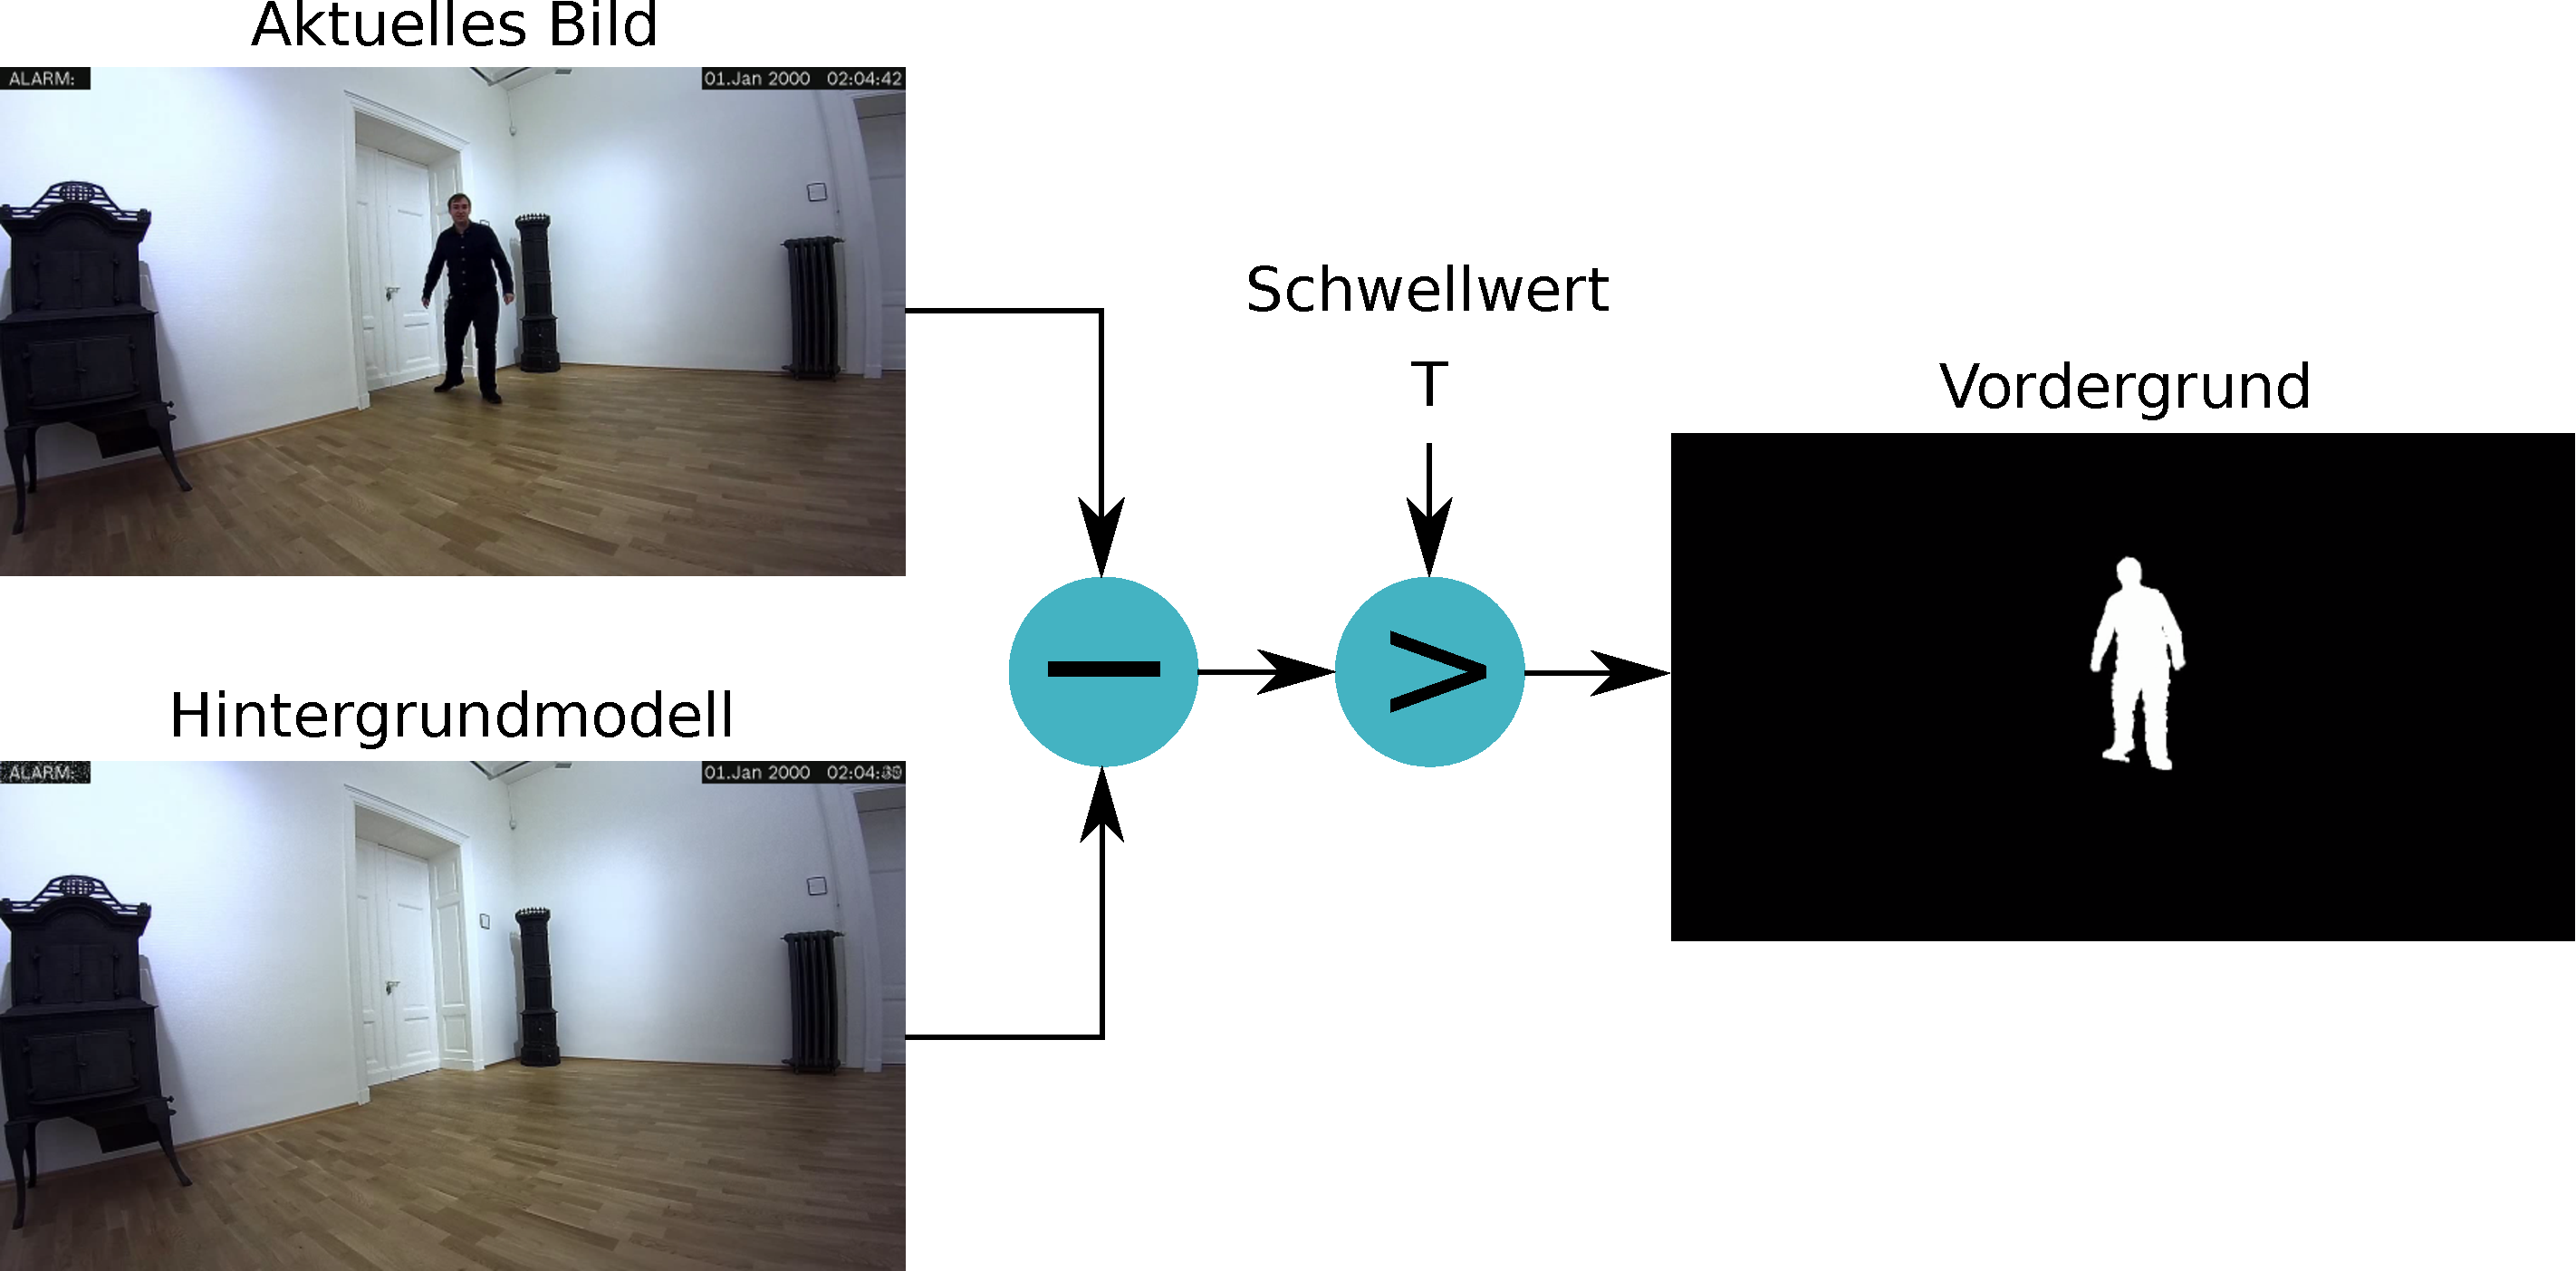
\includegraphics[width=1\textwidth]{fig/BS_Example.pdf}
	\caption{Ein Beispiel f�r die Hintergrundsubtraktion. }
	\label{fig:BS_Example}
\end{figure}
Im n�chsten Teil werden die Techniken beschrieben, die �berlicherweise  eingesetzt werden um eine Hintergrundsubtraktion durchzuf�hren.
\subsection{Adaptive Gaussian Mixture Model (AGMM)}
Die wissenschaftliche Arbeit \cite{kaewtrakulpong2002improved} entwickelte ein Hintergrundmodell auf Grundlage der Gau�schen Mischung. Diese Methode ist ein g�ngiges Verfahren zur Hintergrundsubtraktion. Es verwendet eine selektive Aktualisierungsmethode, um jedes Hintergrundpixel durch eine Mischung von K-Gau�schen Verteilungen (�blicherweise f�r K = 3 oder K = 5) zu modellieren \cite{kaewtrakulpong2002improved}. Verschiedene Gau�-Mischungen stellen die verschiedenen Farben dar. Die Gewichte der Gau�-Mischung repr�sentieren die Zeitanteile einer Farbe in der Szene. Die Pixel, die l�nger unver�ndert bleiben, sind die wahrscheinlichen Hintergrundfarben. F�r jedes neue Pixel wird anhand der bekannten Modellkomponenten �berpr�ft, ob der Pixelwert eine Hintergrundfarbe darstellt. Das Hintergrundmodell wird dann aktualisiert, wenn das Pixel in eine der K-Gau�schen-Komponenten passt. Aktualisierst wird nur die Erste passende K-Gau�sche-Komponente.  Wenn keine passende K-Gau�schen-Komponenten gefunden werden, wird eine neue Komponente mit dem Pixelwert als Mittelwert gesetzt, eine gro�e Kovarianz-Matrix und ein kleines Gewicht $w_k$ hinzugef�gt. \\
Jedes Pixel in der Szene wird durch eine Mischung von K-Gau�schen Verteilungen modelliert. Die Wahrscheinlichkeit, dass ein bestimmtes Pixel zum Zeitpunkt $n$ einen Wert von $\mathrm{x}_{n}$ hat, kann wie folgt beschrieben werden\cite{kaewtrakulpong2002improved}:\\
\begin{equation}
p(\mathrm{x}_{n}) = \sum \limits_{j=1}^K w_j \eta(x;\mu_k, \Sigma_k)
\end{equation}
wobei $w_j$ der Gewichtsparameter der k-ten Gau�-Komponente ist. Au�erdem ist $\eta(x;\mu_k, \Sigma_k)$ die Normalverteilung der k-ten Komponente, die wie folgt dargestellt wird \cite{kaewtrakulpong2002improved}:\\
\begin{equation}
\eta(x;\mu_k, \Sigma_k) = \frac{1}{(2\pi)^\frac{D}{2} |\Sigma_k|^\frac{1}{2}} \mathrm{e}^{-\frac{1}{2}(x-\mu_k)^T \Sigma_k^{-1}(x-\mu_k)}
\end{equation}
wobei $\mu_k$ der Mittelwert ist. Au�erdem ist $\Sigma_k =  \sigma^2_k I$ die Kovarianz der k-ten Komponente \cite{kaewtrakulpong2002improved}. Die K-Verteilungen sind auf der Grundlage des Fitnesswerts $\frac{w_k}{\sigma_k}$ geordnet und die ersten $B$-Verteilungen werden als ein Modell des Hintergrundes der Szene verwendet, wo $B$ wie folgt beschrieben wird\cite{kaewtrakulpong2002improved}:\\
\begin{equation}
B = \underset{b}{\arg\min}(\sum \limits_{j=1}^b w_j > T) 
\end{equation}
Der Schwellenwert $T$ ist der Mindestanteil des Hintergrundmodells und stellt die kleinste Wahrscheinlichkeit dar, dass der Hintergrund in der Szene bleibt. Die Hintergrundsubtraktion in \cite{kaewtrakulpong2002improved} wird durchgef�hrt, indem die Vordergrundpixel die Pixel sind, die in einer der B-Verteilungen eine Standardabweichung von mehr als $2,5$ aufweisen. Diese Pixel werden wei� gef�rbt. Die erste Gau�schen-Komponente, die die Bedingung 2.3 erf�llt, wird durch die folgenden Aktualisierungsgleichungen aktualisiert \cite{kaewtrakulpong2002improved}:
\begin{eqnarray}
\hat{w}^{N+1}_k &=& (1-\alpha) \hat{w}^{N}_k + \alpha \hat{p} (\Theta_k | \mathrm{x}_{N+1}) \\
\hat{\mu}^{N+1}_k &=& (1-\alpha) \hat{\mu}^N_k + \rho\mathrm{x}_{N+1} \\
\hat{\Sigma}^{N+1}_k &=& (1-\alpha)\hat{\Sigma}^N_k + \rho(\mathrm{x}_{N+1} - \hat{\mu}^{N+1}_k)(\mathrm{x}_{N+1} - \hat{\mu}^{N+1}_k)^T\\
\rho &=& \alpha\eta(\mathrm{x}_{N+1};\hat{\mu}^N_k; \hat{\Sigma}^N_k)\\
 \hat{p} (\Theta_k | x_{N+1})&=&\left\{\begin{array}{@{}ll@{}}
0, & \text{wenn}\ \Theta_k\ \text{erste passende Gau�-Komponente ist} \\
1, & \text{sonst}
\end{array}\right.
\end{eqnarray}
wobei $\Theta_k$ die k-te Gau�schen Komponente ist und $\frac{1}{\alpha}$ definiert die Zeitkonstante, die die �nderung bestimmt. Der aktualisierte Gewichtsparameter wird mit $\hat{w}^{N+1}_k$ genannt und $\hat{\mu}^{N+1}_k$, $\hat{\Sigma}^{N+1}_k$ sind erneute Mittelwert und Kovarianz.
Wenn keine der K-Verteilungen mit diesem Pixelwert zusammenpasst, wird die unwahrscheinliche Komponente durch eine Verteilung mit dem aktuellen Wert als Mittelwert, einer gro�en Kovarianz-Matrix und einem kleinen Gewicht ersetzt \cite{kaewtrakulpong2002improved}.
\subsection{Kernel Density Estimation (KDE)}
Ein Nachteil von \acs{AGMM} ist: Dieses Modell kann keine empfindliche Detektion erreichen, wenn der Hintergrund sehr hohe Frequenzvariation aufweist. Dieser Nachteil kann mit einem \acs{KDE} Modell, das in \cite{elgammal2000non} beschrieben wurde, gel�st werden.\\
Sei $x_1, x_2,..., x_n$ eine aktuelle Stichprobe von Intensit�tswerten f�r ein Pixel. Unter Verwendung dieser Stichprobe kann die Dichtefunktion der Wahrscheinlichkeit, dass dieses Pixel einen Intensit�tswert $x_t$ in Zeit $t$ hat, unter Verwendung des Kernsch�tzers $K$ mit Brandbreite $D$ als nicht-parametrisch gesch�tzt werden \cite{elgammal2000non}.
\begin{equation}
P(x_t) = \frac{1}{n} \sum \limits_{i=1}^n K_D (x_t - x_i) 
\end{equation}
Angenommen ist $D$ die Kernel-Funktionsbandbreite und verschiedene Farbkan�le werden mit unterschiedlichen Kernel-Bandbreiten $\sigma^2_j$ f�r den j-ten Farbkanal wie die Gleichung 2.10 dargestellt.

\begin{gather}
D
=
\begin{pmatrix}
\sigma^2_1 & 0 & 0 \\
0 & \sigma^2_2 & 0 \\
0 & 0 & \sigma^2_3 \\
\end{pmatrix}
\end{gather}
Wenn die Kernel-Sch�tzfunktion $K$ als Normalfunktion $N (0;\sigma)$ gew�hlt wird, wird die Dichtefunktion dann wie folgt beschrieben:
\begin{equation}
P(x_t) = \frac{1}{n} \sum \limits_{i=1}^N \prod \limits_{j=1}^d \frac{1}{\sqrt{2\pi\sigma^2_j}} \mathrm{e} ^ {-\frac{1}{2} \frac{({x_t}_j - {x_i}_j)^2}{\sigma^2_j}}
\end{equation}
Bei  $P(x_t)<T$ wird das Pixel als ein Vordergrundpixel betrachtet. In diesem Fall ist $T$ ein globaler Schwellenwert �ber das gesamte Bild. $T$ kann so eingestellt werden, dass nur ein minimaler Prozentsatz von fehlerhaften Erkennungen erreicht wird.\\
Angenommen ist $m$ Median von $|x_i - x_{i+1}|$ f�r jedes Paar $(x_i, x_{i+1})$ in der Stichprobe. Nach \cite{elgammal2000non} wird die Standardabweichung der ersten Verteilung wie folgt gesch�tzt: 
\begin{equation}
D = \frac{m}{0,68 \sqrt{2}}
\end{equation}
Bei \acs{KDE} gibt es zwei Alternativen f�r die Aktualisierung des Hintergrundes: \glqq{}Selective Update\grqq{} und \glqq{}Blind Update\grqq{}. Die erste Alternative f�gt neue Stichproben zum Modell hinzu, wenn sie als Hintergrund klassifiziert sind. Die zweite Alternative f�gt einfach neue Stichproben zum Modell hinzu, egal ob sie zum Hintergrund oder Vordergrund geh�ren. Im Allgemeinen funktioniert \acs{KDE} drau�en besser als die \acs{GMM} Methode.

\subsection{K-n�chster Nachbar (KNN)}
Diese Methode ist eine Verbesserung der \acs{KDE} Methode und wird in \cite{zivkovic2006efficient} als K-NN bezeichnet. Bei dieser Methode wird  die feste Kerngr��e $D$ in \acs{KDE} f�r jeden neuen Punkt $x_i$ angepasst. Anstatt der Optimierungen der Kerngr��e $D$, erh�ht diese Methode die Kerngr��en $D$, solang eine feste Menge von Daten $k$ abgedeckt ist. 
Mit der K-NN-Methode befinden sich gro�e Kerne in den Gebieten mit einer kleinen Anzahl von Stichproben und kleinere Kerne in den dicht besiedelten Gebieten. In ~\cite{zivkovic2006efficient} wird $k = [0.1n]$ gew�hlt, wobei $n$ die Zeit f�r die Anpassung des Modells ist und $[n]$ f�r das Aufrunden einer realen Zahl $n$ auf die n�chste nat�rliche Zahl steht. Ein neues Pixel $x_i$ passt zum Modell, wenn mehr als $k$ Punkte innerhalb von $n$ Kernen vorhanden sind. Aus diesem Grund wird der $k$-te Nachbar als Schwellenwert f�r diese Verbesserung verwendet. 

\subsection{Vibe}
In \cite{barnich2009vibe} wird ein Verfahren beschrieben, welches eine zuf�llige Aggregation der Hintergrundsubtraktion verwendet. Das Verfahren wird \glqq{}ViBe\grqq{} genannt. Sei $p_t(x)$ ein Pixelwert $x$ zur Zeit $t$. Beim \acs{GMM}- oder \acs{KDE}-Modell wird ein Pixelwert $p_t(x)$ als Hinter- oder Vordergrund klassifiziert, abh�ngig davon, wie des Pixel mit der Dichtefunktion des Modells passt. In \glqq{}ViBe\grqq{} wird eine Menge von Stichprobenwerten als Pixelmodell verwendet. Um einen Wert $p_t(x)$ zu klassifizieren, wird der Wert mit seinen n�chstliegenden Werten in der Menge der Stichproben verglichen, indem eine Kugel $S_R(p_t(x))$ mit Radius $R$ und Punkt $p_t(x)$ definiert wird. Ein Pixel ist genau dann als Hintergrund klassifiziert, wenn die �berschneidung $\sharp$ von der Kugel $S_R(p_t(x))$ und die Menge von Punkten ${p_1, p_2, ..., p_n}$ mehr als der Schwellenwert $\sharp_{min}$ ist (siehe Abbildung ~\ref{fig:vibe}).
\begin{figure}[h]
	\centering
	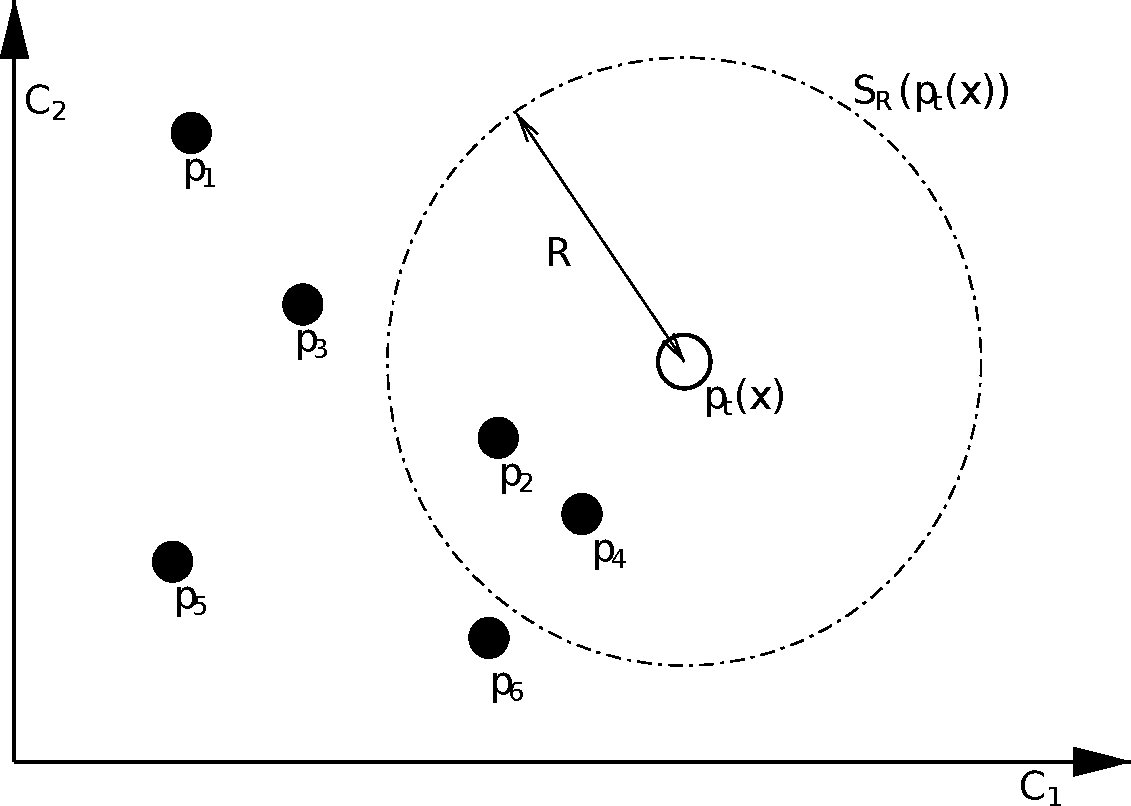
\includegraphics[width=0.5\textwidth]{fig/vibe.pdf}
	\caption{Die Klassifizierung von $p_t(x)$ basiert auf die �berschneidung der Kugel $S_R(p_t(x))$ mit der Menge der Stichproben \cite{barnich2009vibe}.}
	\label{fig:vibe}
\end{figure}
Im n�chsten Kapitel wird ein Vergleich der vier oben genannten Verfahren und meine eigene Methode beschrieben. Es wird auch auf die verschiedenen Vor- und Nachteile eingegangen.
\section{Histogrammanalyse}\label{sec:Histogrammanalyse}
Ein Histogramm eines Bilds stellt die Tonwertverteilung in einem digitalen Bild graphisch dar. Ein Bildhistogramm zeichnet die Anzahl der Pixel f�r jeden Tonwert auf. Es bietet ein n�tzliches Werkzeug f�r die $Schwellwertbildung$ auf dem Gebiet der Computervision an. Die graphische Darstellung von Histogrammen enth�lt Informationen �ber die Pixelverteilung als eine Funktion der Tonvariation, deswegen lassen sich Bild-Histogramme auf Hoch- und Tiefpunkte analysieren \cite{suttonhistograms}.\\ 
Jede K�rperhaltung erzeugt ein unterschiedliches Muster von Histogrammen, deswegen kann das Projektions-Histogramm als eins der Eigenschaften verwendet werden, um unterschiedliche K�rperhaltung zu unterscheiden. Nach der Hintergrundsubtraktion wird eine Silhouette des Vordergrundes als Bin�rbild erstellt. Eine K�rperhaltungsanalyse wird auf die Silhouette angewendet, um die �hnlichkeiten der horizontalen und vertikalen Projektions-Histogramme der erkannten Silhouette und der Haupthaltungen (Stehen, Beugen, Liegen und Sitzen) zu berechnen. Die Normalisierung des durchschnittlichen Histogramms erfolgt durch die Skalierung auf 128 Pixel der Silhouette indem sowohl H�he und Breite skaliert werden, bis beide Gr��en kleiner oder gleich 128 Pixel aufweisen. Dabei wird das urspr�nglichen Seitenverh�ltnis nicht ver�ndert. \cite{haritaoglu1998ghost}. Normalisierte horizontale und vertikale Referenz-Histogramme f�r jede K�rperhalterung wurden experimentell unter Verwendung von $4500$ Silhouetten von $7$ verschiedenen Personen berechnet \cite{haritaoglu1998ghost} (siehe Abbildung ~\ref{fig:histogramm}).   
\begin{figure}[h]
	\centering
	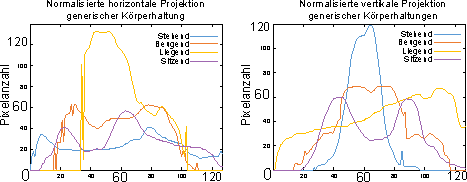
\includegraphics[width=1\textwidth]{fig/histogramm.pdf}
	\caption{Normalisierte horizontale und vertikale Referenz-Histogramme f�r jede K�rperhaltung \cite{haritaoglu1998ghost}.}
	\label{fig:histogramm}
\end{figure}
Die durch die Hintergrundsubtraktion erstellte Silhouette wird mit den durchschnittlichen Projektions-Histogrammen verglichen, wobei die Summe der absoluten Differenzen verwendet wird, um die �hnlichste K�rperhaltung zu ermitteln. Angenommen $S_i$ ist die �hnlichkeit zwischen der erkannten Silhouette und der i-ten K�rperhaltung. Seien $H_i$ und $V_i$ die horizontalen und vertikalen durchschnittlichen Projektions-Histogramme. $P$ und $R$ sind die horizontalen und vertikalen Histogramme der erkannten Silhouette. $S_i$ wird dann wie folgt berechnet: 
\begin{equation}\label{eq:loglikelyhood}
S_i = -\log(\sum \limits_{h}^{128} \sum \limits_{v}^{128} |H_h^i - P_h| + |V_v^i - R_v|) 
\end{equation}
Die K�rperhaltung, die das h�chste �hnlichkeitsma� ergibt, wird als die wahrscheinlichste Haltung angenommen.
\section{Fuzzylogik}\label{sec:fuzzylogik}
Unter Verwendung der Hintergrundsubtraktion zusammen mit einer Histogrammanalyse kann eine bewegte Person erkannt bzw. auch ihre K�rperhaltung ermittelt werden. . Um aus diesen gewonnenen Informationen eine au�ergew�hnliche Situationen zu erkennen, kommt die Fuzzylogik zum Einsatz. Im Jahre 1971  wurden die ersten Arbeiten �ber die sogenannte Fuzzy-Algebra ver�ffentlicht\cite{rosenfeld1971fuzzy}.\\
Es gibt mehre Gr�nde f�r den Einsatz der Fuzzylogik. Einer der Gr�nde ist, dass die mathematischen Konzepte hinter der Fuzzylogik einen geringen Grad an Komplexit�t haben.\\
Bei der Fuzzylogik geht es um viele frei w�hlbare Mengen, die jeweils einen Eingabeparameter abbilden. Die Mengen werden unter der gew�hlten Fuzzylogik definierten Regeln gerechnet. Durch die verschiedenen Kombinationen entstehen neue Mengen, die Fuzzymengen genannt werden.
Bei einer Kombination hei�t der Anteil des neuen Werts in einer Fuzzymenge, Mitgliedschaft-Grad. Der Mitgliedschaft-Grad beschreibt den Anteil des Eingabeparameters in einer Fuzzymenge.
Objekte bekommen den Wert $1$ zugewiesen, wenn sie vollst�ndig innerhalb der Fuzzymenge liegen. Objekten au�erhalb der Fuzzymenge bekommen den Wert $0$ zugewiesen. Jedes Objekt, das teilweise in der Menge ist, bekommt einen Wert aus dem offenen Intervall $(0, 1)$ zugewiesen. Der Prozess der Fuzzylogik wird wie folgt definiert ~\cite{dingle2011artificial}:
\begin{itemize}
\item Zuerst wird eine scharfe Menge von Eingabedaten gesammelt und unter Verwendung von Zugeh�rigkeit-Funktionen in Fuzzymengen umgewandelt. In diesem Schritt wird ein Zuordnung zwischen jedem scharfen Wert der Eingaben und der Fuzzy-Menge wie folgt erstellt \cite{cingolanijfuzzylogic}:\\
$A' = F(x_0)$\\
wobei $x_0$ ein scharfer Wert der Eingabe ist. $A'$ ist die Fuzzymenge der Mitgliederfunktion $F$. $F$ kann eine beliebige stetig Funktion wie z.B.: Eine Sinus-, Kosinus-, Sigmoid-, Gau�schen-Funktion sein. 
\item  Eine Schlussfolgerung wird basierend auf einer oder mehreren ($IF-THEN$) Regeln getroffen und die Regeln werden wie folgt beschrieben:\\
\textit{If X is A then Y is B}\\
\textit{Und wenn X A' ist, ergibt sich Y ist B'}\\
Wobei $X$ und $Y$ linguistische Variablen (Siehe Algorithmus \ref{algo:fuzzy}) sind. $A$ und $B$ sind Fuzzymengen, $B'$ ist die Ausgabe der Fuzzymenge. In diesem Schritt erh�lt das Fuzzysystem zun�chst den �bereinstimmungsgrad jeder Regel durch Anwendung eines konjunktiven Operators (AND- oder OR-Operator). Danach werden die Fuzzy-S�tze durch einen Fuzzy-Implikationsoperator (normalerweise Minimum oder Produkt) abgeleitet. Eine gleiche Anzahl von Ausgabes�tzen wie in den vordefinierten Regeln, werden an dieser Stelle erzeugt. Am Ende werden diese Gruppen von Ausgaben durch einen Aggregationsoperator (Maximum, Summe, normalisierte Summe, OR-Wahrscheinlichkeit) aggregiert. 
\item  Schlie�lich wird die Fuzzy-Ausgabe unter Verwendung der Zugeh�rigkeitsfunktionen in dem Defuzzifizierungsschritt auf eine scharfe Ausgabe abgebildet. Ein Wert f�r jede Variable wird mithilfe der ausgew�hlten Defuzzifizierungsmethode berechnet, die wie folgt definiert werden kann \cite{dingle2011artificial}:\\
\begin{itemize}
	\item Schwerpunkt: $\frac{\int x \mu (x) dx}{\int \mu (x) dx}$\\.
	\item Schwerpunkt Singleton: $\frac{\sum_{i}x_i\mu_i}{\sum_{i}\mu_i}$\\
	\item Zentrum der Region: $u|\int_{u}^{\infty} \mu(x) dx$\\
	\item Rightmost Maximum: $argmax_x [\mu (x) = max (\mu(x))]$\\
	\item Leftmost Maximum: $argmin_x [\mu (x) = max (\mu(x))]$\\
	\item Durchschnittliches Maximum: $mean(x) [\mu (x) = max (\mu(x))]$\\
\end{itemize}
\end{itemize}
Die Abbildung \ref{fig:Fuzzy_Example} stellt diese drei Schritte der Fuzzylogik in graphischen Bildern dar. Als Beispiel wird ein Thermostat genommen, dessen Ventil�ffnung entsprechend der Raumtemperatur gesteuert wird. Die hierzu erstellte Fuzzylogik bekommt die Temperatur als Eingabe und den �ffnungsgrad des Ventils als Ausgabe (siehe Abbildung \ref{fig:Fuzzy_Example}). Der Regel-Algorithmus wird wie in Algorithmus \ref{algo:fuzzy} definiert. Die Temperatur wird als \glqq{}Low, Medium und High\grqq{} klassifiziert. Wenn die Temperatur zwischen $0�$ und $20�$ ist, wird sie als \glqq{}Low\grqq{} klassifiziert. Werte zwischen $10�$ und $20�$ werden als \glqq{}Medium\grqq{} klassifiziert. Der Bereich von $20�$ bis $40�$ wird der Klassifizierung \glqq{}High\grqq{} zugeordnet. Als �ffnungsgrad des Thermotatventils wird das geschlossene Intervall $[1, 2]$ als \glqq{}Low\grqq{}, das Intervall $[1, 4]$ als \glqq{}Medium\grqq{} und letztlich das Intervall $[3, 5]$ als \glqq{}High\grqq{} klassifiziert. Eine Beispieleingabe der Temperatur von $23�$, die sich zwischen \glqq{}Medium\grqq{} und \glqq{}High\grqq{} befindet, ist in Abbildung \ref{fig:Fuzzy_Example} zu sehen. Bei $23�$ betr�gt der Mitgliedschaftsgrad $0.7$ zur Menge \glqq{}Medium\grqq{} und $0.3$ zu \glqq{}High\grqq{}. Nach der Regel in Algorithmus \ref{algo:fuzzy}, wird der �ffnungsgrad des Thermotatventils zwischen \glqq{}Low\grqq{} und \glqq{}Medium\grqq{} berechnet und mit der Methode \glqq{}Schwerpunkt\grqq{} liegt der �ffnungsgrad des Thermotatventils bei $2.15$.\\
\begin{figure}[H]
	\centering
	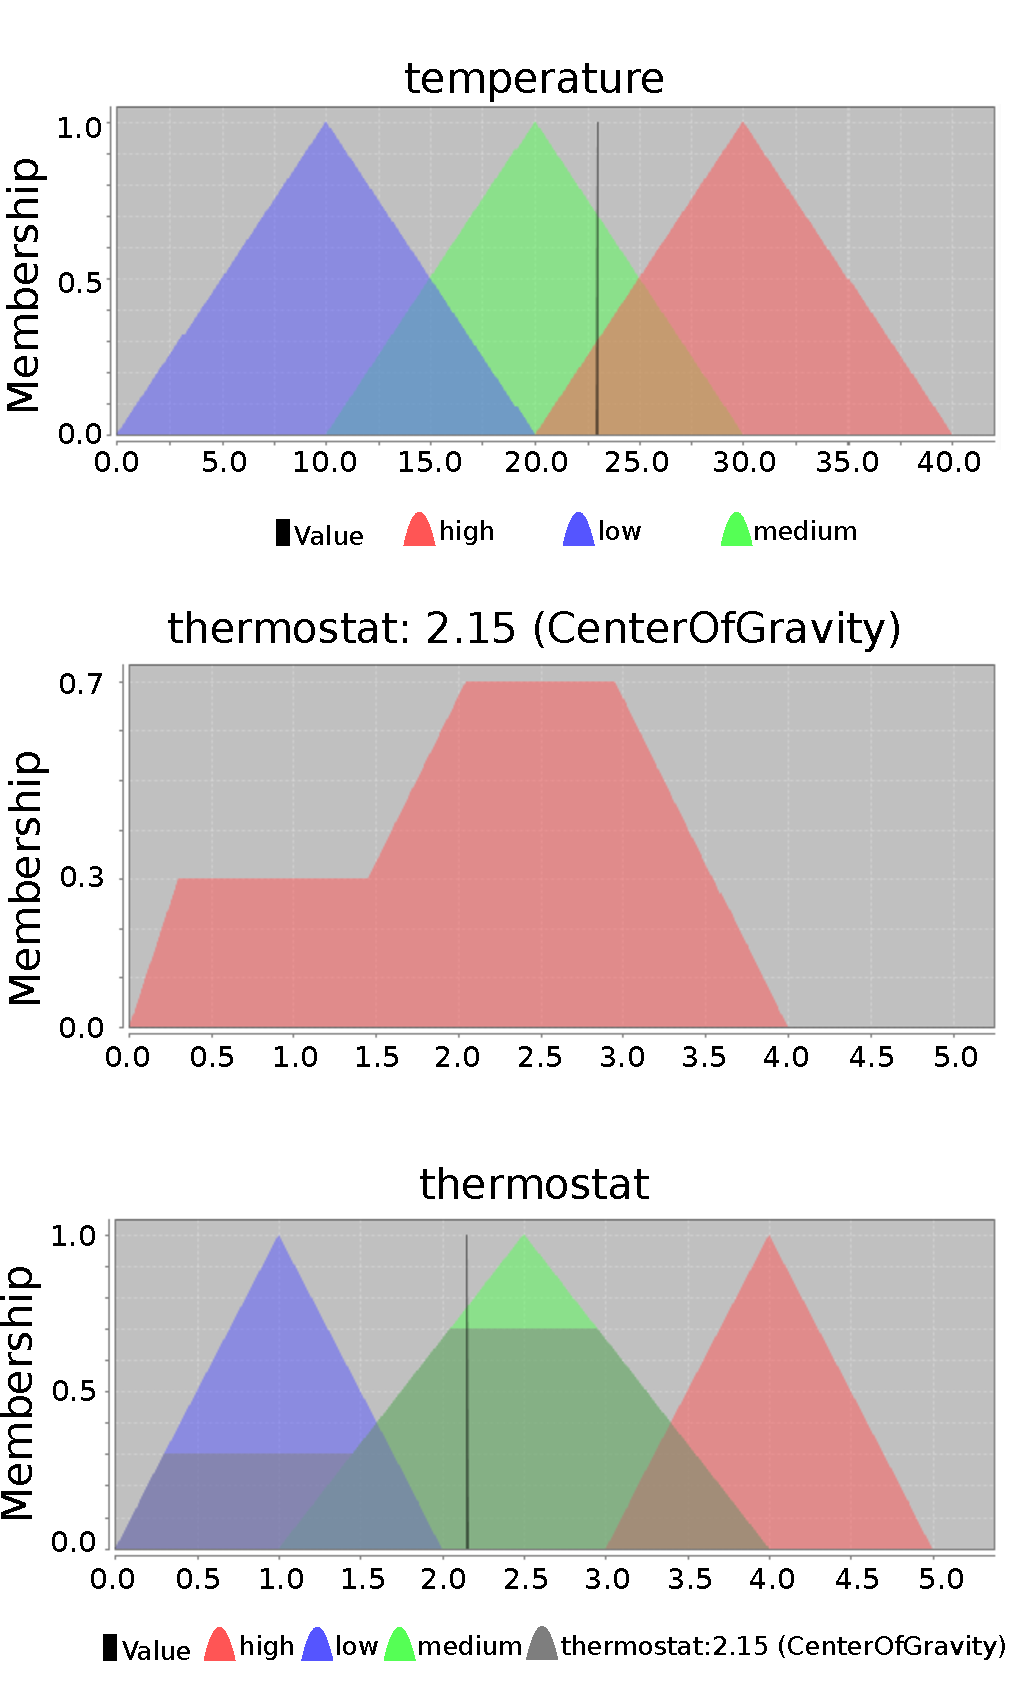
\includegraphics[width=0.59\textwidth]{fig/fuzzy.pdf}
	\caption{Ein Beispiel f�r die Fuzzylogik in drei Schritten. Oben: Die Temperatur von $23$ Grad wird durch Mitgliederfunktionen abgebildet. Mitte: Durch die (IF-ELSE) Regel in Algorithmus \ref{algo:fuzzy} wird eine Ausgabe als Fuzzymenge berechnet. Unten: Ein Schwerpunkt von der gerechneten Ausgabe wird in eine scharfe Ausgabe abgebildet und es ergibt sich der Wert 2.15 f�r das Thermostat.} 
	\label{fig:Fuzzy_Example}
\end{figure}
\begin{algorithm}[H]
\caption{Regel f�r Raumtemperatur und Einstellung des Thermostates.	}
\label{algo:fuzzy}
\If{temperature IS low}{thermostat IS high;}
\If{temperature IS medium}{thermostat IS medium;}
\If{temperature IS high}{thermostat IS low;}
\end{algorithm}
Die Berechnung und graphische Darstellung der Fuzzylogik in dieser Arbeit werden mit der Open-Source-Bibliothek \glqq{}jFuzzyLogic\grqq{} realisiert.
\section{OpenCV Framework}\label{sec:OpenCV}
OpenCV steht f�r Open-Computer-Vision. Die Bibliothek ist in C und C++ programmiert und kann auf vielen Betriebsystemen verwendet werden. OpenCV kann auch mithilfe von Java, Python, Ruby, Mathlab... verwendet werden. OpenCV wurde mit Fokus auf Recheneffizienz entwickelt, um Echtzeitanwendungen zu unterst�tzen. Diese Bibliothek enth�lt �ber 500 Funktionen, die viele Bereiche der Bildverarbeitung einschlie�lich maschinellem Lernen, neuronaler Netze, usw. umfassen\cite{bradski2008learning}. OpenCV vereinfacht den Bildverarbeitungsprozess mit vielen hilfreichen vordefinierten Funktionen. Da es sich in dieser Arbeit um ein Echtzeitanwendung handelt, wird auf OpenCV gesetzt, um die Verarbeitungszeit gering zu halten.

\section{360� Kamera}
Ziel dieser Arbeit war es, eine Echtzeitanwendung zu entwickeln die mit der Bosch Smart Home Innenkamera funktioniert. Die Testvideos in dieser Arbeit wurden mit dieser Kamera aufgenommen. Die Bosch 360� Innenkamera kann sich in jede Richtung (360�) drehen. Die Kamera verf�gt �ber Bewegungssensoren, eine Gegensprechanlage f�r Zwei-Wege-Audio und Infrarot-Nachtsicht-Funktion. Sie zeichnet Bild-Material in HD-Qualit�t auf. Das Bild-Material kann auf PC bzw. externen Speicher kopiert werden. Die Innenkamera verf�gt �ber verschiedene Schnittstellen wie zum Beispiel WLAN. Die Internetverbindung wird von der Kamera genutzt, um Push-Nachrichten an ein Smartphone zu schicken. Dank der integrierten Bewegungsmelder kann die Kamera einer Bewegung folgen bzw. sich automatisch drehen, um das bewegte Objekt im Bild zu halten. Dies ist in dieser Arbeit sehr hilfreich.
\begin{figure}[H]
	\centering
	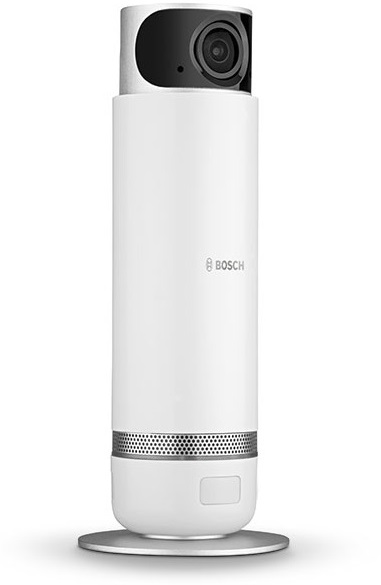
\includegraphics[width=0.5\textwidth]{fig/BoschInnenkamera.jpg}
	\caption{Bosch 360� Kamera (Quelle: www.bosch-smarthome.com) } 
	\label{fig:BoschInnenCam}
\end{figure}
\newpage
\newpage\thispagestyle{empty}\hspace{1em}\newpage
\chapter{Eigenes Verfahren}\label{chp:EigVerfahren}
Diese Arbeit besteht aus drei gro�e Meilensteine. Das Hintergrundsubtraktion-Verfahren, Sch�tzung der K�rperhaltung mithilfe von einer Histogrammanalyse und die Erkennung von au�ergew�hnlichen Situationen mithilfe der Fuzzylogik. Die Abbildung \ref{fig:allgemein} veranschaulicht die erw�hnten Meilensteine nochmals.\\
Die hier verwendeten Testvideos haben eine Aufl�sung von 1280x720 Pixel und werden mit 15 Frames pro Sekunde aufgenommen. Der erste Meilenstein besteht aus der Hintergrundsubtraktion, und wird in Blau dargestellt. Die Eingabe f�r eine Hintergrundsubtraktion ist ein von der Kamera aufgenommenes Bild und die Ausgabe ist eine Silhouette einer Person. Der zweite Meilenstein ist die Histogrammanalyse, die zur Erkennung einer K�rperhaltung zum Einsatz kommt, und ist der gelbe Teil der Abbildung . Die Eingabe dieses Meilensteins ist die Silhouette aus dem vorherigen Schritt und die Ausgabe ist die Sch�tzung der K�rperhaltung der Person auf der >Silhouette. Der letzte Meilenstein ist die Fuzzylogik, die mit der roten Farbe dargestellt ist. Die Eingaben der Fuzzylogik sind die Sch�tzung der K�rperhaltung, die Position der Person und die Zeit. Die Aufgabe der Fuzzylogik ist es, eine Entscheidung zu treffen, ob es sich um eine au�ergew�hnliche Situation handelt oder nicht.
\begin{figure}[H]			
	\centering
	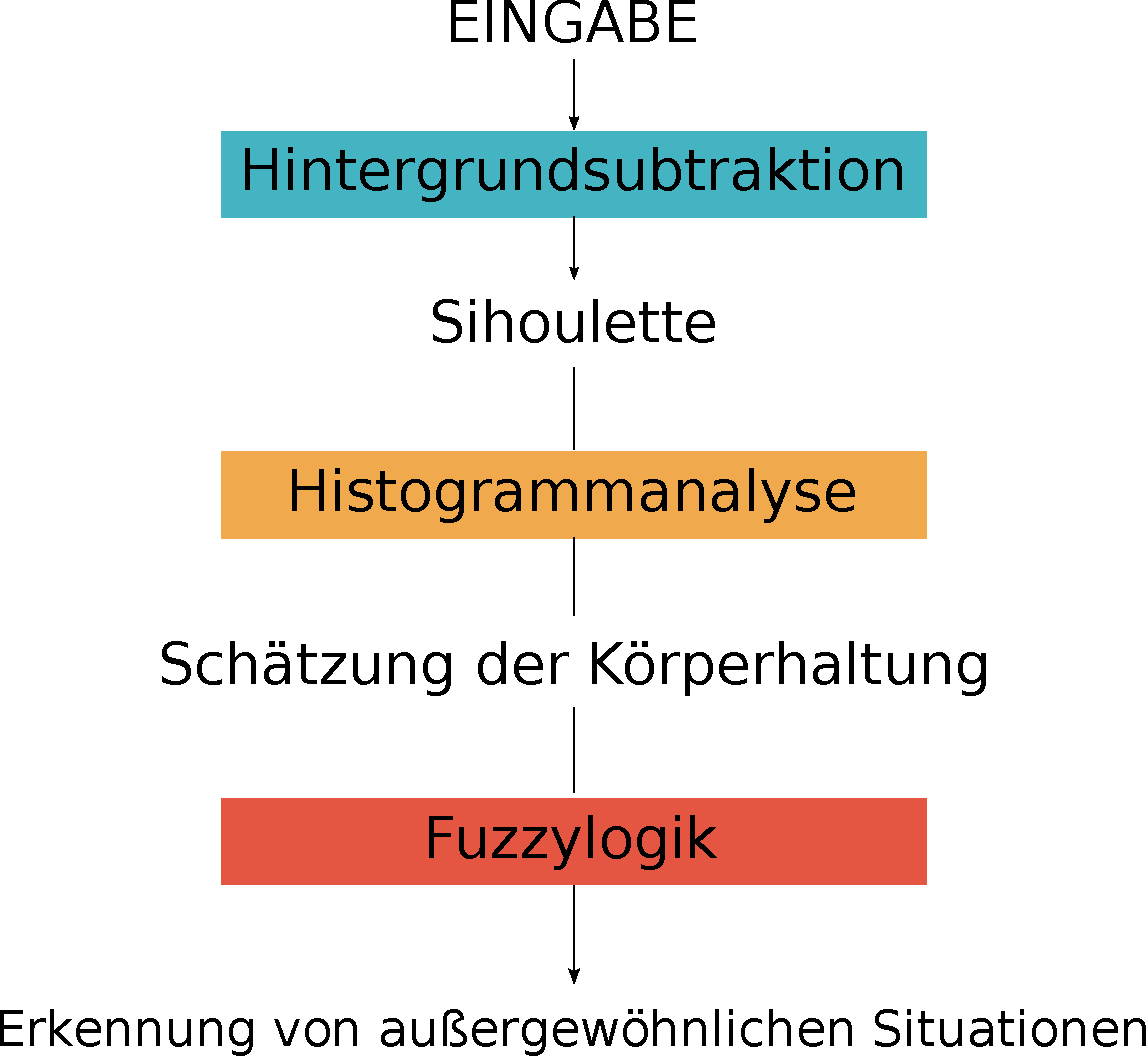
\includegraphics[width=0.65\textwidth]{fig/allgemein.pdf}
	\caption{Die drei Meilensteine zur Erkennung von au�ergew�hnlichen Situation.}
	\label{fig:allgemein}
\end{figure}

\section{Die Hintergrundsubtraktion}\label{chp:BackgroundSubtraction}
\subsection{Vergleich verschiedener Methoden}
Die Abbildung \ref{fig:bgsub} zeigt allgemein die Grundfunktion der Hintergrundsubtraktion. Die Aufgaben dieses Verfahrens ist es, von der Bildeingabe den statischen Teil des Bildes zu extrahieren bzw. den Hintergrund korrekt zu filtern und in ein Modell zu speisen. Au�erdem soll dieses Hintergrundmodell immer aktuell bleiben, so wird je Eingabe Frame/Bild das Hintergrundmodell aktualisiert.

\begin{figure}[H]
	\centering
	
\includegraphics[width=1\textwidth]{fig/bgsub.pdf}
	\caption{Veranschaulichung des Hintergrundsubtraktion-Verfahren.}
	\label{fig:bgsub}
\end{figure}
Es existieren mehrere Verfahren, um eine Hintergrundsubtraktion durchzuf�hren.
Um ein f�r diese Arbeit geeignetes Verfahren zu finden, wurden zuerst mehrere Verfahren verglichen.  Im Abschnitt \ref{sec:grunglagen_hintergrundsub} (Gaussian Mixture Model, K-n�chste Nachbar, Kernel Density Estimation und Vibe) wurden die bekanntesten Verfahren theoretisch beschrieben. Hier werden die einzelnen Verfahren so gepr�ft, um herauszufinden, ob sie f�r den Echtzeiteinsatz geeignet sind oder doch nicht. Die f�r diese Arbeit eingesetzte Kamera nimmt bis zu 15 Frames die Sekunde auf. Des weiteren betr�gt die hier verwendete Rechenleistung 13.75 GFlops. Ziel ist es, ein Verfahren auszuw�hlen, dass 15 Frames pro Sekunde mit der eingesetzten Rechenleistung abarbeiten kann. Die Rechenleistung gilt nicht als besonders Leistungsf�hig. Bei \acs{AGMM} wird eine Mischung von 5 Gau�schen Verteilungen f�r das Hintergrundmodell verwendet und die Historie des Hintergrundmodells auf 100 Bilder limitiert. Die Lernrate wird auf $0.01$ gesetzt. F�r das \acs{KNN} Verfahren wurden auch die Parameter mit den gleichen Werten belegt, um den Vergleich der Hintergrundsubtraktionsverfahren objektiv bewerten zu k�nnen. Bei \acs{KDE} handelt es sich um eine Berechnung von Intensit�tswerten f�r jeden Pixel, daher wird nur der Parameter der \grqq{}Historie\grqq{} (wie bei \acs{AGMM}) belegt. Wie in \cite{barnich2009vibe} beschrieben, ist Vibe ein nicht-parametrisches Verfahren, deshalb musste kein Parameter konfiguriert werden.
In der folgenden Abbildung werden die Vergleiche der vier Verfahren veranschaulicht.

\begin{table}[H]
	\begin{center}
		\begin{tabular}{ | c  | c  | }
			\hline
			\raisebox{-\totalheight}{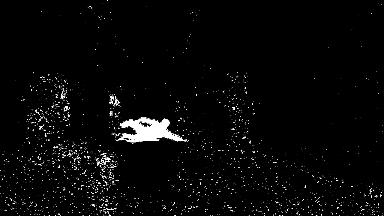
\includegraphics[width=0.5\textwidth]{fig/motiondetrection_AGMM.png}}
			& 
			\raisebox{-\totalheight}{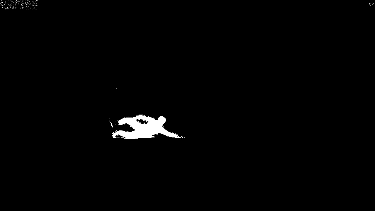
\includegraphics[width=0.5\textwidth]{fig/motiondetrection_KNN.png}}
			\\
			1. AGMM & 2. KNN\\
			\hline
			
			\raisebox{-\totalheight}{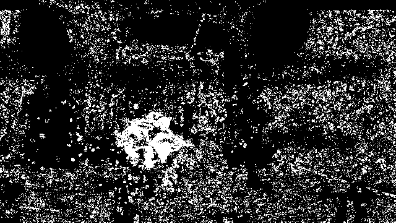
\includegraphics[width=0.5\textwidth]{fig/motiondetrection_KDE.png}}
			& 
			\raisebox{-\totalheight}{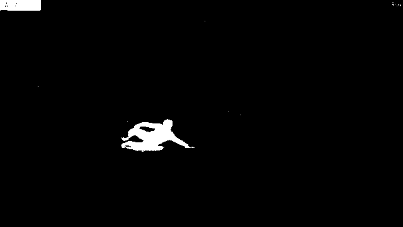
\includegraphics[width=0.5\textwidth]{fig/motiondetrection_Vibe.png}}
			\\
			3. KDE & 4. Vibe\\
			\hline
		\end{tabular}
		\caption{Vergleiche von 1. AGMM 2. KNN 3. KDE 4. Vibe}
		\label{fig:compare_bgsubtraction}
	\end{center}
\end{table}
Aus der obigen Grafik wird deutlich, dass sich in den Verfahren AGMM und KNN viel Rausch im Resultat der Hintergrundsubtraktion befindet. Die Resultate sind daher als schlecht zu bewerten. Die Verfahren KDE und Vibe liefern sehr gut Resultate bzw. eine Silhouette mit weniger Rausch, jedoch ben�tigt das Vibe-Verfahren deutlich mehr Zeit. Somit ist das Verfahren KNN, verglichen mit den anderen, das Verfahren, dass eine klare Silhouette mit weniger Rausch in k�rzester Zeit liefert. 
Anhand des Schaubildes ist das \acs{KNN}-Verfahren ein geeigneter Kandidat f�r die Echtzeitanwendung. Nun muss noch gepr�ft werden, ob sich das Verfahren f�r bis zu 15 Frames einsetzten l�sst. Aus dem Test war nur zu erkennen, dass es in erster Linie ein valides Resultat liefert. Zweitrangig wurden die Verfahren nach der Zeit bewertet. Aus dem Test ist nicht ganz ersichtlich, ob sich das Verfahren denn im Dauerbetrieb anwenden l�sst. Um das zu pr�fen, wurden viele Testvideos mit Tageslicht und andere abends mit h�uslicher Beleuchtung aufgenommen und analysiert. Ziel ist es, dass die Echtzeitanwendung stabile Resultate bei allen Beleuchtungen liefert.

Aus der Tabelle \ref{fig:compare_bgsubtraction} mit vier Abbildungen ist zu sehen, dass die Verfahren Vibe und KNN deutlich bessere (weniger Rauschen) Resultate liefern. Um aus den beiden Verfahren eins auszuw�hlen, wird eine Laufzeitanalyse bestimmt. Die Abbildung \ref{fig:vibeknn} stellt die Laufzeitanalyse der Verfahren KNN und Vibe mit einem Rechner, der mit einem Intel i5 3,20 GHz ausgestattet ist, dar.

\begin{figure}[H]
	\centering
	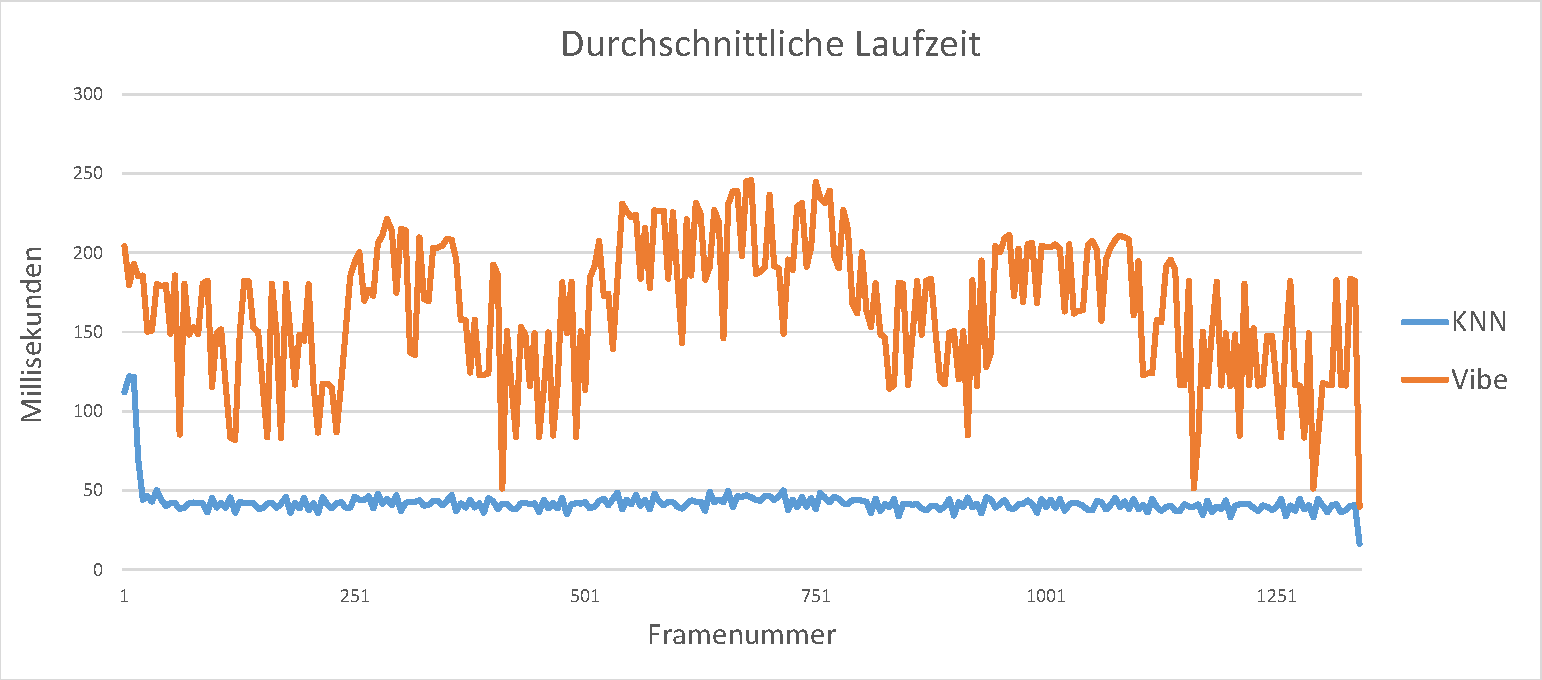
\includegraphics[width=1\textwidth]{fig/knn_vs_vibe_edit.pdf}
	\caption{Die Verarbeitungszeit von KNN und Vibe werden verglichen. Es ist deutlich, dass KNN eine k�rzere durchschnittliche Verarbeitungszeit (42ms) als Vibe (165ms) hat.} 
	\label{fig:vibeknn}
\end{figure}

Aus der obigen Laufzeitanalyse ist zu entnehmen, dass das KNN-Verfahren deutlich effizienter ist als das Vibe-Verfahren. Aus den Gr�nden, dass das KNN-Verfahren gute Resultate in Bestzeit im Vergleich liefert, wird f�r die Echtzeitanwendung dieser Arbeit auch dieses Verfahren eingesetzt. Die oben genannten Hintergrundsubtraktionsverfahren basieren auf der �nderung der Intensit�tswerten jedes Pixel, deshalb liefern die Verfahren ein Bin�rbild mit Rausch zur�ck. Um das Rauschen zu entfernen, kommen Erosion und Dilatation zum Einsatz. Die zwei Verfahren sind die grundlegenden Operationen bei der morphologischen Bildverarbeitung, auf der alle anderen morphologischen Operationen basieren. Um das Rauschen zu entfernen, wird das Verfahren �ffnung verwendet. Der Begriff �ffnung bedeutet eine Schachtelung von den Verfahren Erosion und Dilatation hintereinander.

Die Erosion ist ein Verfahren, dass ein Bild mit einem vordefinierten Filter untersucht und daraus Schlussfolgerungen zieht, wie dieser Filter in die Formen im Bild passt. Wenn ein Pixel und seine Nachbarpixel vollst�ndig von dem Filter �berlagert werden, wird das Pixel nicht ver�ndert, sonst wird das Pixel gel�scht. Gel�scht wird indem das Pixel schwarz wird. Angenommen ist $A$ ein Bin�rbild und $B$ ein Filter mit einem Zentrum in der Mittel von $B$. Wenn $B$ sich in $A$ bewegt, �berlagert f�r jedes Pixel in $A$ der Ursprung von $B$. Wenn $B$ vollst�ndig in $A$ enthalten ist, wird das Pixel bei der Erosion beibehalten, ansonsten gel�scht\cite{zamperoni2013methoden}. Die folgende Grafik veranschaulicht die Erosion.
\begin{figure}[H]
	\centering
	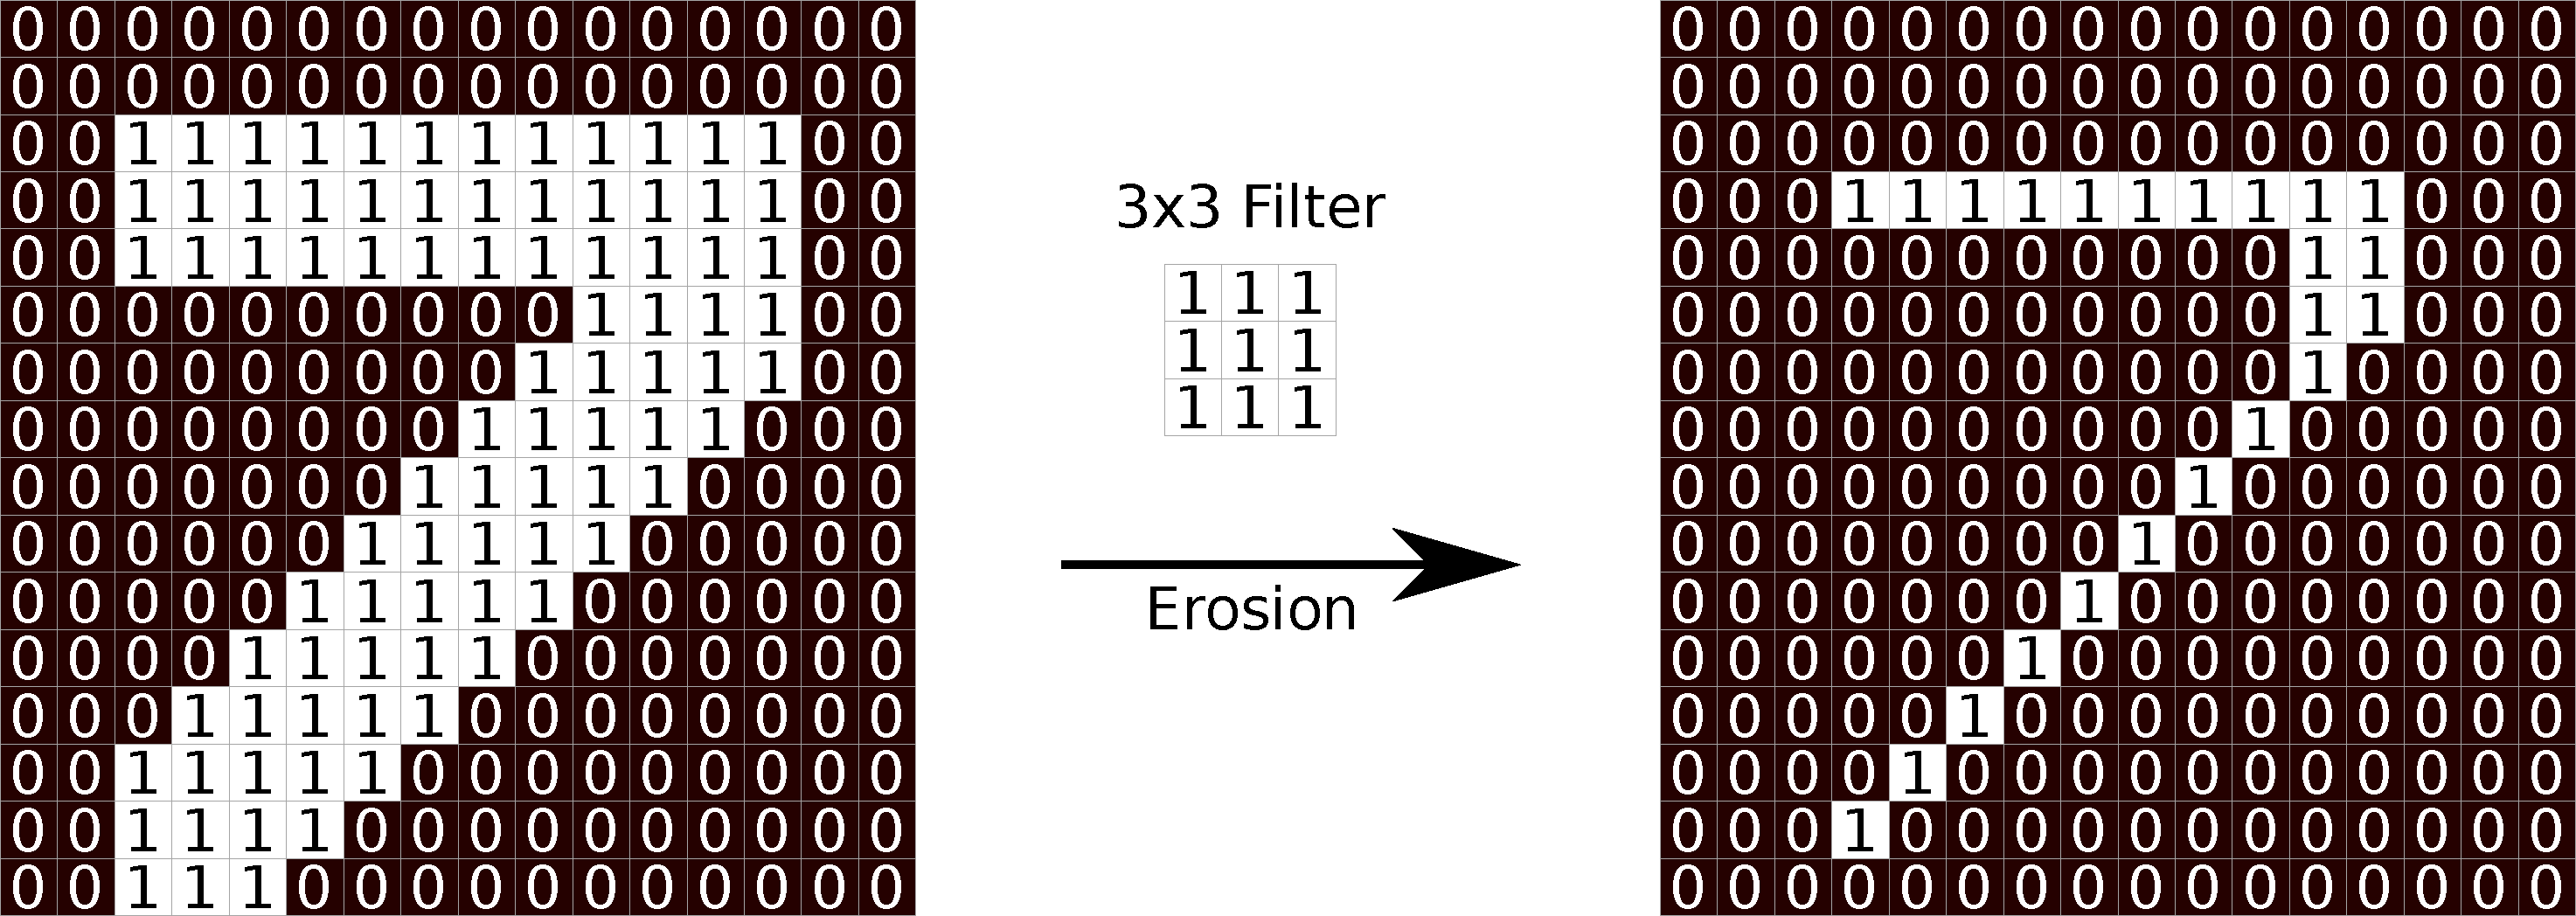
\includegraphics[width=0.8\textwidth]{fig/erosion.pdf}
	\caption{Die Erosion mit einem 3x3 Filter.} 
	\label{fig:erosion}
\end{figure}
Die Dilatation ist ein gegenteiliges Verfahren zur Erosion, es versucht die Form eines Bildes zu vergr��ern. Wenn $B$ sich in $A$ bewegt, �berlagert f�r jedes Pixel in $A$ der Ursprung von $B$. Alle Pixel in $A$, die vollst�ndig von $B$ �berlagert sind, werden beibehalten oder markiert \cite{zamperoni2013methoden}.\\
Die folgende Grafik veranschaulicht die Dilatation.
\begin{figure}[H]
	\centering
	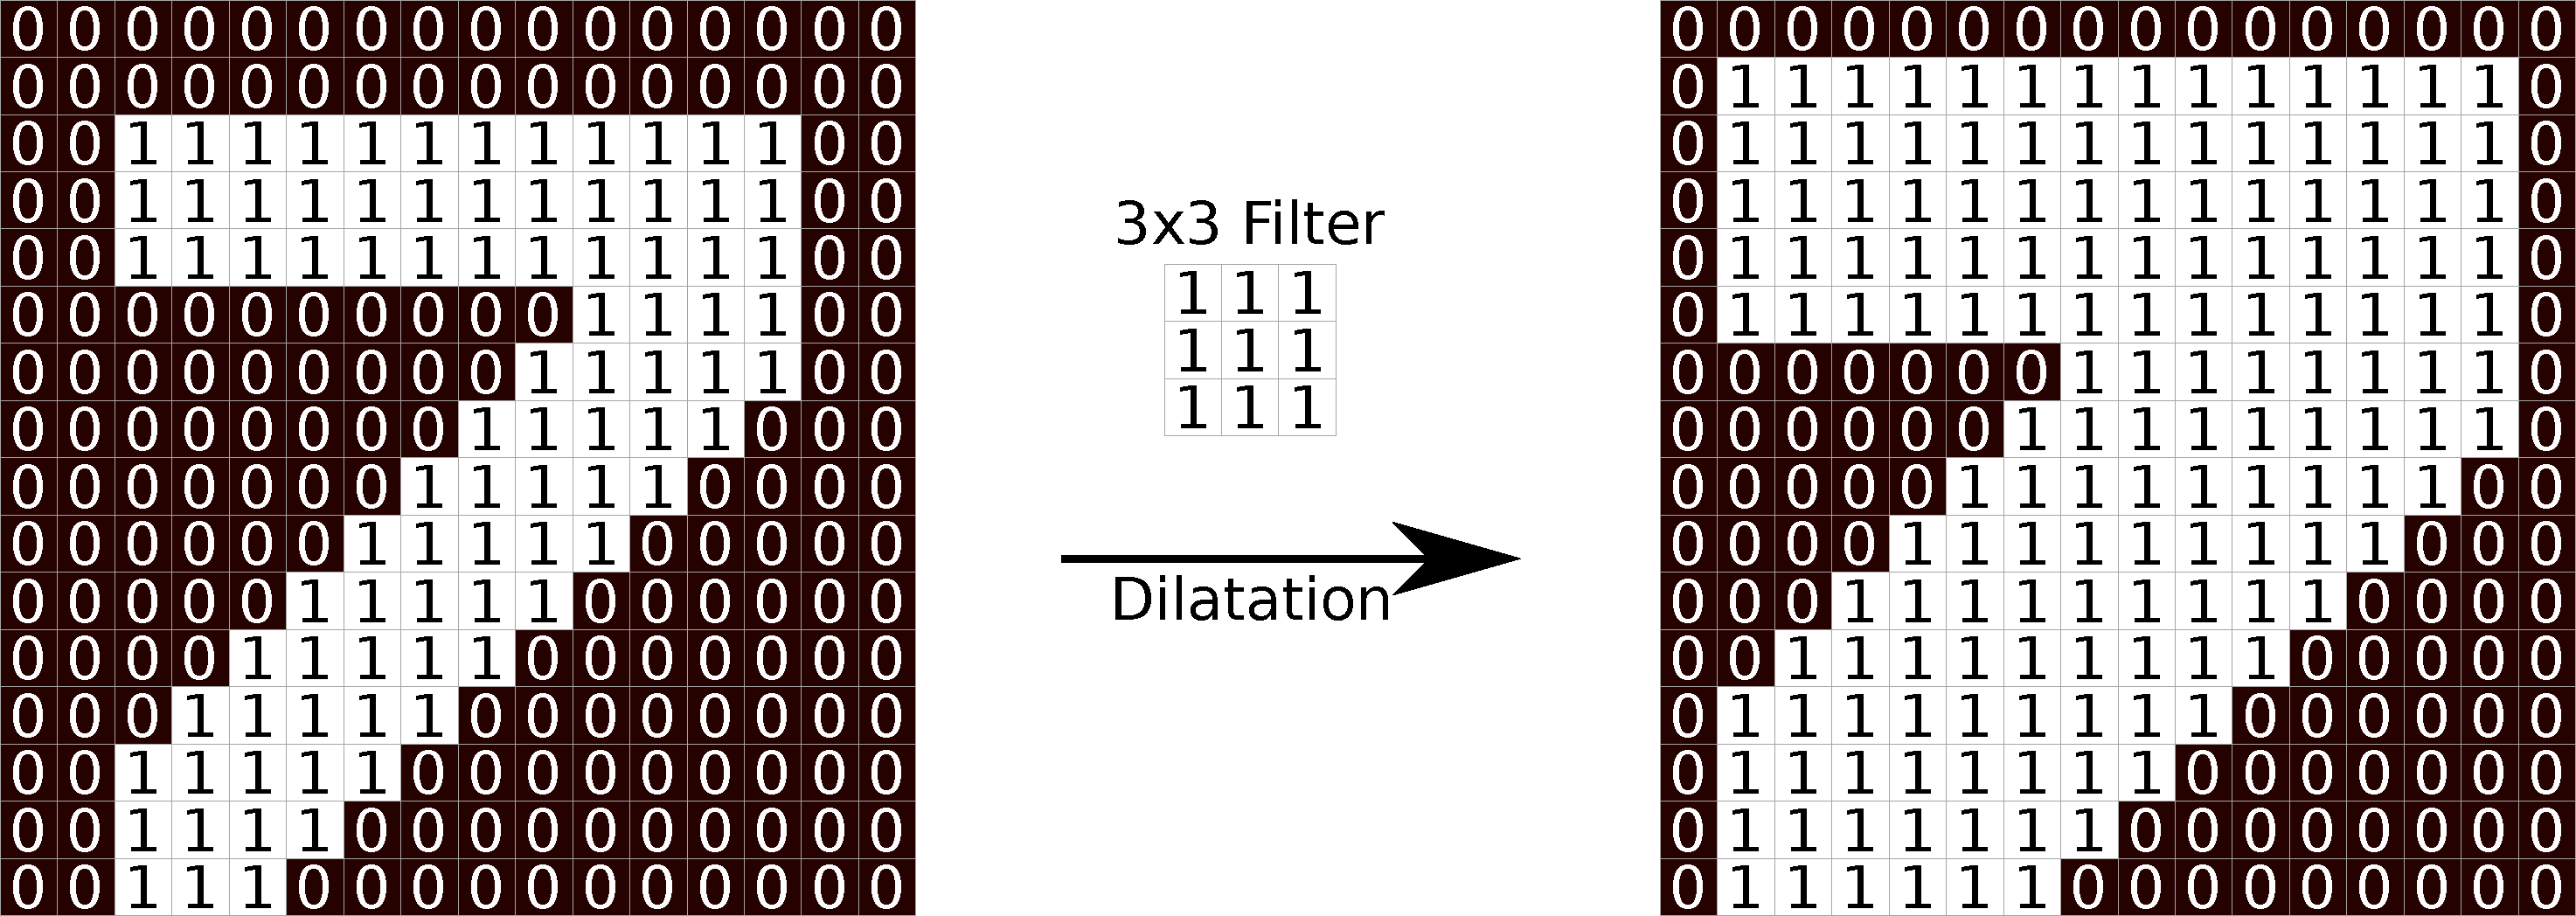
\includegraphics[width=0.8\textwidth]{fig/dilatation.pdf}
	\caption{Die Dilatation mit einem 3x3 Filter.} 
	\label{fig:dilatation}
\end{figure}
Um den Rausch aus der Silhouette zu entfernen wird das �ffnen-Verfahren angewandt. Auf die Silhouette wird zuerst eine Erosion durchgef�hrt und anschlie�end eine Dilatation. Durch diese Ma�nahme wird die Silhouette zuerst scharfer bzw. alle Punkte, die nicht zur Person auf der Silhouette geh�ren, gel�scht. Allerdings kann es passieren, dass die Punkte die zur Person geh�ren etwas undichter werden. Um diesen Fehler zu verbessern und die Silhouette wieder auf die original Gr��e zur�ck zu bekommen, wird die Dilatation angewendet. So bleibt am Ende die Silhouette gleich gro�e und ohne Rausch.\\
Die Abbildung \ref{fig:eroanddila} zeigt, dass nach Erosion unerwartetes Rauschen au�er Silhouette entfernt ist und auch die Silhouette kleiner wird. Um dies zu kompensieren wird eine Dilatation verwendet. 
\begin{figure}[H]
	\centering
	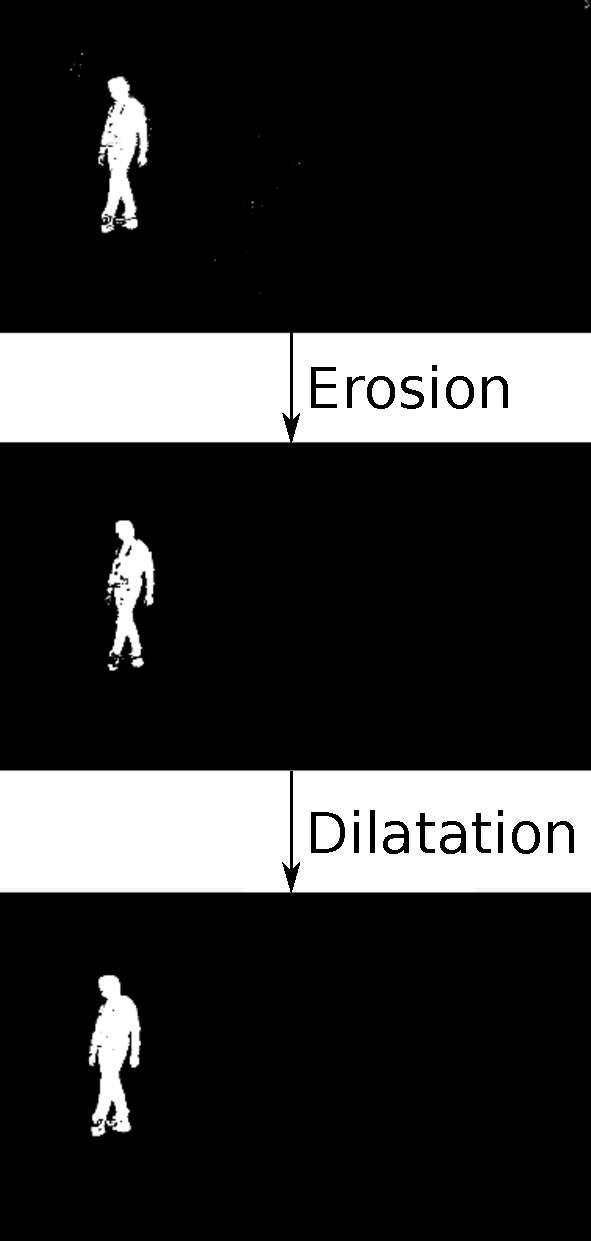
\includegraphics[width=0.6\textwidth]{fig/eroanddila.pdf}
	\caption{Ein Beispiel f�r die �ffnung (Erosion und Dilatation).}
	\label{fig:eroanddila}
\end{figure}
\subsection{Erweiterungen f�r die Hintergrundsubtraktion}
Im Allgemeinen wird f�r jedes Pixel des aktuellen Bilds geschaut, ob es dem Hintergrund zugeh�rig ist. Das funktioniert wie beschrieben sehr zuverl�ssig. Nun wird folgende Situation betrachtet: Eine Person befindet sich eine gewisse Zeit im Raum und bewegt sich nicht. Durch die st�ndige Aktualisierung des Hintergrundmodells wird die Person Fehlerhaft als Hintergrund erkannt und verschwindet in das Hintergrundmodell. So kommt die Aufgabe dieser Echtzeitanwendung nicht zum Einsatz, weil bei einer Au�ergew�hnlichen Situation muss sich eine Person eine gewisse Zeit nicht mehr bewegen bzw. auf dem Boden liegen. Aber dieser Fall wird nie auftreten. Auch Situationen wo die Person zum Beispiel auf dem Sofa liegt und TV sieht, befindet sich die Person nicht in Gefahr und auch nicht im Hintergrund. 
\subsubsection{Erste Verbesserung: Aktualisierung der selektiven Begrenzungsboxen}
Um das oben genannte Problem zu l�sen, wo eine sich nicht bewegende Person in das Hintergrundmodell integriert wird, obwohl die Person in den Vordergrund bleiben soll, wurde ein eigenes Verfahren entwickelt. Dieses Verfahren erstellt bei der Verarbeitung der Frames Begrenzungsboxen in Form von Rechtecken zur bewegten Person. Diese Begrenzungsboxen sind Minimal bzw. umh�llen die Person mit dem kleinst m�glichen Fl�chen. Das hei�t, auch wenn die Person sich lange nicht bewegt, bleibt sie ein Objekt, dass sich bewegt und wird nicht in das Hintergrundmodell integriert. Das geschieht durch eine gef�hrte Liste der Begrenzungsboxen. Diese Liste hat die gleiche L�nge wie die gesetzte Historie des Hintergrundsubtraktionsverfahren. So wird bei jedem zu verarbeitenden Frame eine Begrenzungsbox aus der Silhouette erstellt und mit der Liste aus vorherigen Begrenzungsboxen verglichen. Falls die neue Begrenzungsbox mit den vorherigen Begrenzungsboxen keine �berschneidungen hat, werden diese Begrenzungsboxen in das Hintergrundmodell hinzugef�gt und aus der Liste entfernt. Die neue Begrenzungsbox wird immer der Liste hinzugef�gt, egal ob es �berschneidungen gibt oder nicht. So k�nnen Personen die sich im Raum befinden und sich dann auf das Sofa legen und sich ausruhen, bleiben im Vordergrund bis sie die Szene verlassen. Wie das modifizierte Hintergrundsubtraktionsverfahren, genannt \glqq{}Aktualisierung der selektiven Begrenzungsboxen\grqq{} (ASB), arbeitet, zeigt folgende Grafiken \ref{fig:mymethod1}, \ref{fig:mymethod2}, \ref{fig:mymethod3}.
\begin{figure}[H]
	\centering
	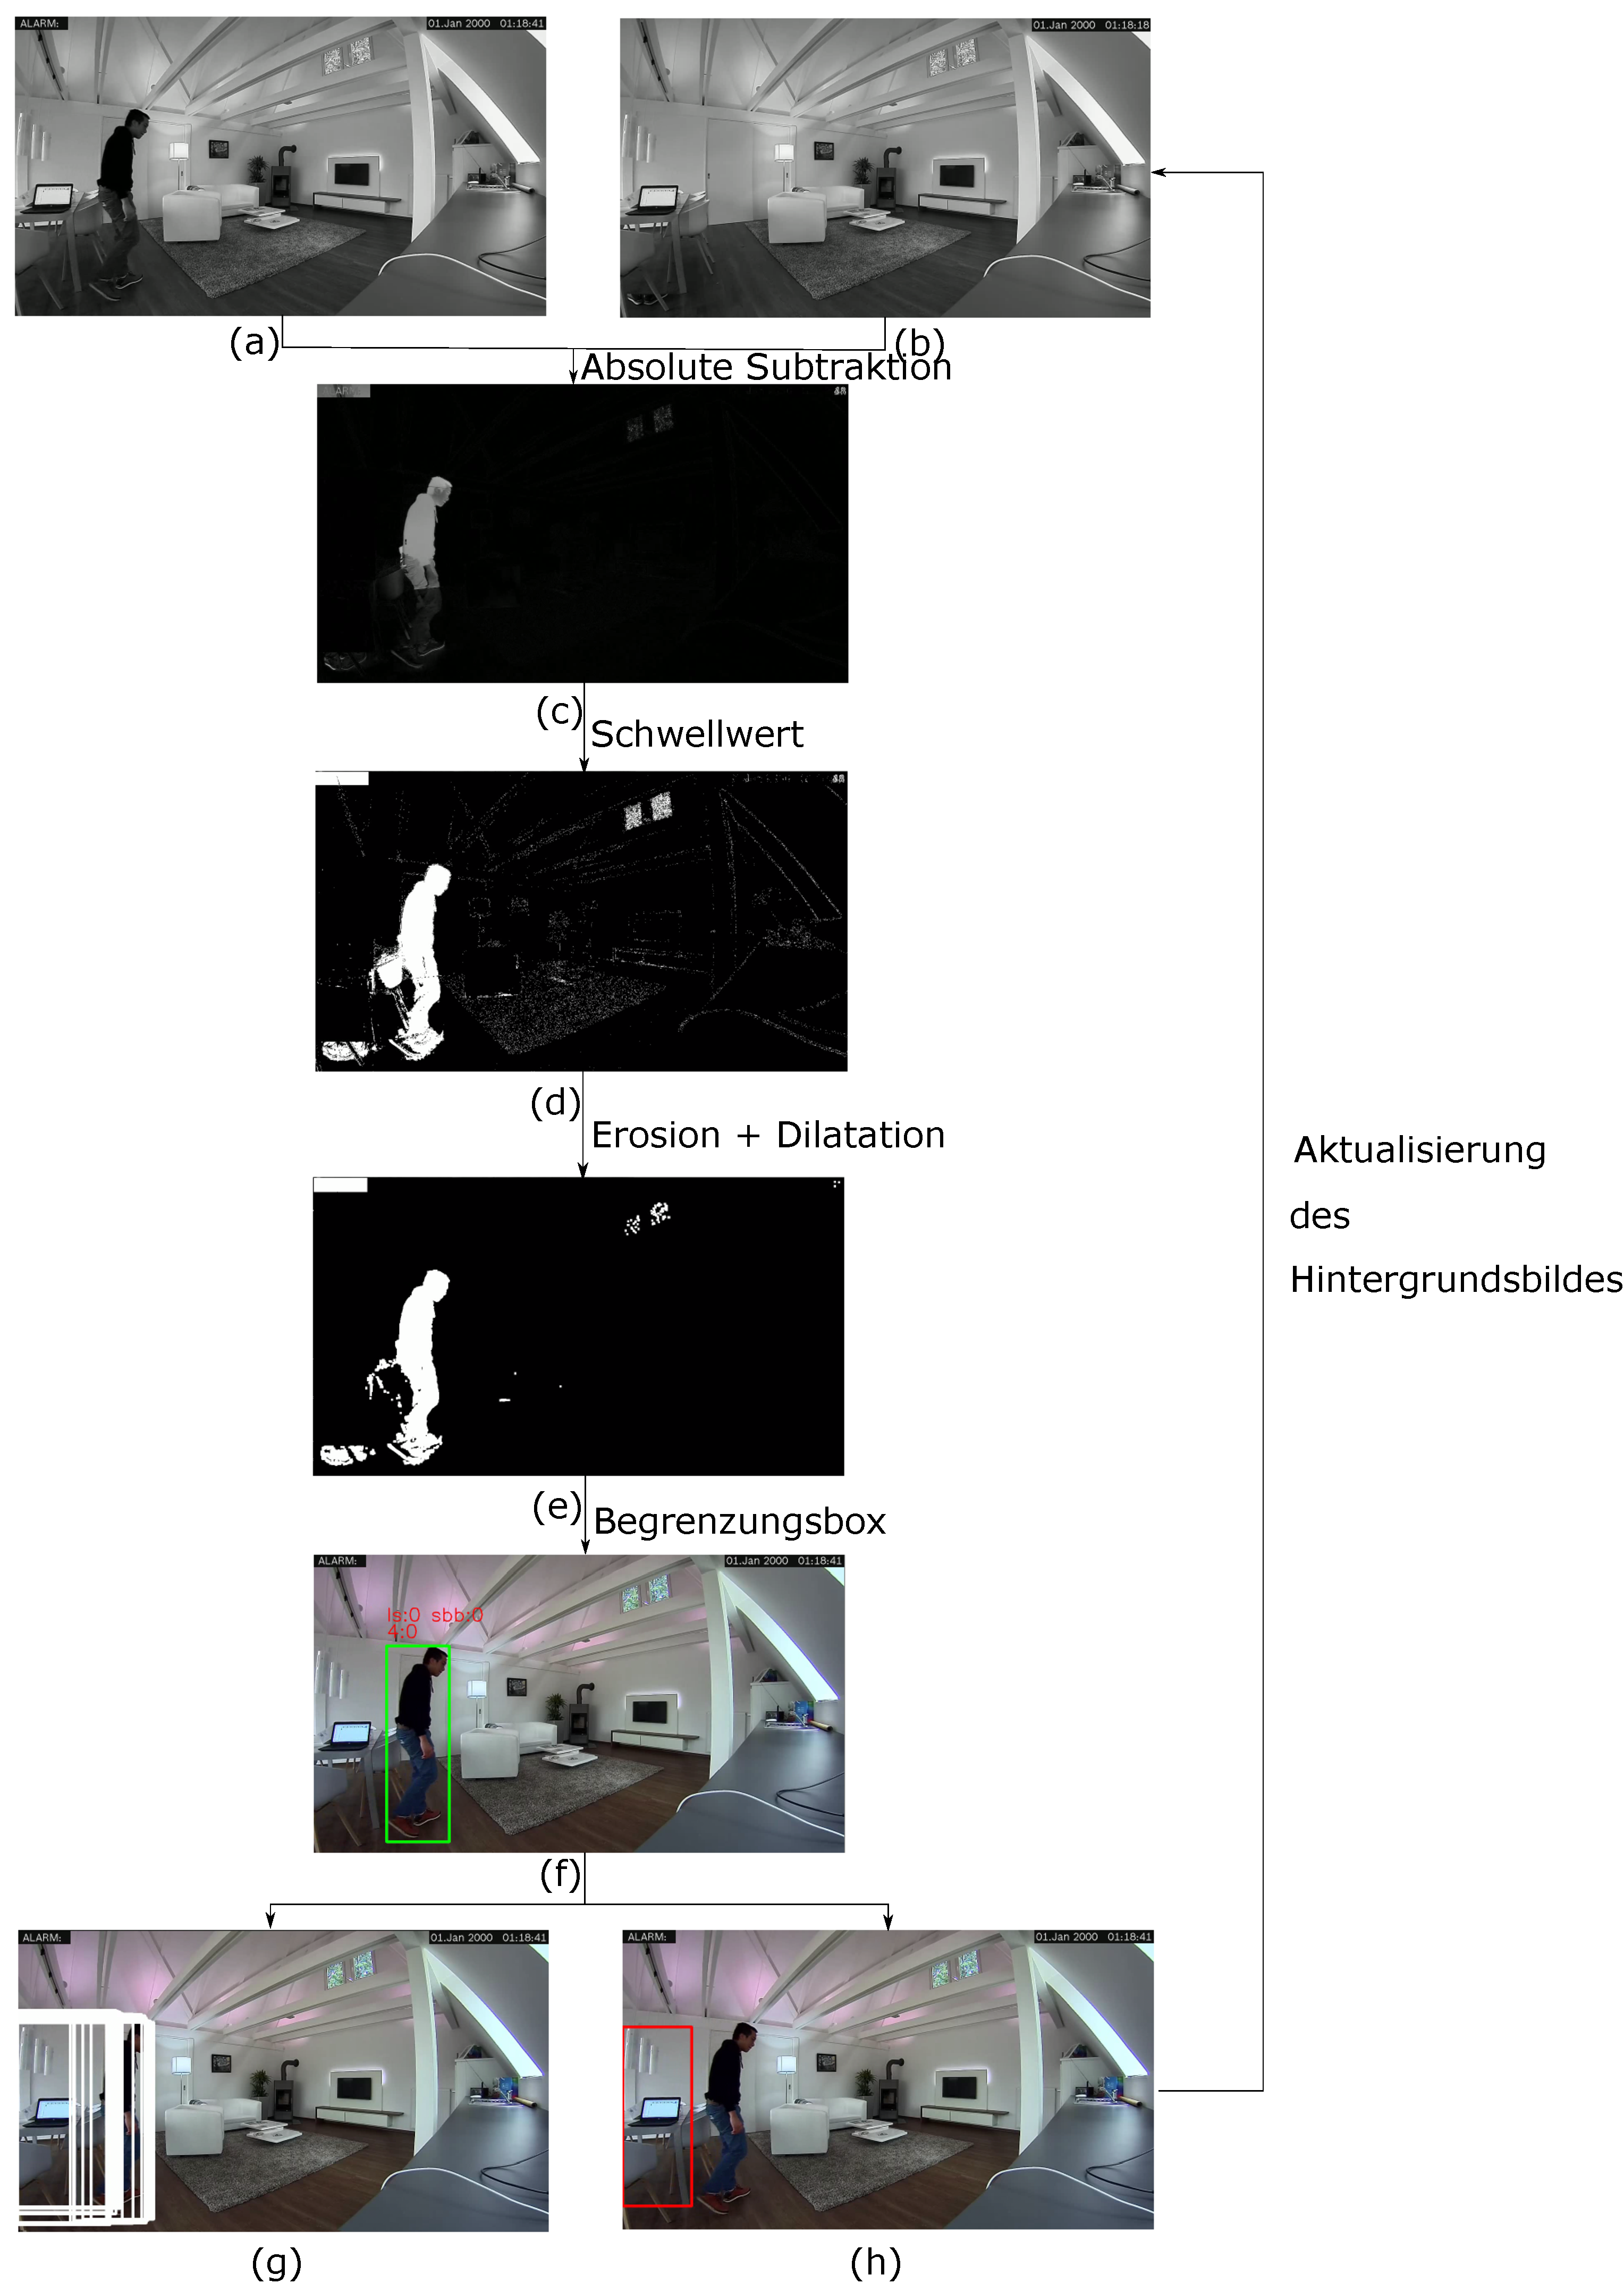
\includegraphics[width=0.9\textwidth]{fig/mymethode4edited.pdf}
	\caption{Video: \glqq{}fallen.mp4\grqq{}. Frame-Nummer: 334. Die Begrenzungsbox $B_i$, die mit einem roten Rechteck markiert ist, �berschneidet sich mit der aktuellen Begrenzungsbox $B_{current}$, die gr�n markiert ist. Das Unterbild in dem roten Rechteck wird auf dem Hintergrundbild aktualisiert.}
	\label{fig:mymethod1}
\end{figure}
\begin{figure}[H]
	\centering
	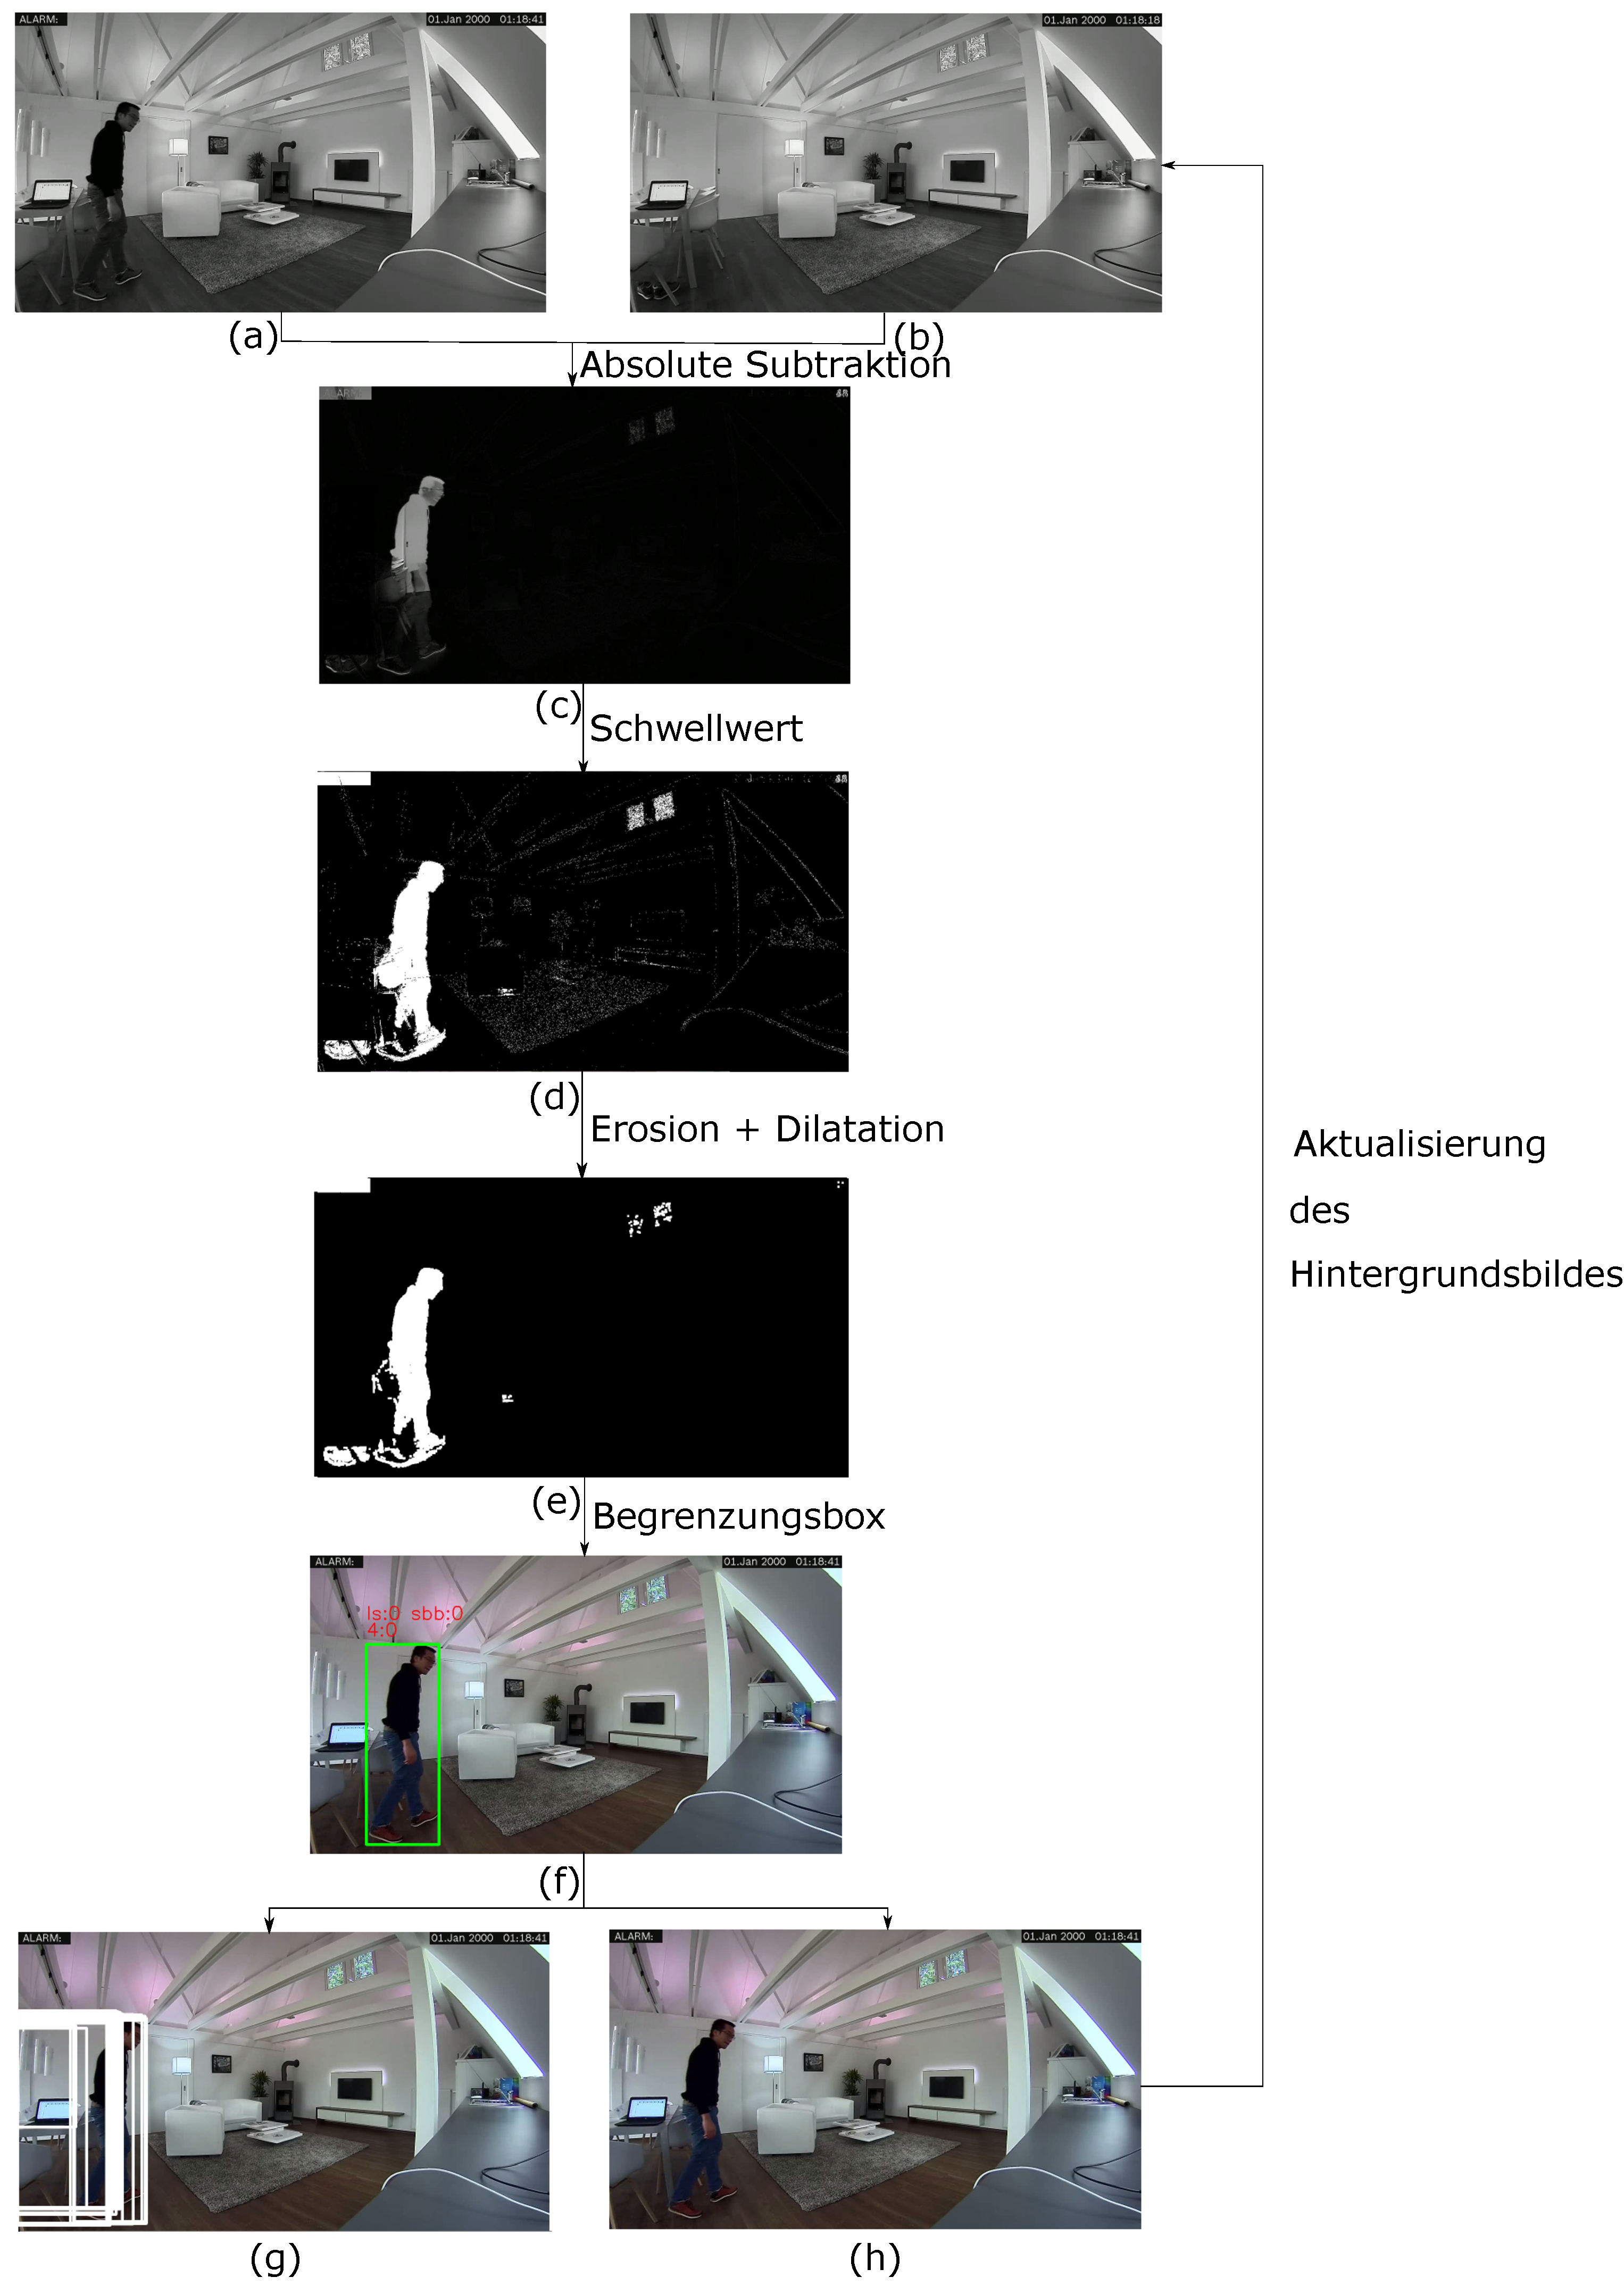
\includegraphics[width=0.9\textwidth]{fig/mymethode3edited.pdf}
	\caption{Video: \glqq{}fallen.mp4\grqq{}. Frame-Nummer: 335. Nach der Aktualisierung des Hintergrundbildes wird die alte Begrenzungsbox $B_i$ gel�scht.}
	\label{fig:mymethod2}
\end{figure}
\begin{figure}[H]			
	\centering
	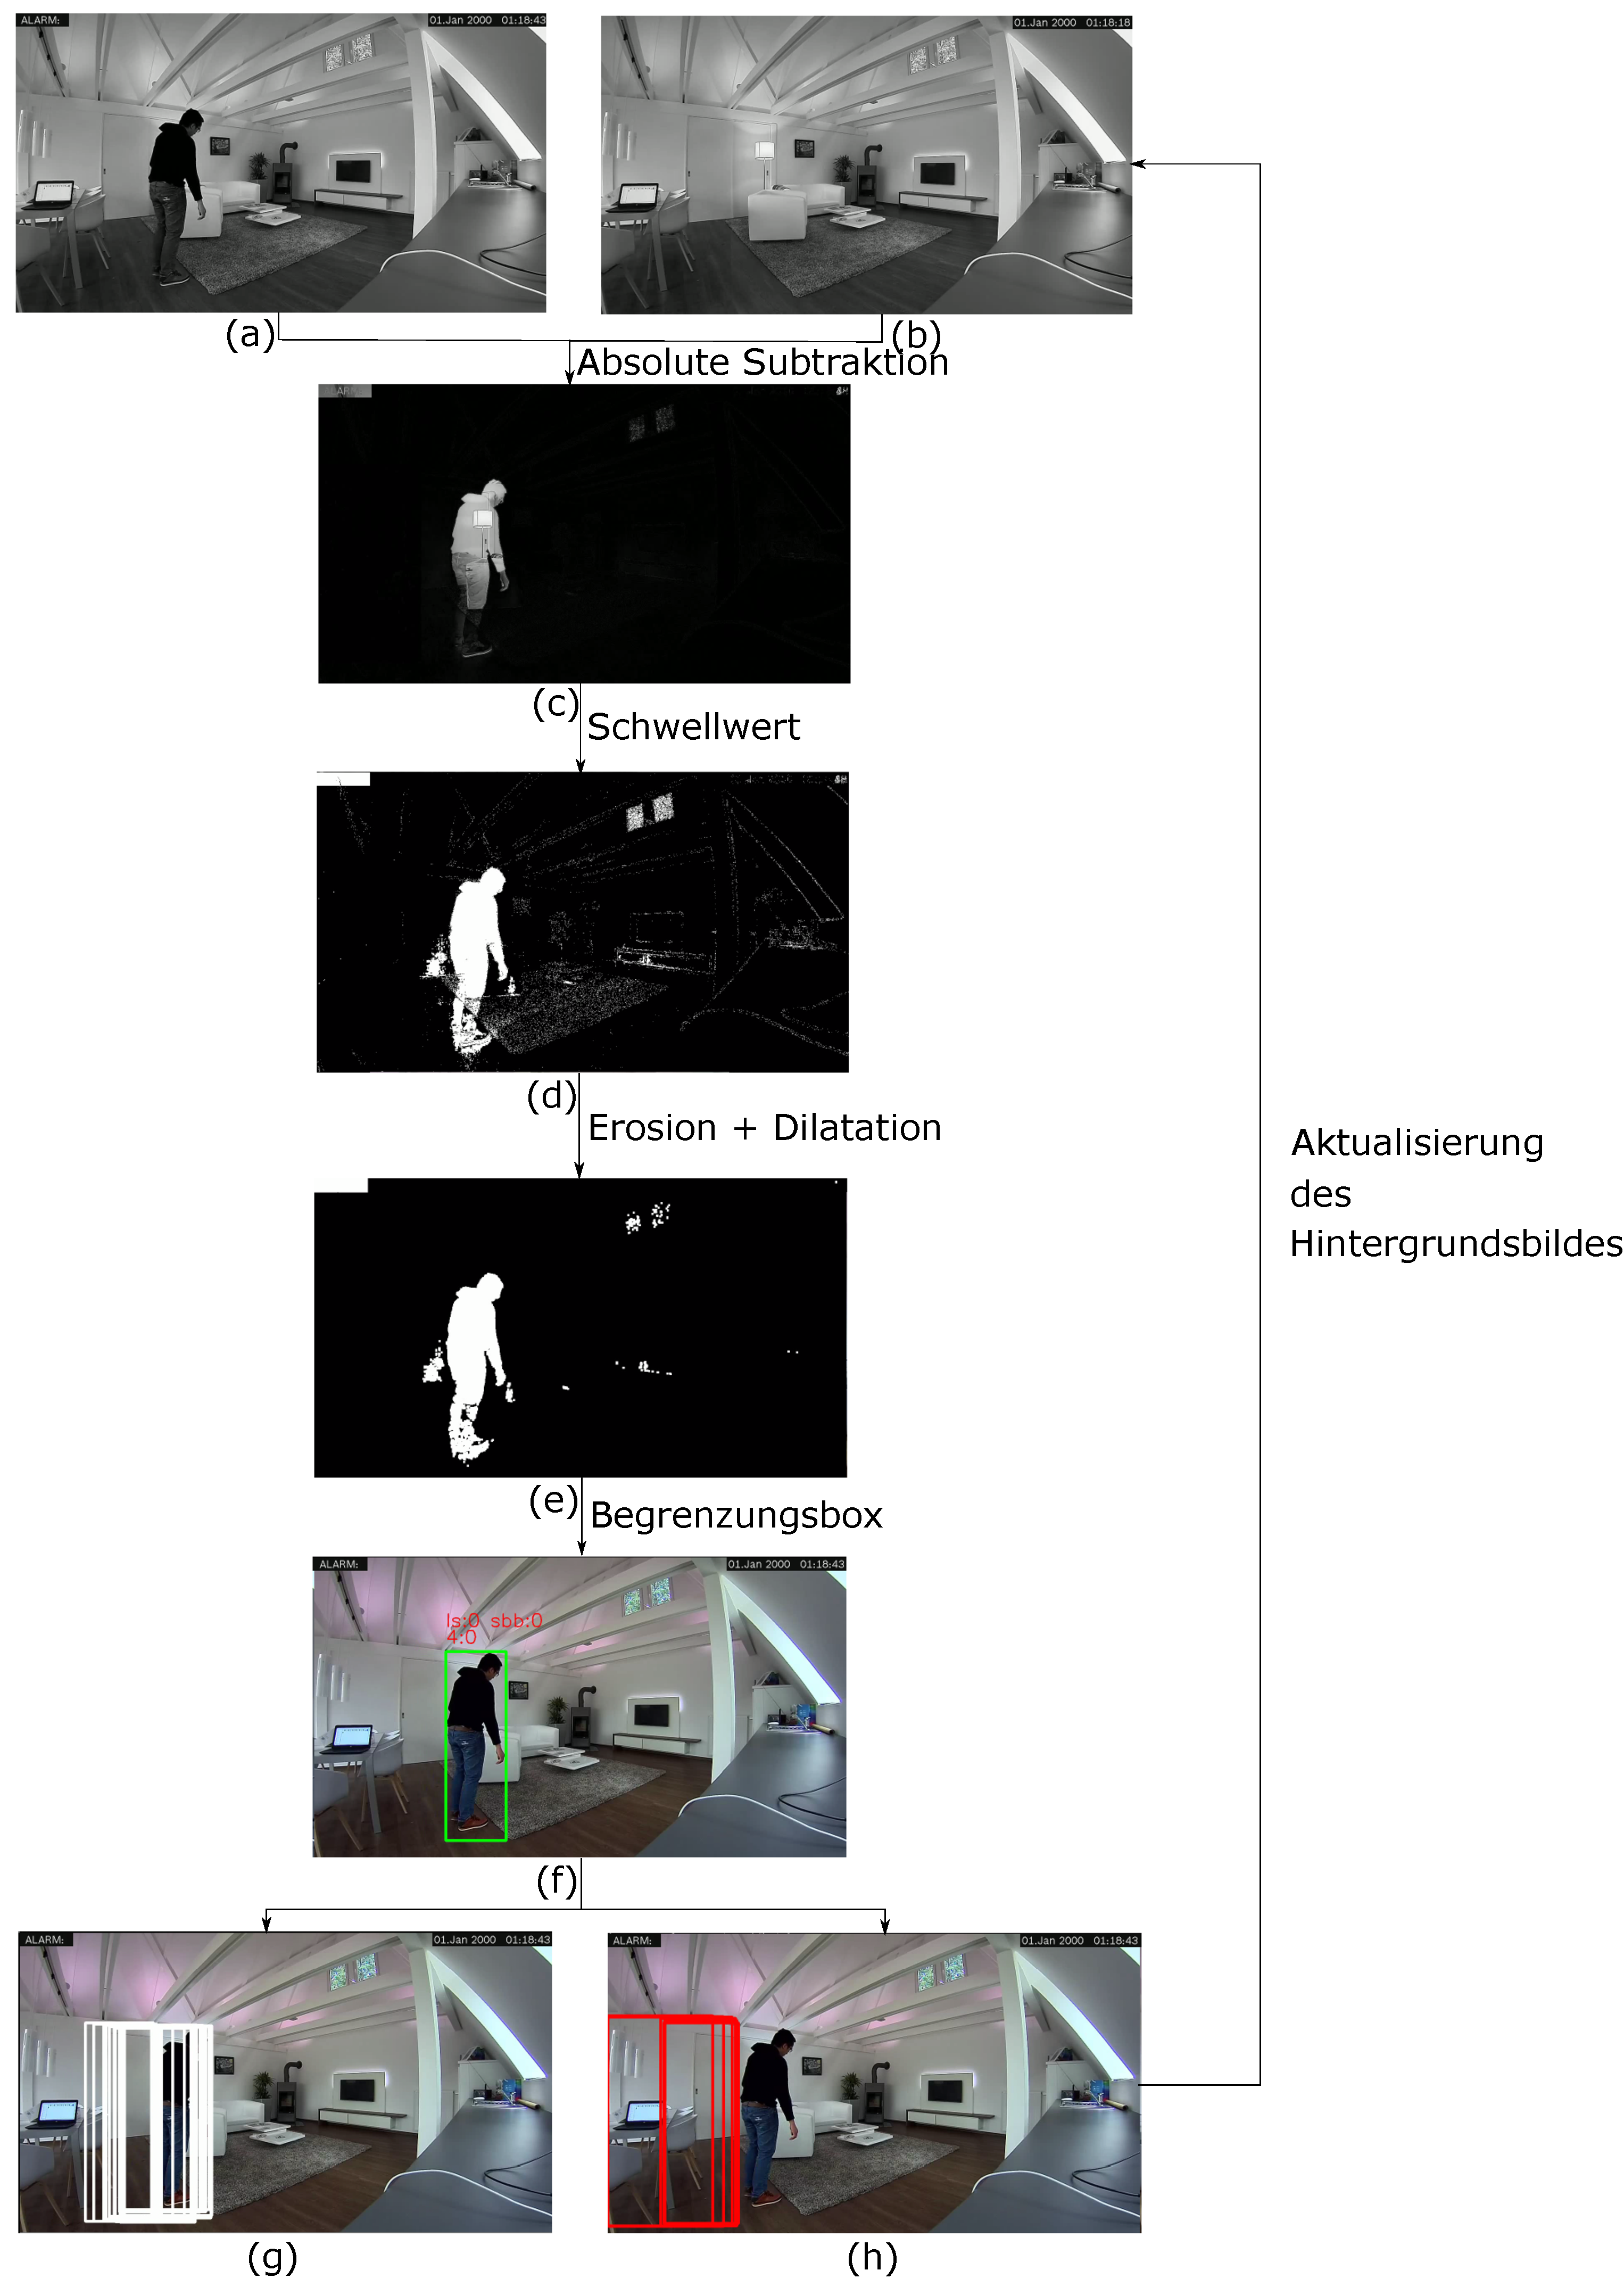
\includegraphics[width=0.9\textwidth]{fig/mymethode2edited.pdf}
	\caption{Video:\glqq{}fallen.mp4\grqq{}. Frame-Nummer: 403. Die Liste der Begrenzungsboxen, die sich nicht mit der aktuellen Begrenzungsbox $B_{current}$ �berschneiden, werden mit den wei�en Rechtecken dargestellt. Die Liste der Begrenzungsboxen, die sich mit der aktuellen Begrenzungsbox $B_{current}$  �berschneiden, werden mit den roten Rechtecken dargestellt. 
	}
	\label{fig:mymethod3}
\end{figure}
Bei der Aktualisierung eines Hintergrundbildes, wo noch kein Hintergrundmodell aufgebaut ist, wird das gesamte Bild als Hintergrund betrachtet. Sonst sollen nur die Pixel, die nicht zum Vordergrund zugeordnet sind, betrachtet werden. Das  wird in ein Grauwertbild mit der Originalgr��e (1280x720) und mit dem Wertbereich $[0,255]$ konvertiert und als ein Hintergrundbild $H$ gespeichert. Der Unterschied zwischen dem aktuellen Grauwertbild $I$ und dem abgespeicherten Hintergrundbild $H$ wird pixelweise mit absoluter Subtraktion gerechnet. Anschlie�end ergibt sich ein Bild $S$, das den Unterschied zwischen dem aktuellen Bild und dem Hintergrundbild  mit den Werten von 0 bis 255 darstellt  (siehe Abbildungen \ref{fig:mymethod1}c, \ref{fig:mymethod2}c, \ref{fig:mymethod3}c). Je geringer der Wert eines Pixels auf dem Bild $S$ ist, desto h�her die Wahrscheinlichkeit, dass der Pixel zum Hintergrund geh�rt. Und umgekehrt je h�her der Wert eines Pixel auf dem Bild $S$ ist, desto h�her ist die Wahrscheinlichkeit, dass das Pixel zum Hintergrund geh�rt. Nach der Berechnung des Unterschiedsbild wird ein Schwellenwert von $50$ angewendet, um ein Bin�rbild zu erzeugen. Alle Pixel mit Werten unter $50$, werden schwarz markiert und alle anderen Wei� (Abbildungen \ref{fig:mymethod1}d, \ref{fig:mymethod2}d, \ref{fig:mymethod3}d).
\\
Der n�chste Schritt ist die Anwendung des �ffnung-Verfahren, um den Rausch der erstellten Silhouette zu entfernen (siehe Abbildungen \ref{fig:mymethod1}e, \ref{fig:mymethod2}e, \ref{fig:mymethod3}e).
Eine Begrenzungsbox (eng. Bounding box) wird an dieser Stelle erstellt, um das sich bewegende Objekt zu begrenzen. Diese Begrenzungsbox wird f�r die Erkennung der K�rperhaltung im n�chsten Abschnitt genutzt.\\
Des weiteren werden die Konturen der Silhouette mithilfe der Methode \inlinecode{C++}{findContours()} von Open-CV  berechnet. Der Aufruf der Methode liefert ein Array von Arrays, wo sich die gruppierten Pixel jeweils zusammen in einem Array befinden. Eine Gruppe von Pixels bildet die Bildpunkte einer der Konturen. F�r die Konturen werden mithilfe der Methode  \inlinecode{C++}{contourArea()} dann Begrenzungsboxen berechnet. Die Person befindet sich in einer der Begrenzungsboxen. Um die Person zu lokalisieren, wird die Begrenzungsbox mit der gr��ten Fl�che ausgew�hlt. Jetzt kann das Hintergrundmodell, mithilfe der Begrenzungsbox $B_{alktuell}$ der Person aktualisiert werden. Abbildungen \ref{fig:mymethod1}f, \ref{fig:mymethod2}f, \ref{fig:mymethod3}f) verdeutlichen diese Schritte. Wenn sich die Person von $P_1$ nach $P_2$ bewegt, wird eine Liste der vergangen Begrenzungsboxen $L_B = \{B_1, B_2, ... , B_n\}$ aktualisiert. Die Liste von Begrenzungsboxen der Person geh�rt zur Historie zu. Bei Aktualisierung des Hintergrundes wird die aktuelle Begrenzungsbox $B_{current}$ mit allen Begrenzungsboxen der Liste $L_B$ verglichen. Wenn eine Begrenzungsbox $B_i$ in $L_B$ mit der aktuellen Begrenzungsbox $B_{current}$ die leer Menge von Schnittpunkten liefert, wird das Unterbild in $B_i$ von dem aktuellem Bild $I$ in das Hintergrundbild $H$ an der gleichen Position ersetzt und in eine Liste $L^*_B$ verschoben. Auf den Abbildungen \ref{fig:mymethod1}h, \ref{fig:mymethod2}h, \ref{fig:mymethod3}h werden die Unterbilder mit Begrenzungsboxen in $L^*_B$, die mit rot markiert sind, in das Hintergrundbild ersetzt. Die Liste $\hat{L}_B = L_B \backslash L^*_B$ enth�lt alle vergangenen Begrenzungsboxen, die keine Schnittpunkte mit der aktuellen Begrenzungsbox $B_{current}$ haben. Die Liste $\hat{L}_B$ wird auf den Abbildungen \ref{fig:mymethod1}g, \ref{fig:mymethod2}g, \ref{fig:mymethod3}g mit wei�er Farbe dargestellt. Au�erdem wird die Begrenzungsbox $B_{current}$ mit gr�ner Farbe auf den Abbildungen \ref{fig:mymethod1}f, \ref{fig:mymethod2}f, \ref{fig:mymethod3}f gezeigt. Nach jeder Aktualisierung des Hintergrundbildes werden alle Elemente der Liste $L^*_B$ gel�scht und die Liste $L_B$ enth�lt nur die Begrenzungsboxen, die mit der aktuellen Begrenzungsbox $B_{alktuell}$ nicht �berschneiden. \\
\subsubsection{Zweite Verbesserung (KNN-Plus-ASB)}
Die ASB Methode hat zwei Vorteile. Der erste Vorteil ist, dass die Methode eine L�sung des Problems ist, wenn eine Person beispielsweise stillsteht. Nach einer bestimmten Zeit wird die Person fehlerhaft in das Hintergrundmodell integriert und so nicht mehr als der Vordergrund erkannt. Der zweite Vorteil ist eine Verbesserung der Verarbeitungszeit, da bei der anderen Methode aus Kapitel \ref{sec:grunglagen_hintergrundsub} eine Liste von Hintergrundbildern gebraucht wird, um das Hintergrundmodell aufzubauen. Aber mit der obengenannten Verbesserung sind nur das Hintergrundbild und das aktuelle Bild n�tig. So wird die ben�tigte Rechenleistung als auch Speicherverbrauch reduziert.\\
Da das Hintergrundmodell nur an Teile des aktuellen Bildes aktualisiert wird, werden kleine �nderungen am Hintergrundbild nicht betrachtet. Daher entsteht viel Rausch im Bin�rbild nach der Hintergrundsubtraktion. Die Aktualisierungen am Hintergundmodell werden nur unter Bedingungen durchgef�hrt. Diese Bedingungen sind dann erf�hlt, wenn sich die Person im Raum bewegt, sonst werden keine Aktualisierungen durchgef�hrt. Im allgemeinen macht die ASB-Methode folgendes: Durch eine Bewegung wird das Hintergrundbild nur an den alten Begrenzungsboxen (wei�en Boxen in Abbildungen \ref{fig:mymethod1} g, \ref{fig:mymethod2} g, \ref{fig:mymethod3}g), die nicht mit aktueller Bewegung �berschneiden, aktualisiert. Die KNN-Plus-ASB-Methode: Ein Bin�rbild wird mit der \acs{KNN} Methode erstellt. Aus dem Bin�rbild wird eine Silhouette mit einer Begrenzungsbox beschr�nkt. Das Hintergrundbild au�er der Bereich der Begrenzungsbox wird aktualisiert.
Die beiden genannten Verbesserungen werden im n�chsten Abschnitt verglichen.
\newpage
\subsection{Ergebnisse der Verbesserungen am Hintergrundsubtraktion-Verfahren}
Um die Qualit�t der Silhouette bewerten zu k�nnen, wird die Silhouette mit dem Ground-Truth verglichen, was eine Silhouette ohne Rausch bildet. Das Ground-Truth-Modell wurde manuell erstellt, um sicherzustellen, dass sich kein Rausch in der Silhouette befindet. Um die Vergleiche durchzuf�hren, werden die Methoden \glqq{}Mean Squared Error\grqq{} und \glqq{}Structural Similarity Measure\grqq{} verwendet. Die erste Vergleich ist die (ASB-Methode). Der zweite Vergleich die KNN-Plus-ASB-Methode. 
Die Formel von \glqq{}Mean Squared Error\grqq{} wird wie folgt beschrieben\cite{kapadia2017mathematical}:\\
\begin{equation}
MSE = \frac{1}{m n } \sum \limits_{i=0}^{m -1} \sum \limits_{j=0}^{n -1} [ I(i, j) - K (i, j)]^2
\end{equation}
wobei $m$ und $n$ die Breite und H�he des Bildes sind und $MSE$ die durchschnittliche Summe der quadratischen Differenz aller Pixel bildet. Je kleiner der $MSE$ Wert ist, desto �hnlicher sind die verglichenen Bilder.  \glqq{}Structural Similarity Measure\grqq{} wird in \cite{wang2004image} vorgestellt. Um strukturelle Ver�nderungen zu erkennen, kommt \glqq{}Structural Similarity Measure\grqq{} zur Qualit�tsbewertung dazu und wird wie folgt berechnet\cite{wang2004image}:
\begin{equation}
SSIM (x, y) = \frac{(2\mu_x \mu_y + c_1)(2\sigma_{xy} + c_2)}{(\mu_x^2 + \mu_y^2 + x_1) ({\sigma_x}^2 + {\sigma_y}^2 + c_2)}
\end{equation}
wobei $x=\{x_i | 1, 2 \dots, N\}$ und $y=\{y_i|1, 2 \dots, N\}$ die Positionen des NxN Fensters in jedem Bild beschreibt. $\mu_x$ und $\mu_y$ sind  die Mittelwerte der Pixelintensit�t in x und y Richtung.  $\sigma_x$ und $\sigma_y$ sind Varianzen,  $\sigma_{xy}$ ist Kovarianz von $x$ und $y$. $C_1$ und $C_2$ sind zwei Konstante.  SSIM ist zwischen 0 und 1 beschr�nkt und je h�her der Wert von SSIM ist, desto �hnlicher sind die zwei Bilder. Tabelle \ref{tbl:comparesihoulette} zeigt uns den Unterschied zwischen dem ASB und KNN-Plus-ASB. Es ist deutlich zu erkennen, dass die zweite Verbesserung bessere Ergebnisse liefert, weil der \glqq{}MSE\grqq{} Wert kleiner und der \glqq{}SSIM\grqq{} Wert gr��er ist.
\begin{table}[H]
	\begin{center}
		\begin{tabular}{ c  c  c  c  }
			\toprule
			Original & Ground Truth & 1. Verbesserung & 2. Verbesserung \\ 
			\bottomrule
			\raisebox{-\totalheight}{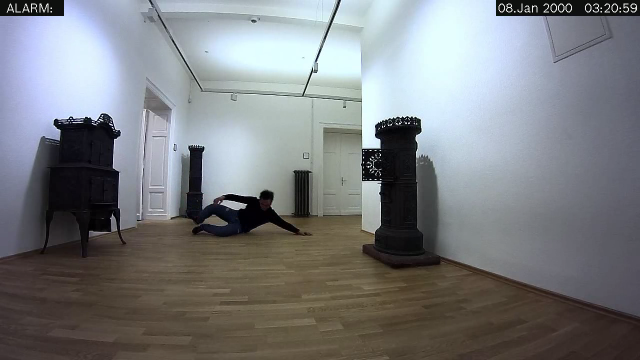
\includegraphics[width=0.25\textwidth]{fig/original1.png}}
			& 
			\raisebox{-\totalheight}{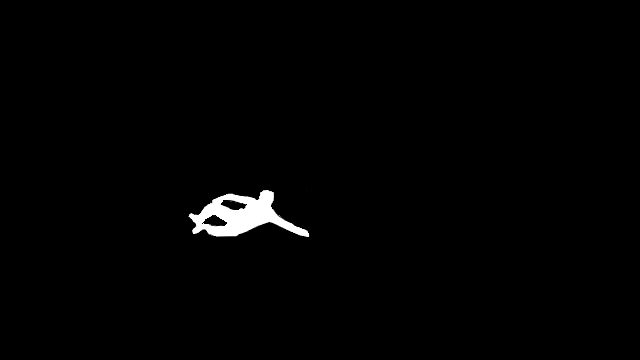
\includegraphics[width=0.25\textwidth]{fig/groundtrue1.png}}
			& 
			\raisebox{-\totalheight}{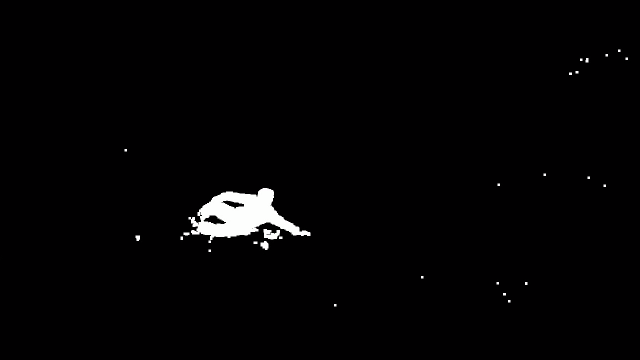
\includegraphics[width=0.25\textwidth]{fig/My1.png}}
			&
			\raisebox{-\totalheight}{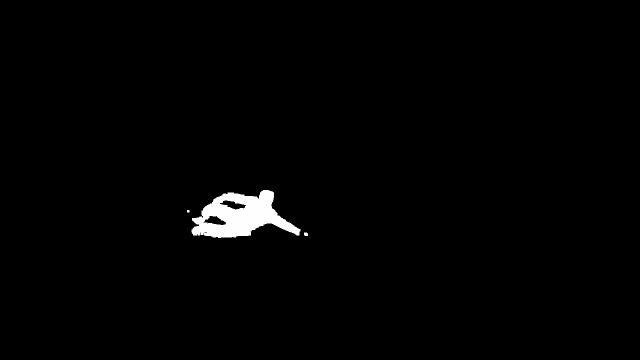
\includegraphics[width=0.25\textwidth]{fig/MOG1.png}}
			\\
			\\
			& & MSE:252,12 SSIM: 0,98 & MSE: 109,36 SSIM: 0,99\\
			 \bottomrule

			\raisebox{-\totalheight}{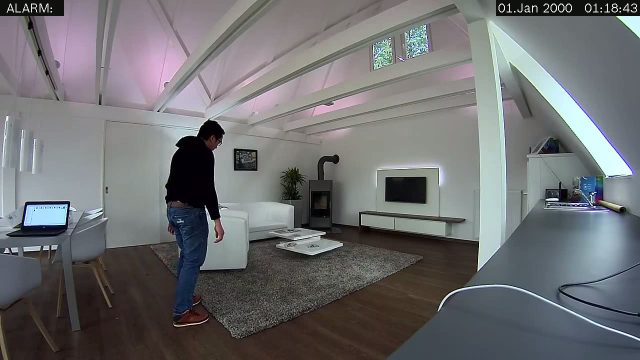
\includegraphics[width=0.25\textwidth]{fig/original2.png}}
			& 
			\raisebox{-\totalheight}{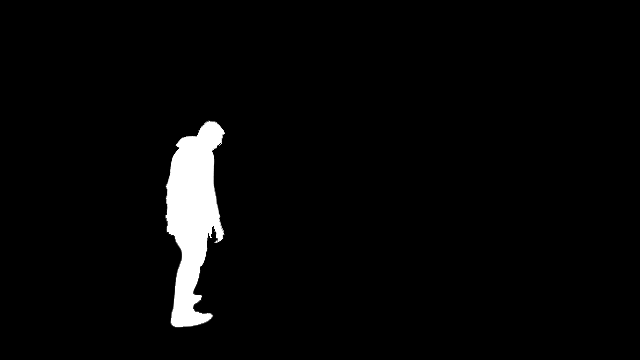
\includegraphics[width=0.25\textwidth]{fig/groundtrue2.png}}
			& 
			\raisebox{-\totalheight}{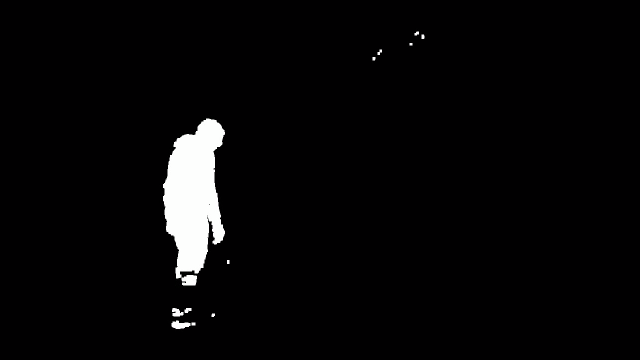
\includegraphics[width=0.25\textwidth]{fig/My2.png}}
			&
			\raisebox{-\totalheight}{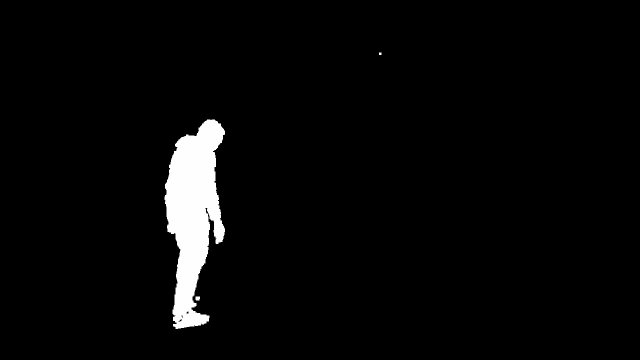
\includegraphics[width=0.25\textwidth]{fig/MOG2.png}}
			\\
			\\
			& & MSE:459,49 SSIM: 0,98 & MSE: 158,21 SSIM: 0,99\\
			\bottomrule
		
			\raisebox{-\totalheight}{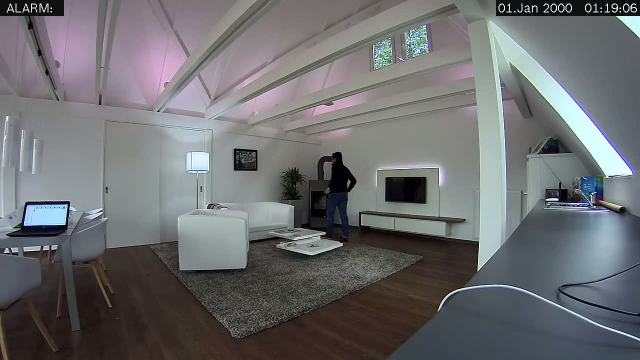
\includegraphics[width=0.25\textwidth]{fig/original3.png}}
			& 
			\raisebox{-\totalheight}{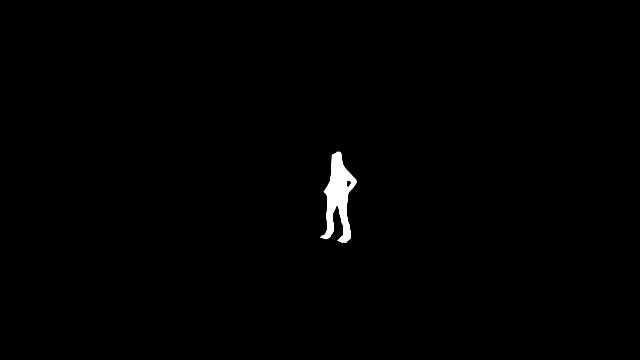
\includegraphics[width=0.25\textwidth]{fig/groundtrue3.png}}
			& 
			\raisebox{-\totalheight}{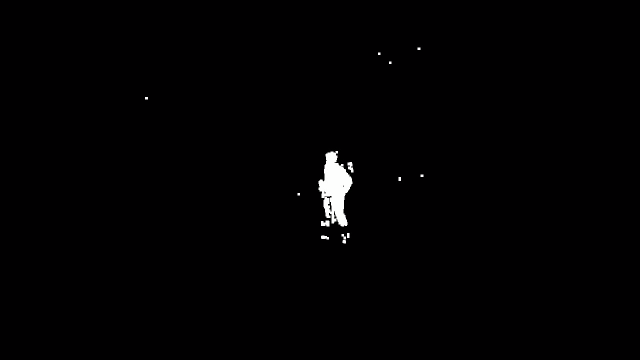
\includegraphics[width=0.25\textwidth]{fig/My3.png}}
			&
			\raisebox{-\totalheight}{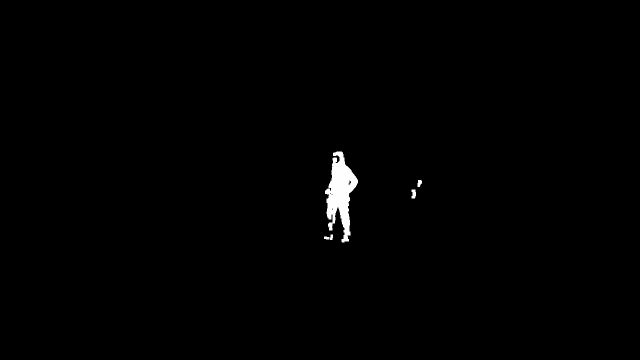
\includegraphics[width=0.25\textwidth]{fig/MOG3.png}}
			\\
			\\
			& & MSE:268,24 SSIM: 0,99 & MSE: 121,59 SSIM: 0,99\\
			\bottomrule
			
			
			\raisebox{-\totalheight}{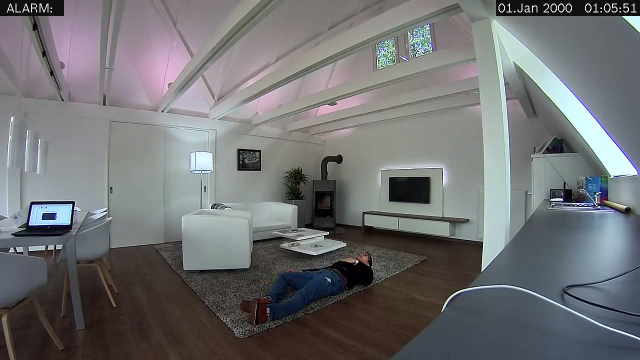
\includegraphics[width=0.25\textwidth]{fig/original4.png}}
			& 
			\raisebox{-\totalheight}{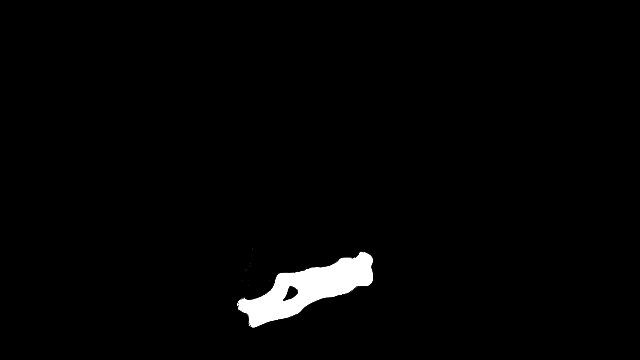
\includegraphics[width=0.25\textwidth]{fig/groundtrue4.png}}
			& 
			\raisebox{-\totalheight}{
\includegraphics[width=0.25\textwidth]{fig/My4.png}}
			&
			\raisebox{-\totalheight}{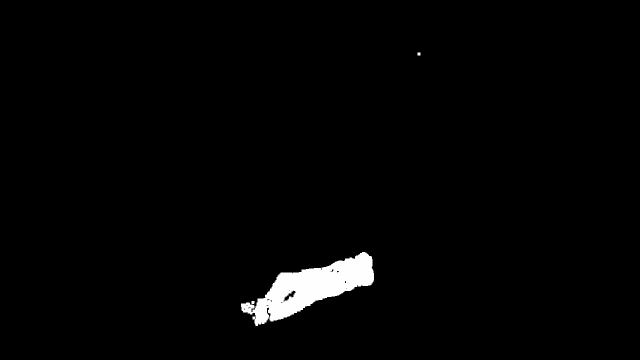
\includegraphics[width=0.25\textwidth]{fig/MOG4.png}}
			\\
			\\
			& & MSE:479,95 SSIM: 0,97 & MSE: 111,75 SSIM: 0,99\\
			\bottomrule
			
			\raisebox{-\totalheight}{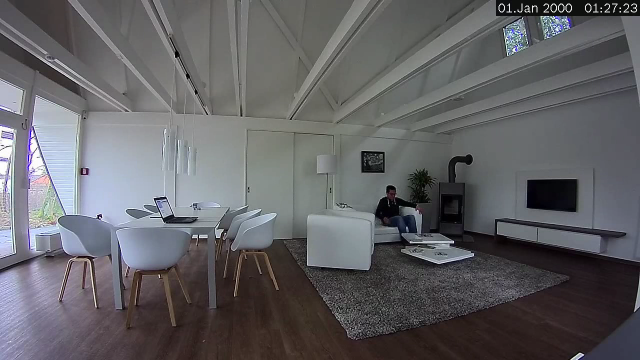
\includegraphics[width=0.25\textwidth]{fig/original5.png}}
			& 
			\raisebox{-\totalheight}{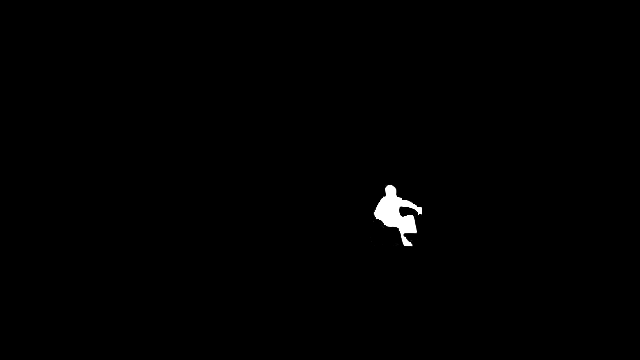
\includegraphics[width=0.25\textwidth]{fig/groundtrue5.png}}
			& 
			\raisebox{-\totalheight}{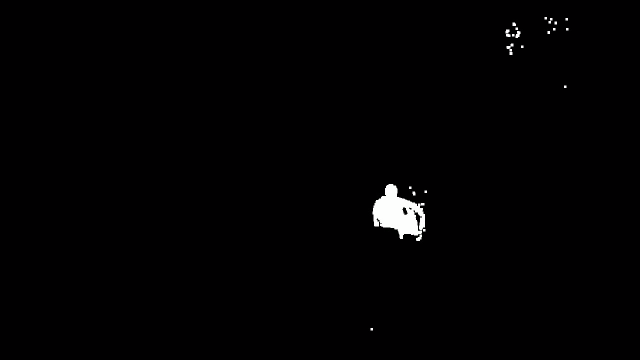
\includegraphics[width=0.25\textwidth]{fig/My5.png}}
			&
			\raisebox{-\totalheight}{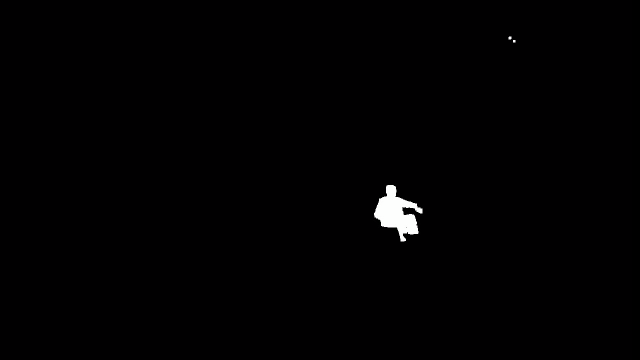
\includegraphics[width=0.25\textwidth]{fig/MOG5.png}}
			\\
			\\
			& & MSE:182,61 SSIM: 0,99 & MSE: 54,42 SSIM: 1.0\\
			\bottomrule
		\end{tabular}
		\caption{Vergleiche von ASB und KNN-Plus-ASB. Je kleiner der \glqq{}MSE\grqq{} Wert ist, desto besser ist das Ergebnis. Je gr��er der \glqq{}SSIM\grqq{} Wert ist, desto besser ist das Ergebnis.}
		\label{tbl:comparesihoulette}
	\end{center}
\end{table}
Diese KNN-Plus-ASB verbessert die Qualit�t der Silhouette und erh�ht auch die Genauigkeit der Sch�tzung der K�rperhaltung, die in n�chstem Abschnitt besprochen wird.  Allerdings, ist die Kombination von \acs{KNN} und \acs{ASB} hat einen Nachteil, dass die Laufzeit sich etwas erh�rt, im Vergleich mit der erster Methode.
Zuletzt kommt noch eine kurz Laufzeitanalyse, um sicherzustellen, dass die Verbesserungen einsetzbar sind und nicht zu hohe Rechenzeit ben�tigen. Aus der Abbildung xyz ist zu entnehmen, dass die Verbesserung ABS eine Laufzeit von xx ms aufweist, wobei KNN-Plus-ASB yy ms ben�tigt.
\section{Sch�tzung der K�rperhaltung mittels Histogrammanalyse}\label{chp:schatzung}
Im Abschnitt \ref{chp:BackgroundSubtraction} wurde eine Silhouette von einer Person durch Hintergrundsubtraktion erstellt. In diesem Abschnitt wird der zweite Meilenstein dieser Arbeit beschrieben. Es geht um die Sch�tzung der K�rperhaltung mit Hilfe von Histogrammanalyse. Wie schon im Kapitel \ref{chp:Grundlageb} beschrieben, basiert die Sch�tzung der K�rperhaltung auf die Forschung von Haritaoglu, Hatwood und Davis in \cite{haritaoglu1998ghost}. Die Histogrammanalyse zur Sch�tzung der K�rperhaltung in dem sogenannten \glqq{}Ghost\grqq{}-System in \cite{haritaoglu1998ghost} wird hier angewendet. Nach der Hintergrundsubtraktion wird ein Bin�rbild erzeugt, welches eine Bewegung in der Szene darstellt. Die Bewegung wird durch eine Begrenzungsbox eingeschr�nkt (siehe Abbildungen \ref{fig:mymethod1}f, \ref{fig:mymethod2}f, \ref{fig:mymethod3}f). Mit Hilfe von dieser Begrenzungsboxen werden die Silhouetten aus dem Bild extrahiert und es wird ein Unterbild erstellt, das nur die Silhouette enth�lt.
Um bei der Histogrammanalyse vergleichbare Ergebnisse f�r unterschiedlich gro�e Silhouetten zu bekommen, muss eine Skalierung vorgenommen werden. Nach der Erzeugung von dem Unterbild wird das Ergebnis zuerst auf 128 Pixel skaliert. Dabei wird das Verh�ltnis von H�he und Breite nicht ver�ndert. Falls das skalierte Bild auf einer Achse kleiner als 128 Pixel geworden ist, dann wird der Rest der verbliebenen Pixel mit Nullen aufgef�llt, wobei das skalierte Bild in der Mitte bleibt (siehe Abbildung \ref{fig:histogramverschiebung}). Das Unterbild wird also immer auf beiden Achsen zentriert mit dem Referenz-Histogramm verglichen.\\
\begin{figure}[H]
	\centering	
	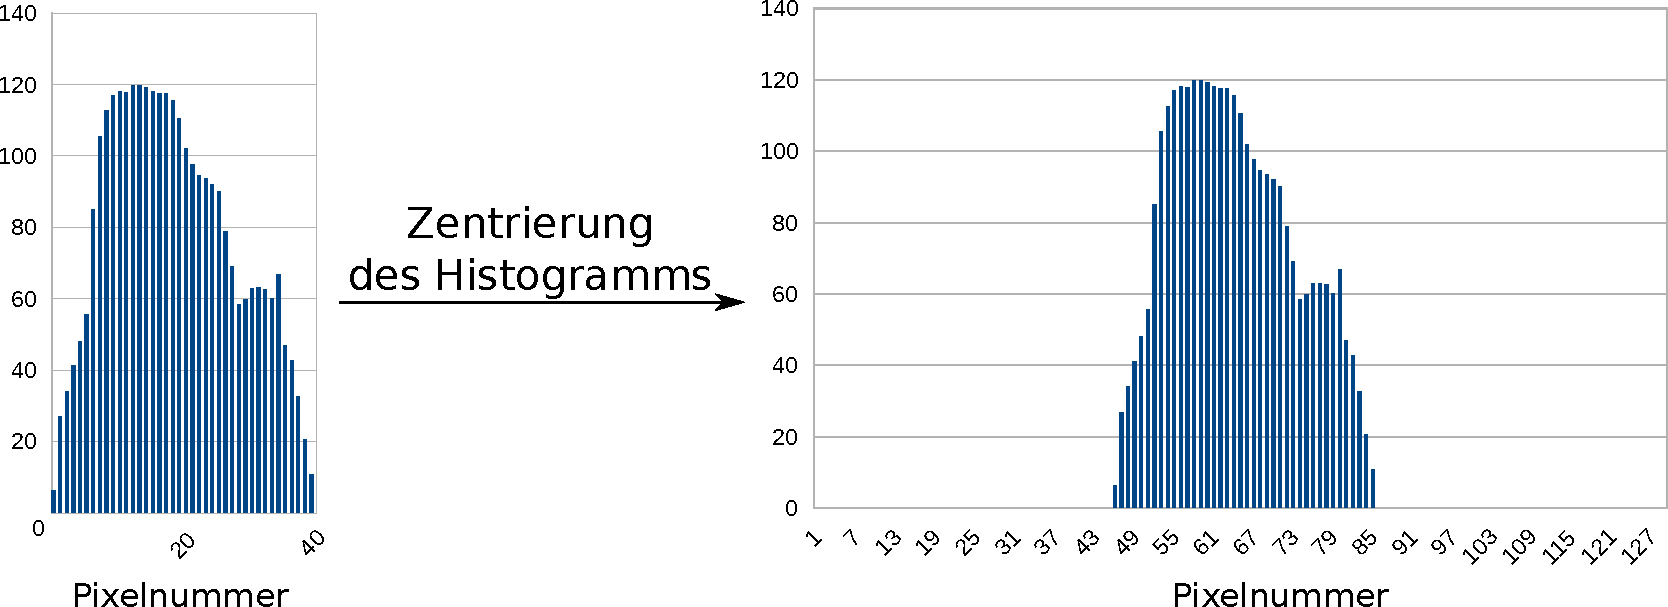
\includegraphics[width=1\textwidth]{fig/histogramverschiebung.pdf}
	\caption{Wenn die L�nge eines Histogramms kleiner als 128 Pixel ist, wird das Histogramm auf einem 128 Pixel lang Histogramm abgebildet. Die Werte des originalen Histogramms werden in der Mitte des neuen Histogramm zentriert.}
	\label{fig:histogramverschiebung}
\end{figure}

Wie schon im Abschnitt \ref{sec:Histogrammanalyse} beschrieben, k�nnen mit der Formel \ref{eq:loglikelyhood} die berechneten Histogramme mit den vordefinierten normalisierten Referenz-Histogrammen (siehe Abbildung \ref{fig:histogramm}) verglichen werden. Je gr��er das Ergebnis aus der Formel \ref{eq:loglikelyhood} ist, desto h�her ist die Wahrscheinlichkeit, dass die Person die betrachtete K�rperhaltung annimmt. Die Abbildung \ref{fig:schatzung} zeigt, wie sich aus dem zweiten Meilenstein die Sch�tzung der K�rperhaltung zu Stande kommt. Die Abbildungen \ref{fig:schatzung1}, \ref{fig:schatzung2} und \ref{fig:schatzung3} repr�sentieren die Sch�tzung der K�rperhaltung in graphische Beispiele, um den zweiten Schritt klarzustellen.
\begin{figure}[H]
	\centering	
	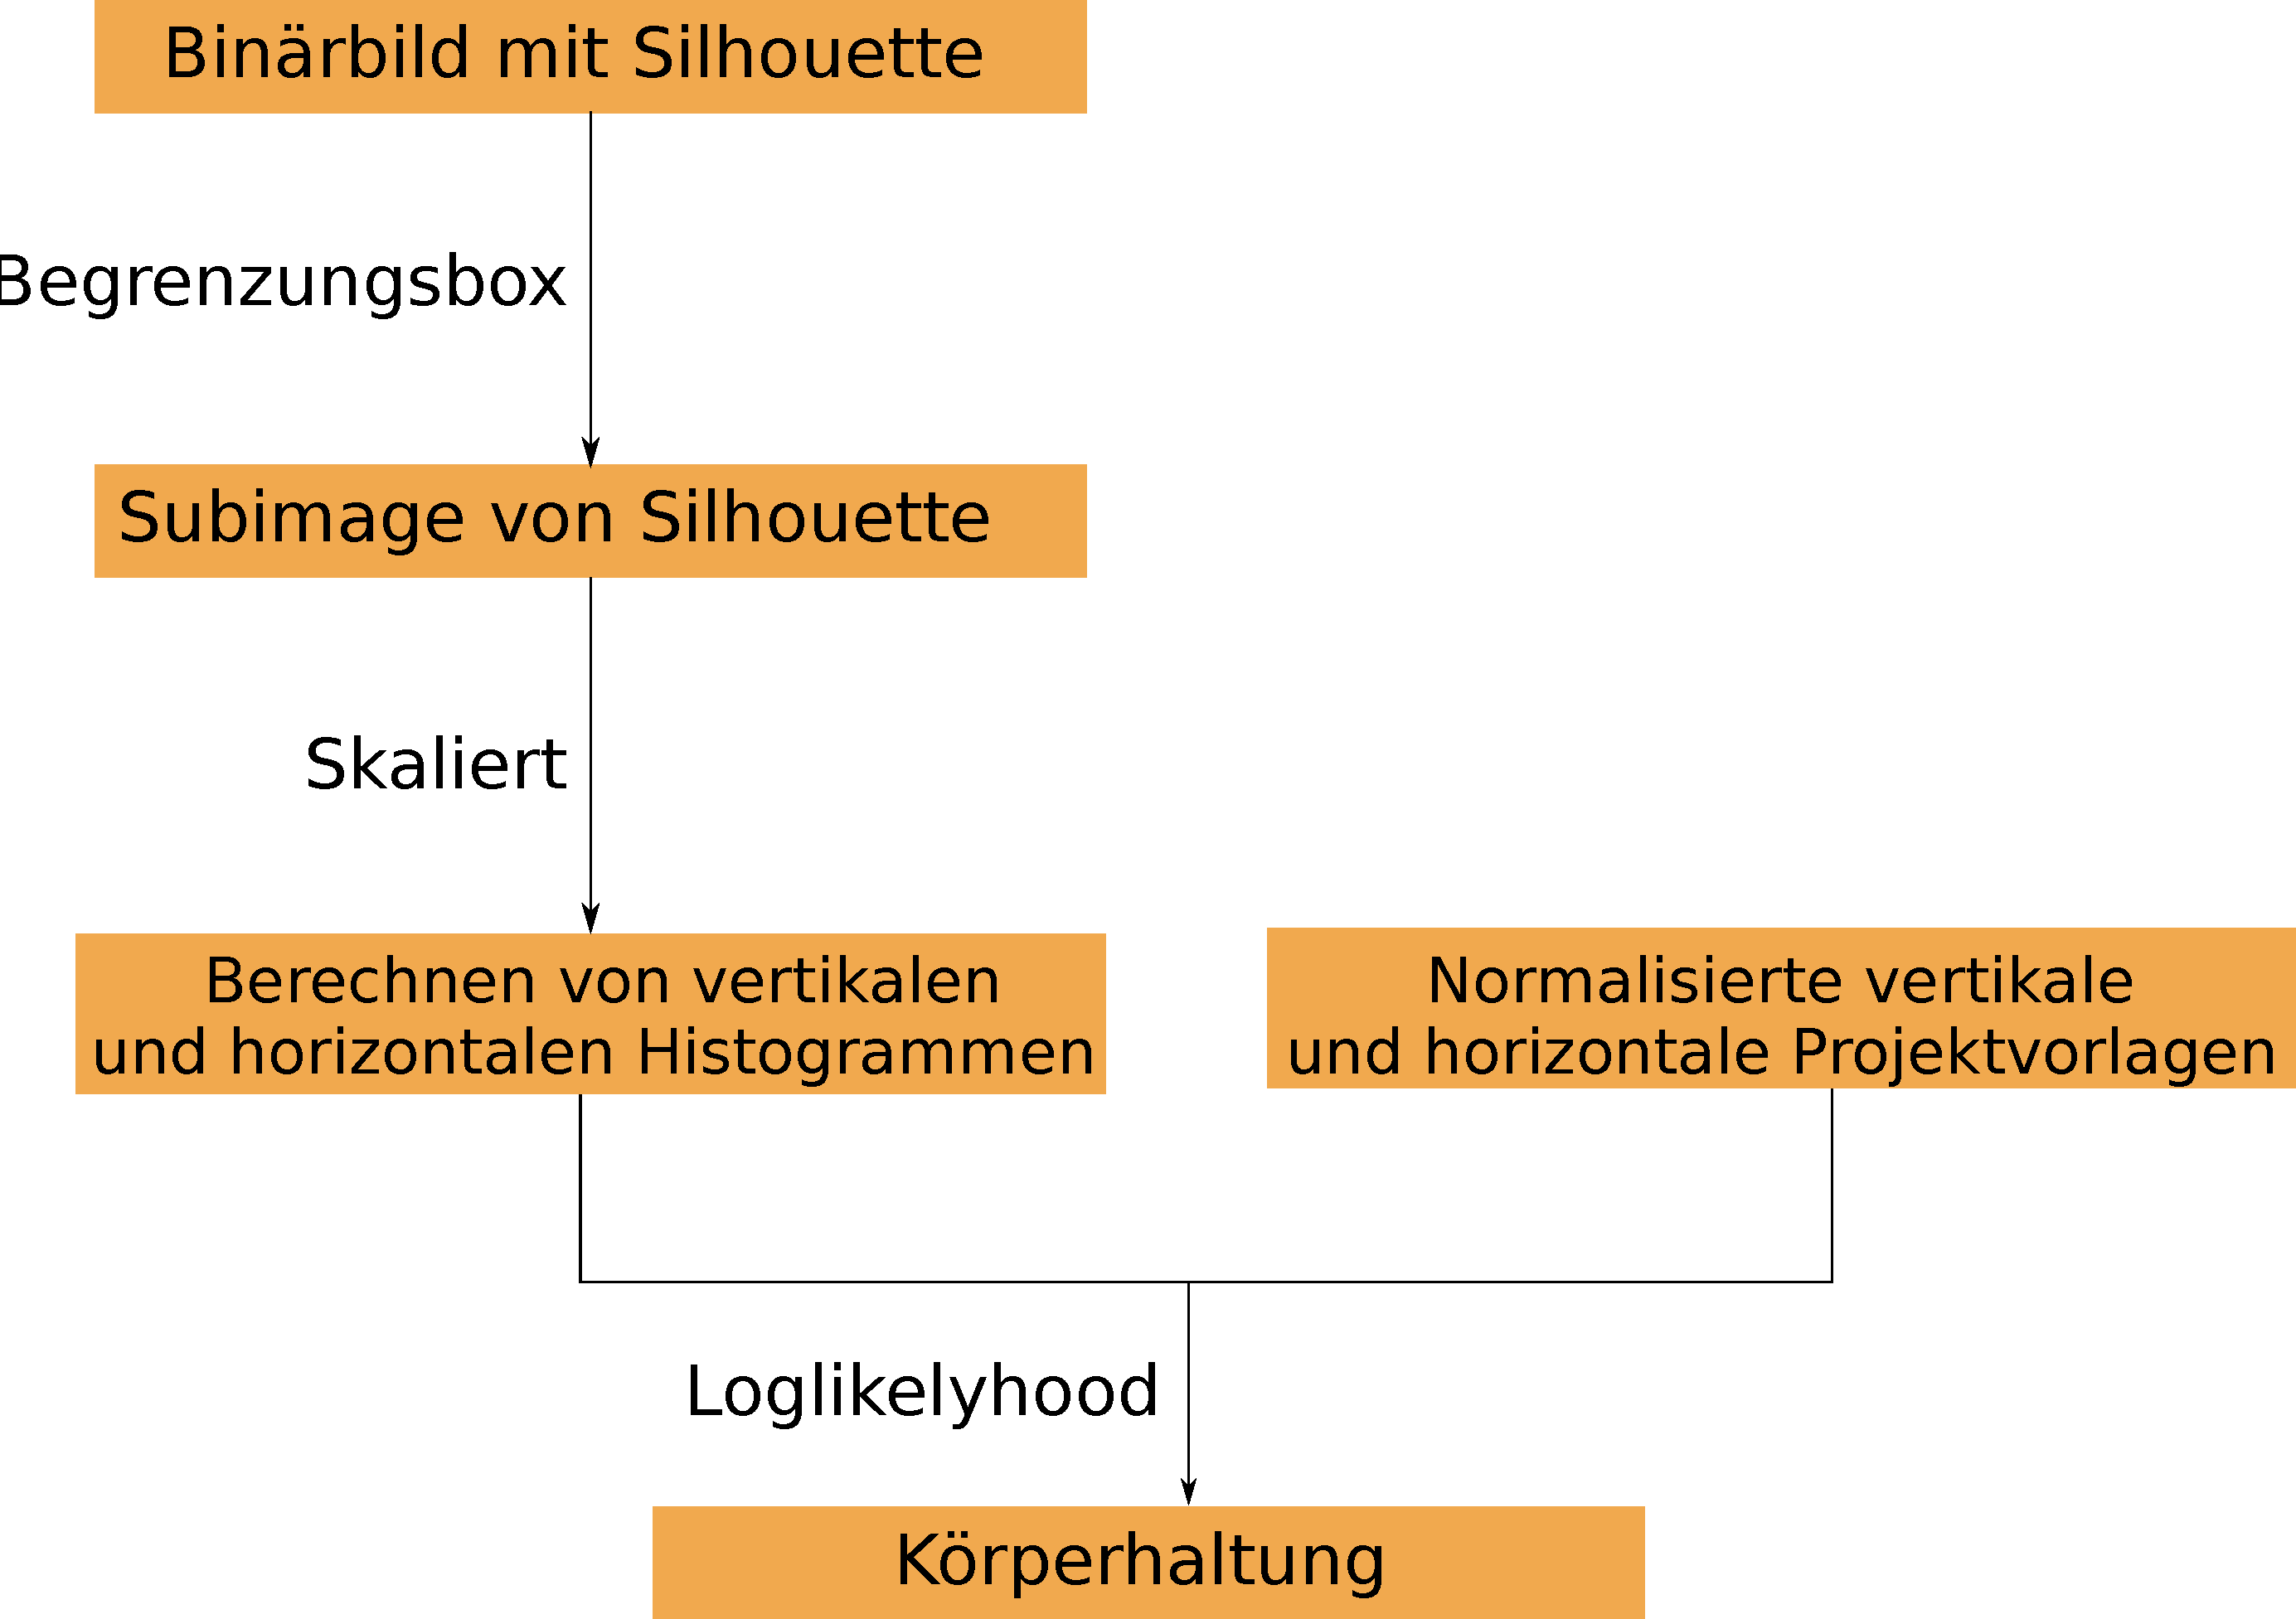
\includegraphics[width=0.95\textwidth]{fig/schatzung.pdf}
	\caption{Der zweite Meilenstein ist die Sch�tzung der K�rperhaltung. Das Ausgabebin�rbild des ersten Meilensteins wird mit einer Begrenzungsbox beschr�nkt, um ein Unterbild von der Silhouette zu erstellen. Das Unterbild wird dann skaliert und die vertikalen und horizontalen Histogramme des skalierten Unterbildes werden berechnet. Diese Histogramme werden mit den Referenz-Histogrammen verglichen, um die K�rperhaltung auf dem Unterbild zu bestimmen.}
	\label{fig:schatzung}
\end{figure}

\begin{figure}[H]
	\centering
	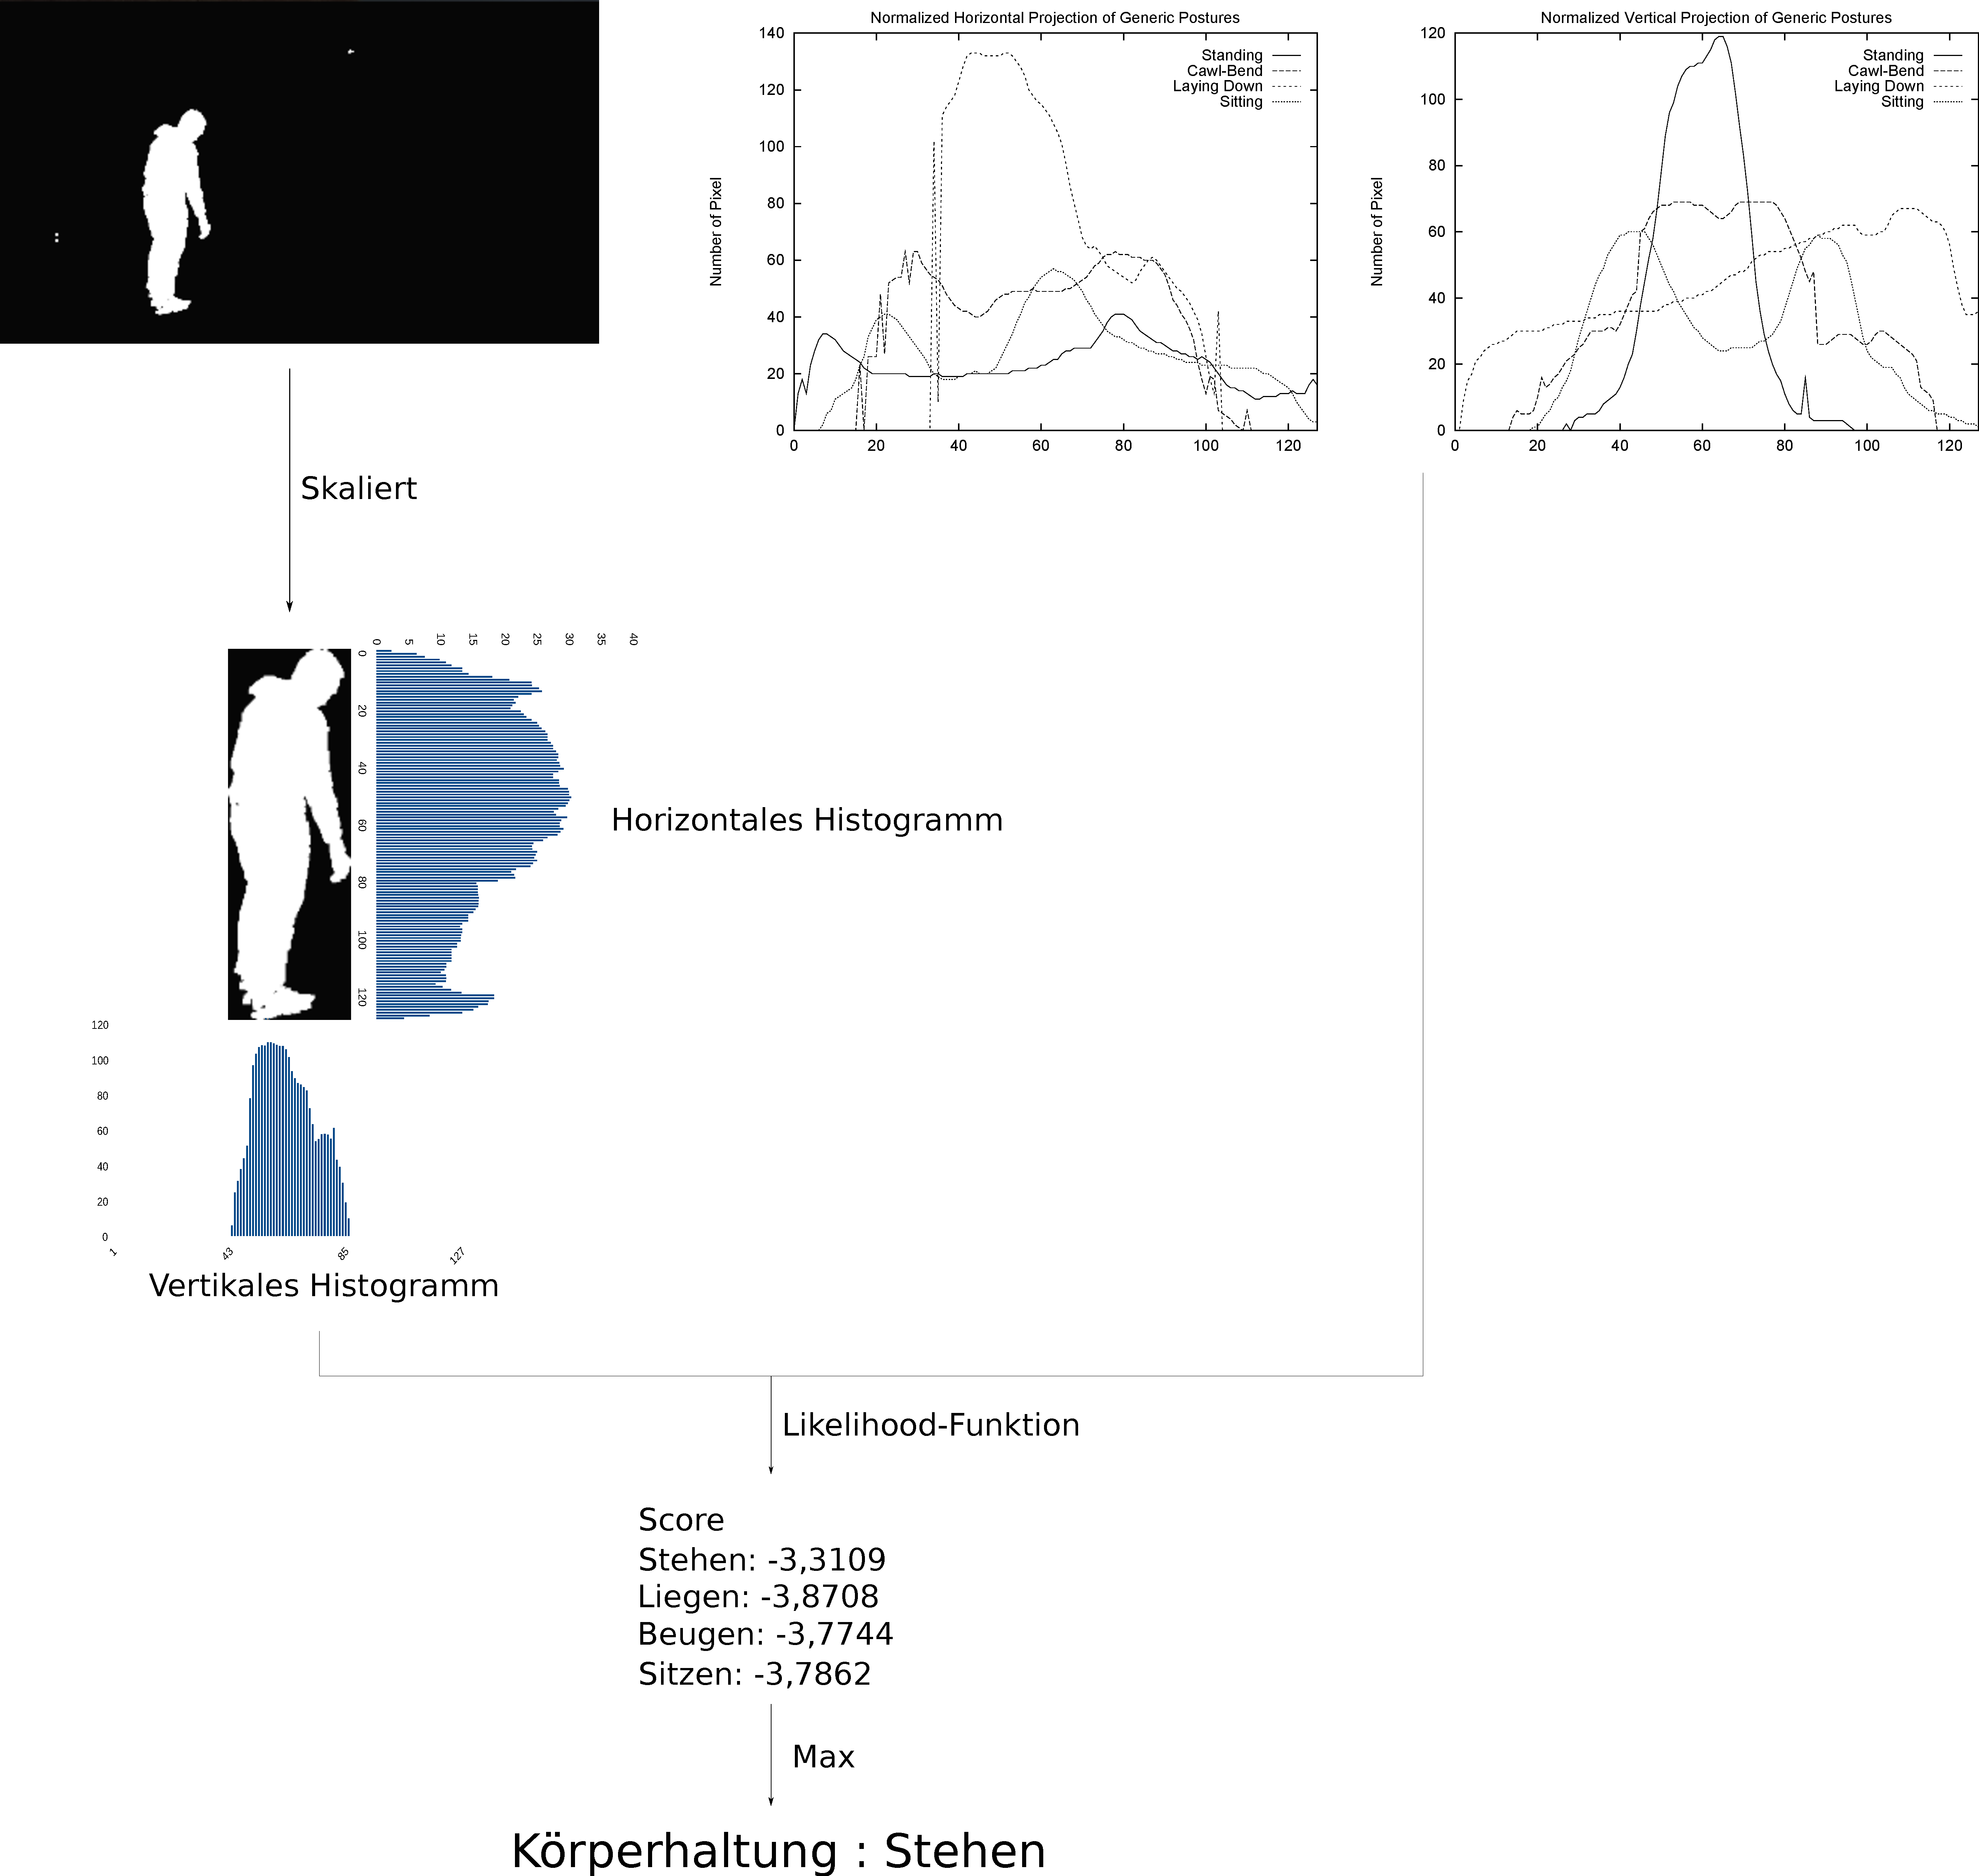
\includegraphics[width=1\textwidth]{fig/schatzung1.pdf}
	\caption{Ein Beispiel f�r einen Prozess von Sch�tzung einer Silhouette beim Stehen. Die Silhouette des Bin�rbildes wird zuerst durch eine Begrenzungsbox extrahiert. Die vertikalen und horizontalen Histogramme der Silhouette werden dann berechnet und mit den entsprechenden Referenz-Histogrammen jeder generischen K�rperhaltung verglichen. Die K�rperhaltung, die nach dem Vergleich den gr��ten Wert hat, wird f�r die Silhouette genommen.}
	\label{fig:schatzung1}
\end{figure}

\begin{figure}[H]
	\centering
	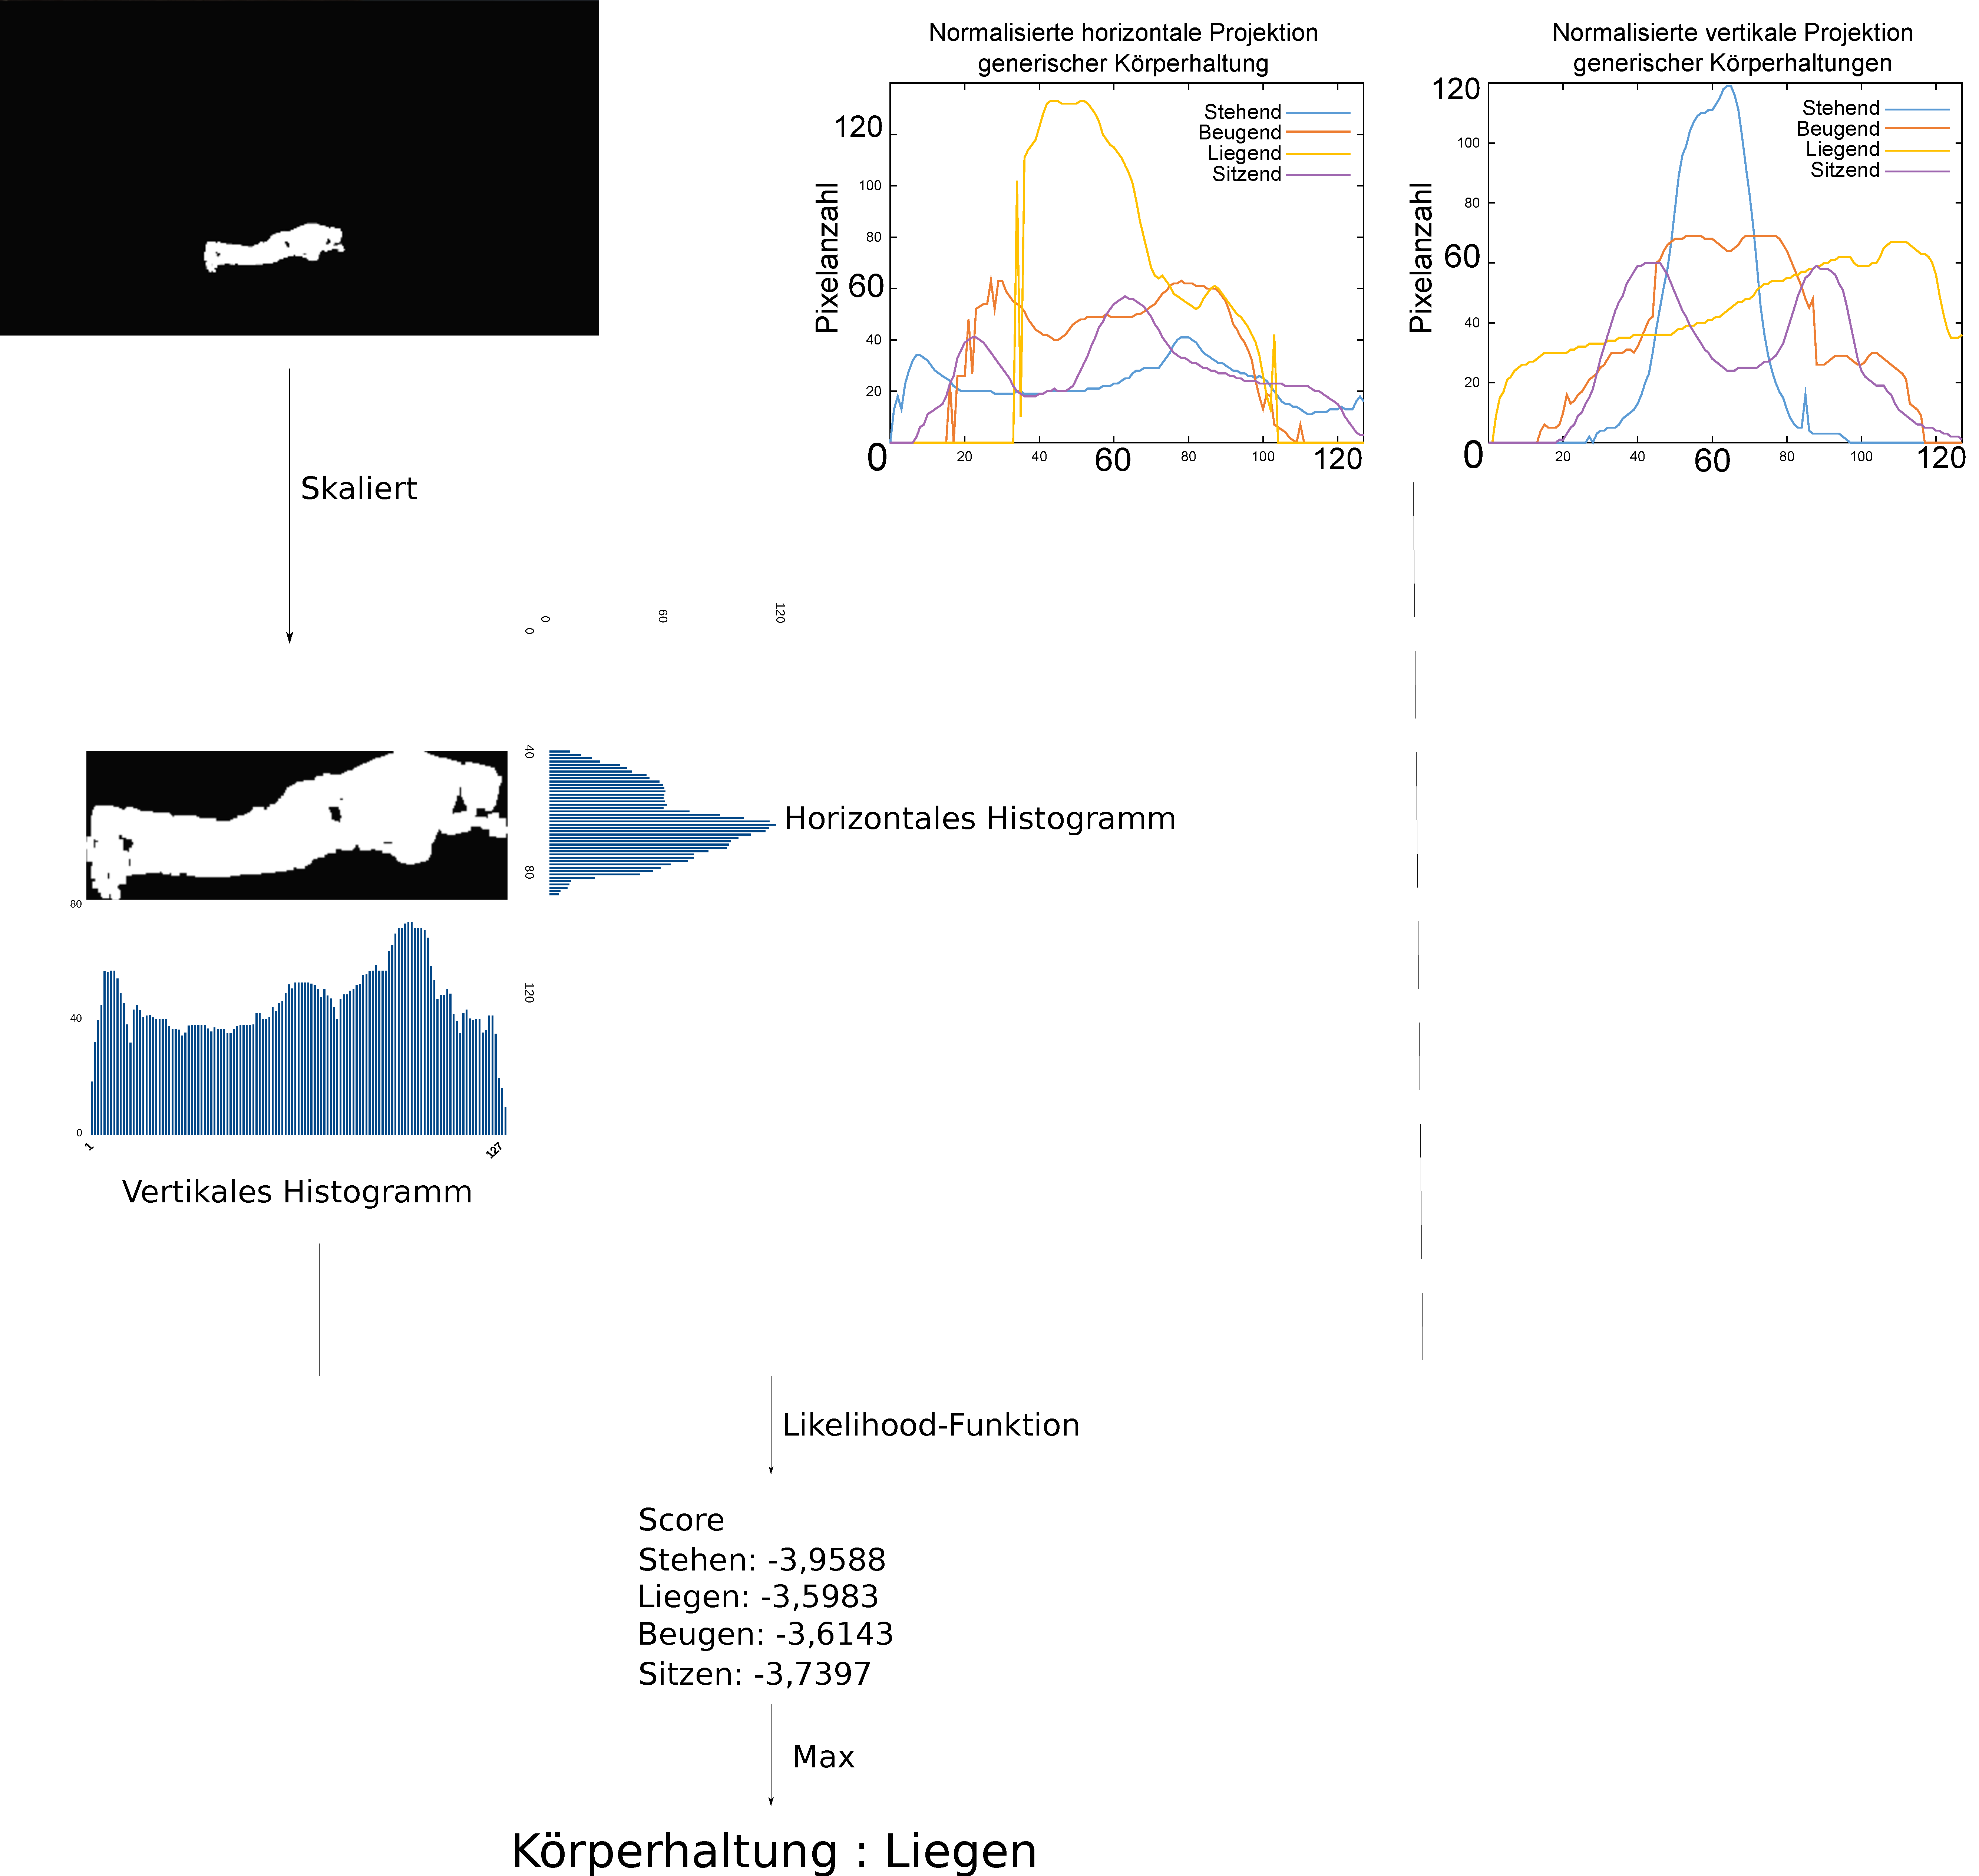
\includegraphics[width=1\textwidth]{fig/schatzung2.pdf}
	\caption{Beispiel f�r einen Prozess von Sch�tzung einer Silhouette beim Liegen.}
	\label{fig:schatzung2}
\end{figure}

\begin{figure}[H]
	\centering
	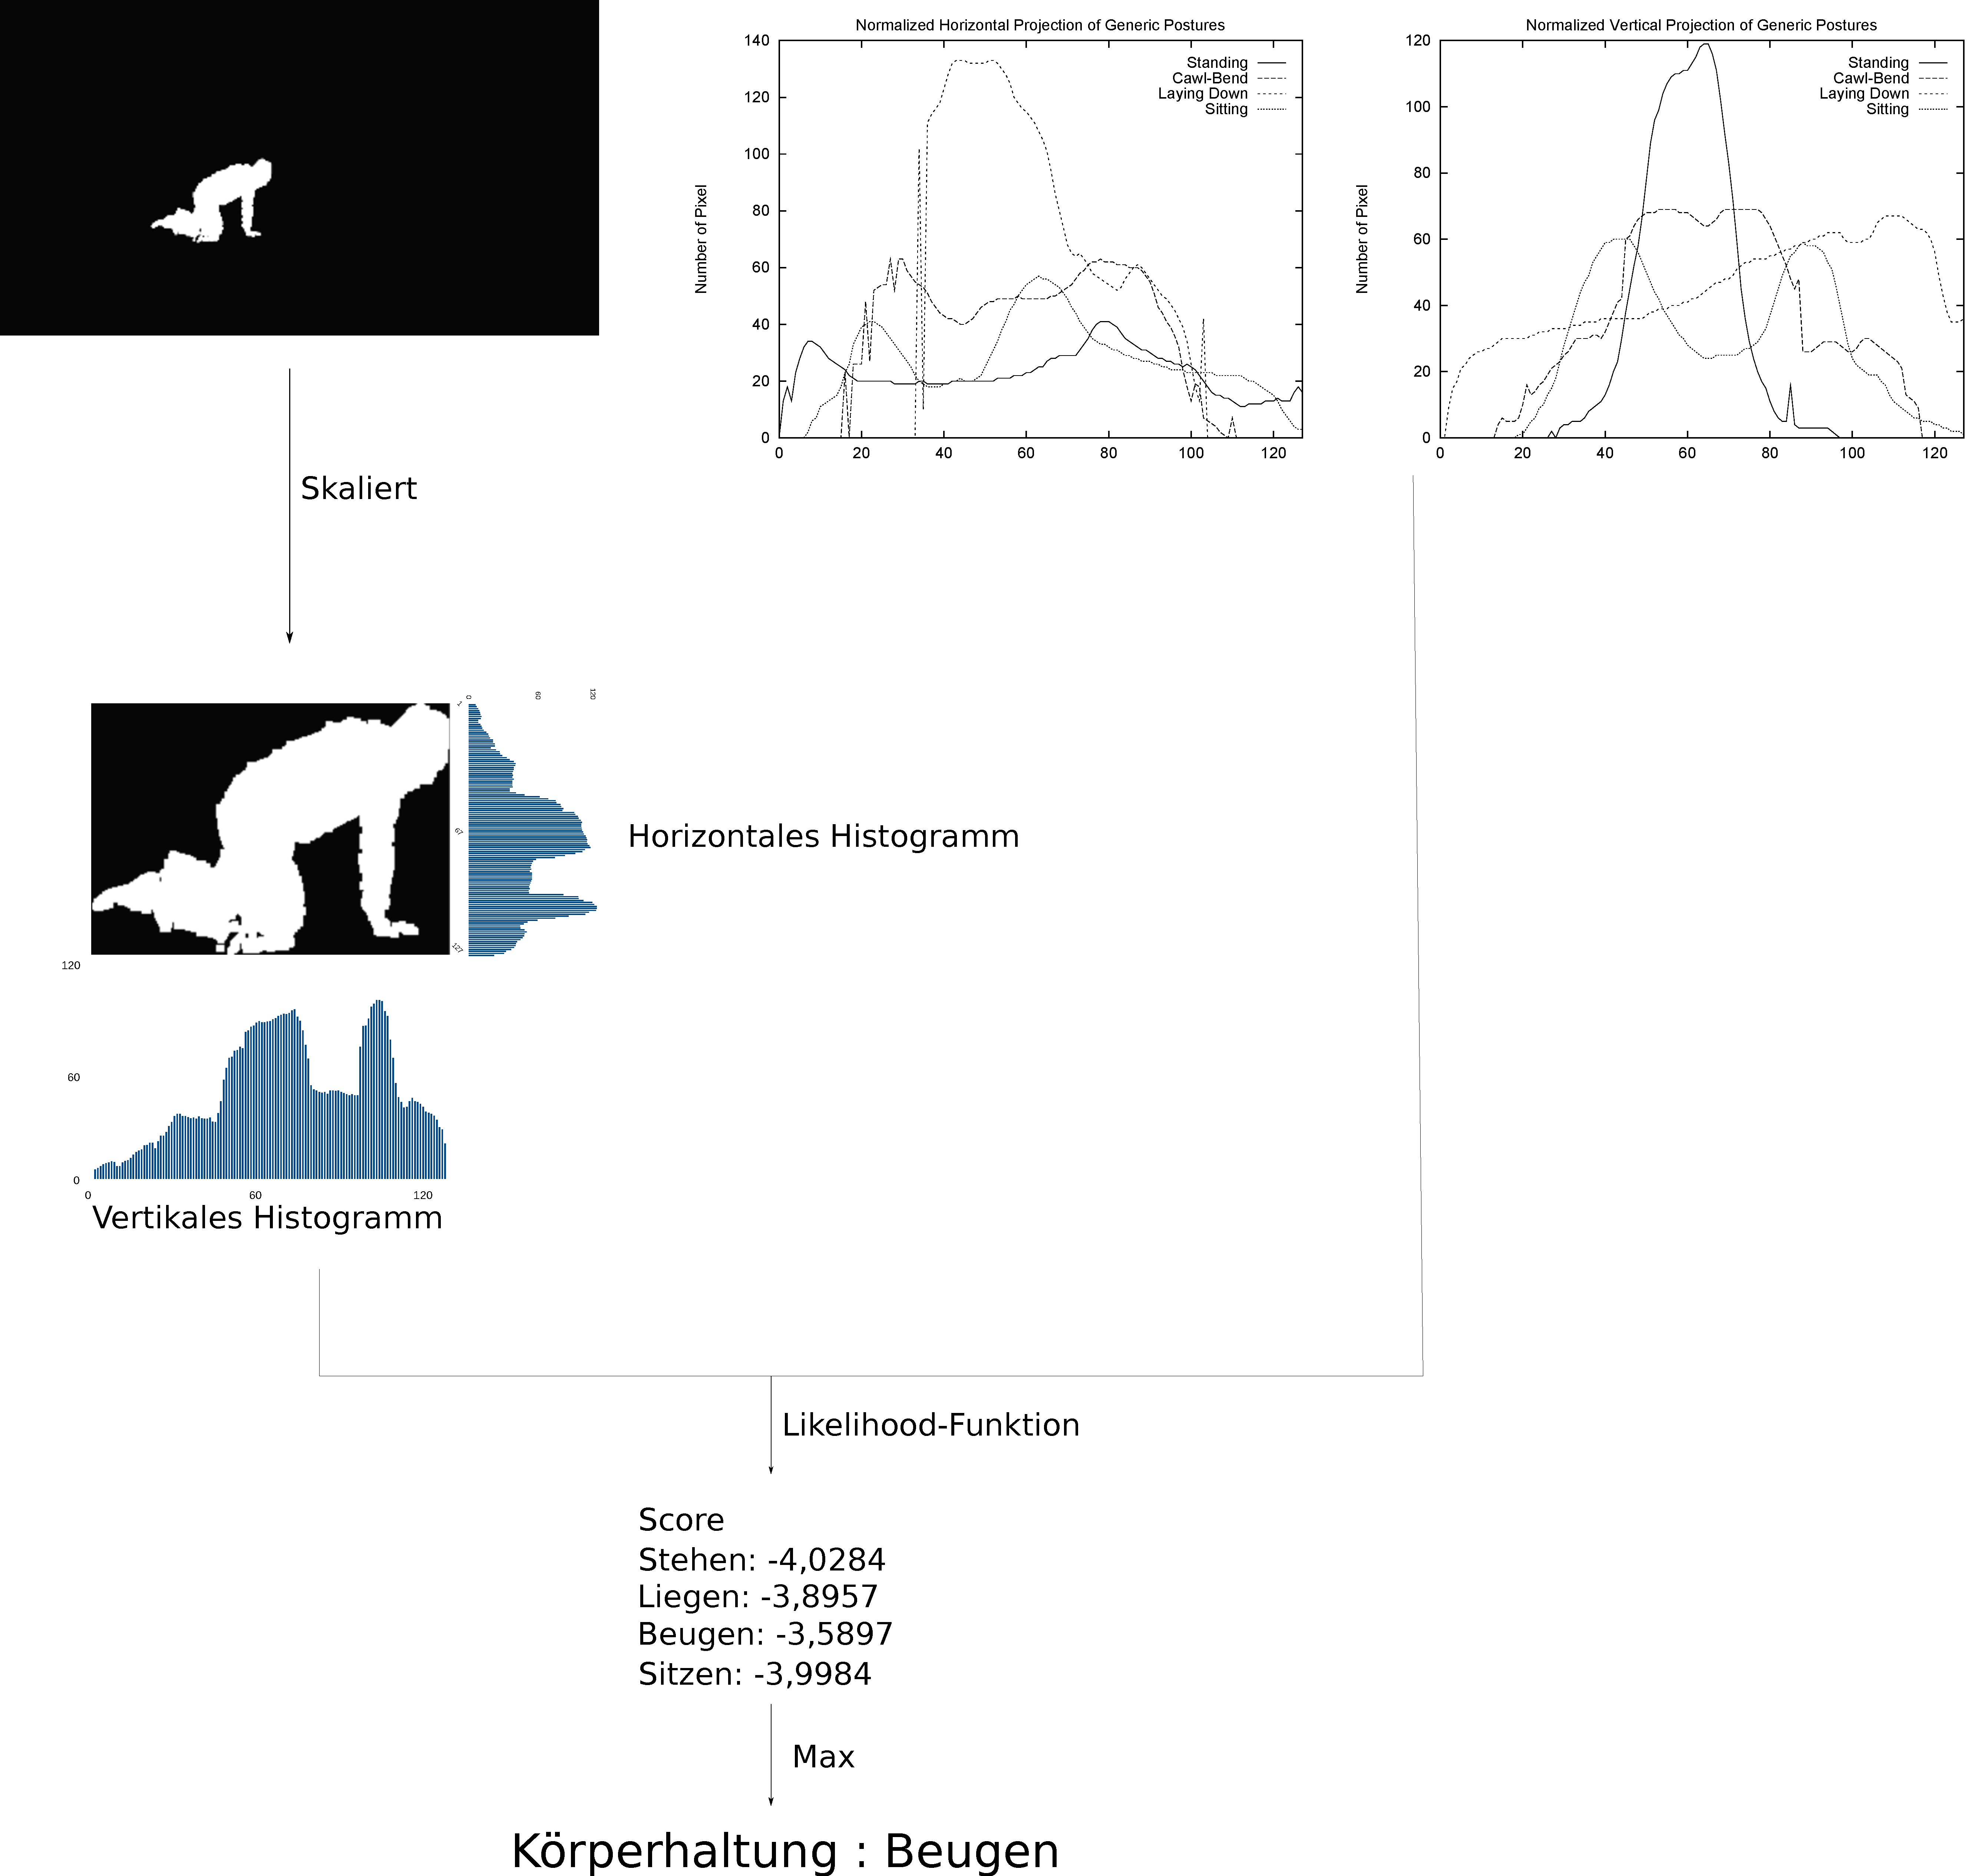
\includegraphics[width=1\textwidth]{fig/schatzung3.pdf}
	\caption{Beispiel f�r einen Prozess von Sch�tzung einer Silhouette bei Beugen.}
	\label{fig:schatzung3}
\end{figure}


Um die Zuverl�ssigkeit von diesem Verfahren zu �berpr�fen, wird die K�rperhaltung in Testvideos Bild f�r Bild annotiert, auf welchem Bild und in welcher Position in der Szene die Testperson liegt, steht, sitzt oder sich beugt. Das ergibt eine Genauigkeit von mehr als $70\%$. Die graphische Darstellung in Abbildungen \ref{fig:schatzeva} und \ref{fig:schatzeva2} zeigt das Ergebnis der Sch�tzung der K�rperhaltung. Dabei wird die K�rperhaltung als Nummer kodiert. Null steht f�r stehend, eins f�r liegend, zwei f�r beugend und drei steht f�r sitzend. Wenn die Sch�tzung minus eins ergibt, dann bedeutet das, dass sich keine sich bewegende Objekte (in diesem Fall Personen) mehr in der Szene befinden. Die blaue Gerade stellt den Referenz-Wert in den Testvideos dar und die gelbe Gerade ist das Ergebnis der Sch�tzung. Anhand der graphischen Darstellungen (siehe Abbildung \ref{fig:schatzeva} und \ref{fig:schatzeva2}) kann festgestellt werden, dass an manchen Stellen die Sch�tzung falsch lag und danach wieder richtig bewertet wurde. Das Problem tritt nur in vereinzelte Frames auf, wobei immer ein Fenster von mehreren Frames betrachtet wird und der Fehler damit nicht weiter untersucht werden muss. In Abbildung \ref{fig:schatzeva2} von Bild 700 bis 850 gibt es zwei Stellen, an denen die K�rperhaltung vom Zustand \glqq{}Stehend\grqq{} auf \glqq{}Sitzend\grqq{} oder \glqq{}Beugend\grqq{} falsch bewertet wurden. Weil der Fokus in dieser Arbeit nicht speziell auf Sch�tzung der K�rperhaltung sondern auf die Erkennung der au�ergew�hnlichen Situationen ist, kann das Problem mit den minimalen falschen Erkennungen im Graph vernachl�ssigt werden.

\begin{figure}[H]
	\centering
	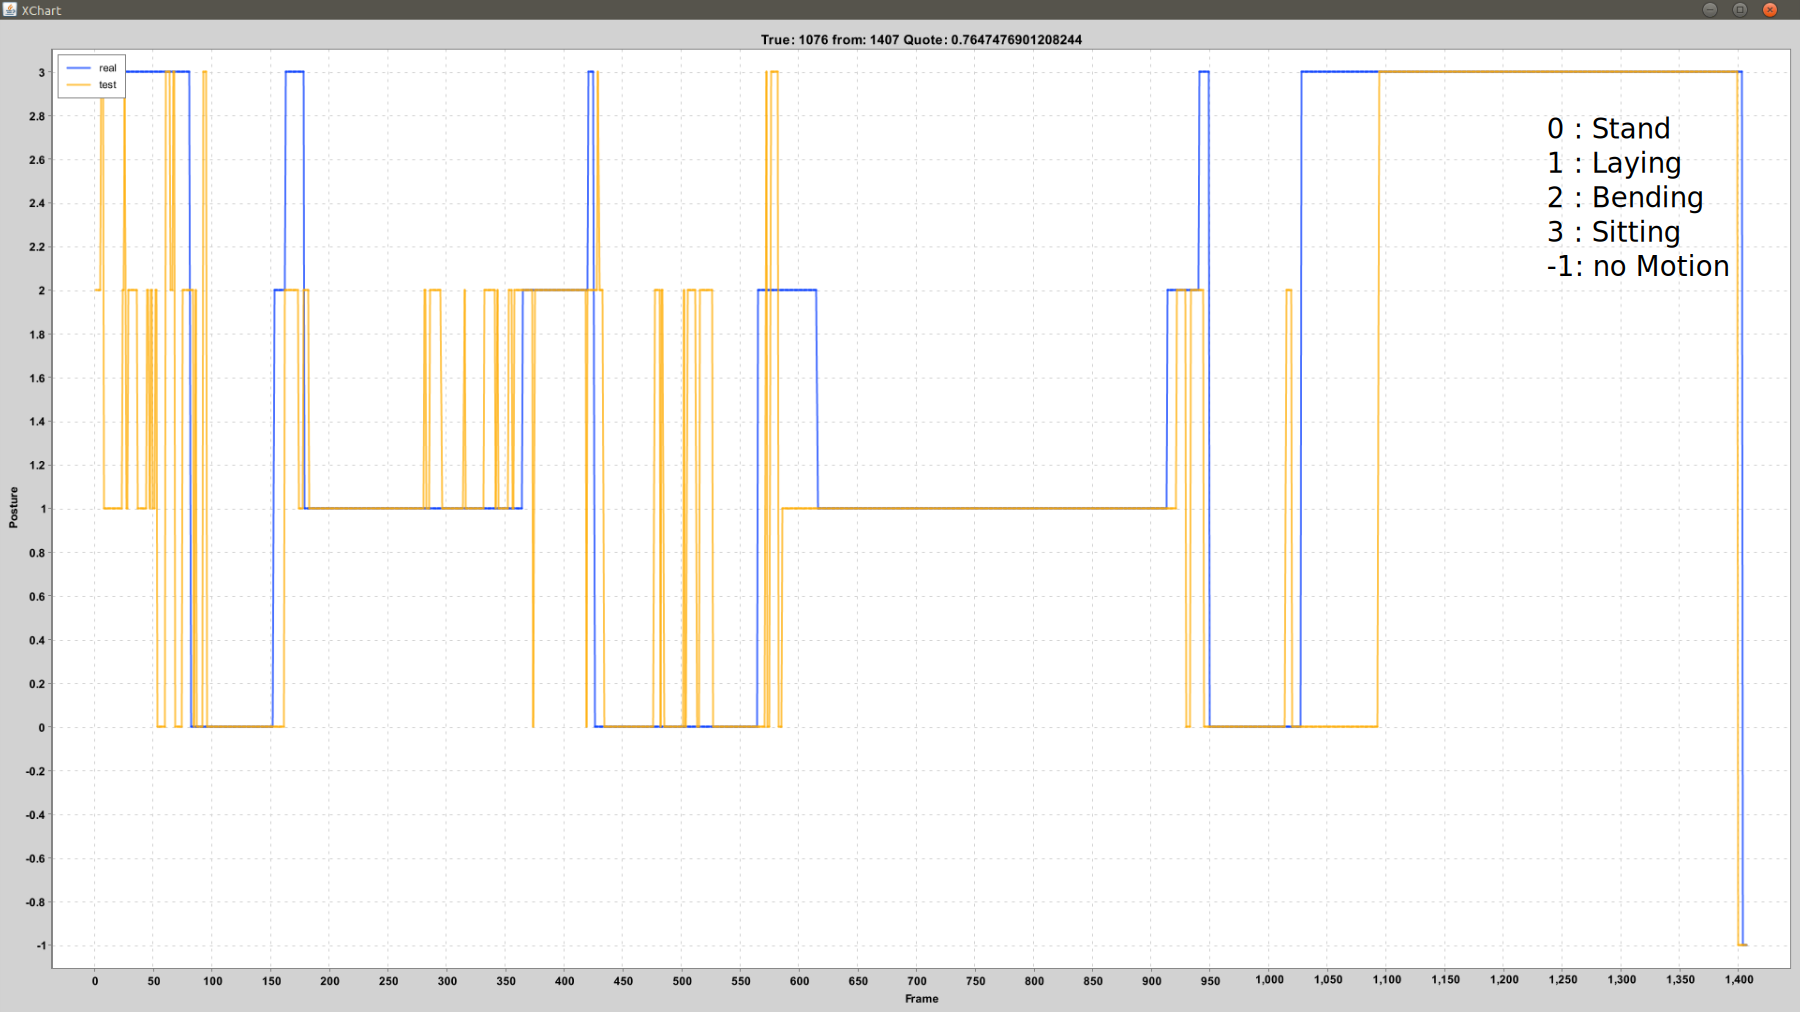
\includegraphics[width=1\textwidth]{fig/schatzungevaluation.pdf}
	\caption{�berpr�fung der Sch�tzung der K�rperhaltung am Testvideo \glqq{}fallen2.mp4\grqq{}. Die x-Achse stellt die Framenummer dar und die y-Achse ziegt die Indexe der K�rperhaltung. Die blaue Gerade ist die Referenz-K�rperhaltung und die gelbe Gerade ist die gesch�tzte K�rperhaltung. Die Sch�tzung der K�rperhaltung hat in diesem Beispiel eine Genauigkeit von 76,47\%.} 
	\label{fig:schatzeva}
\end{figure}

\begin{figure}[H]
	\centering
	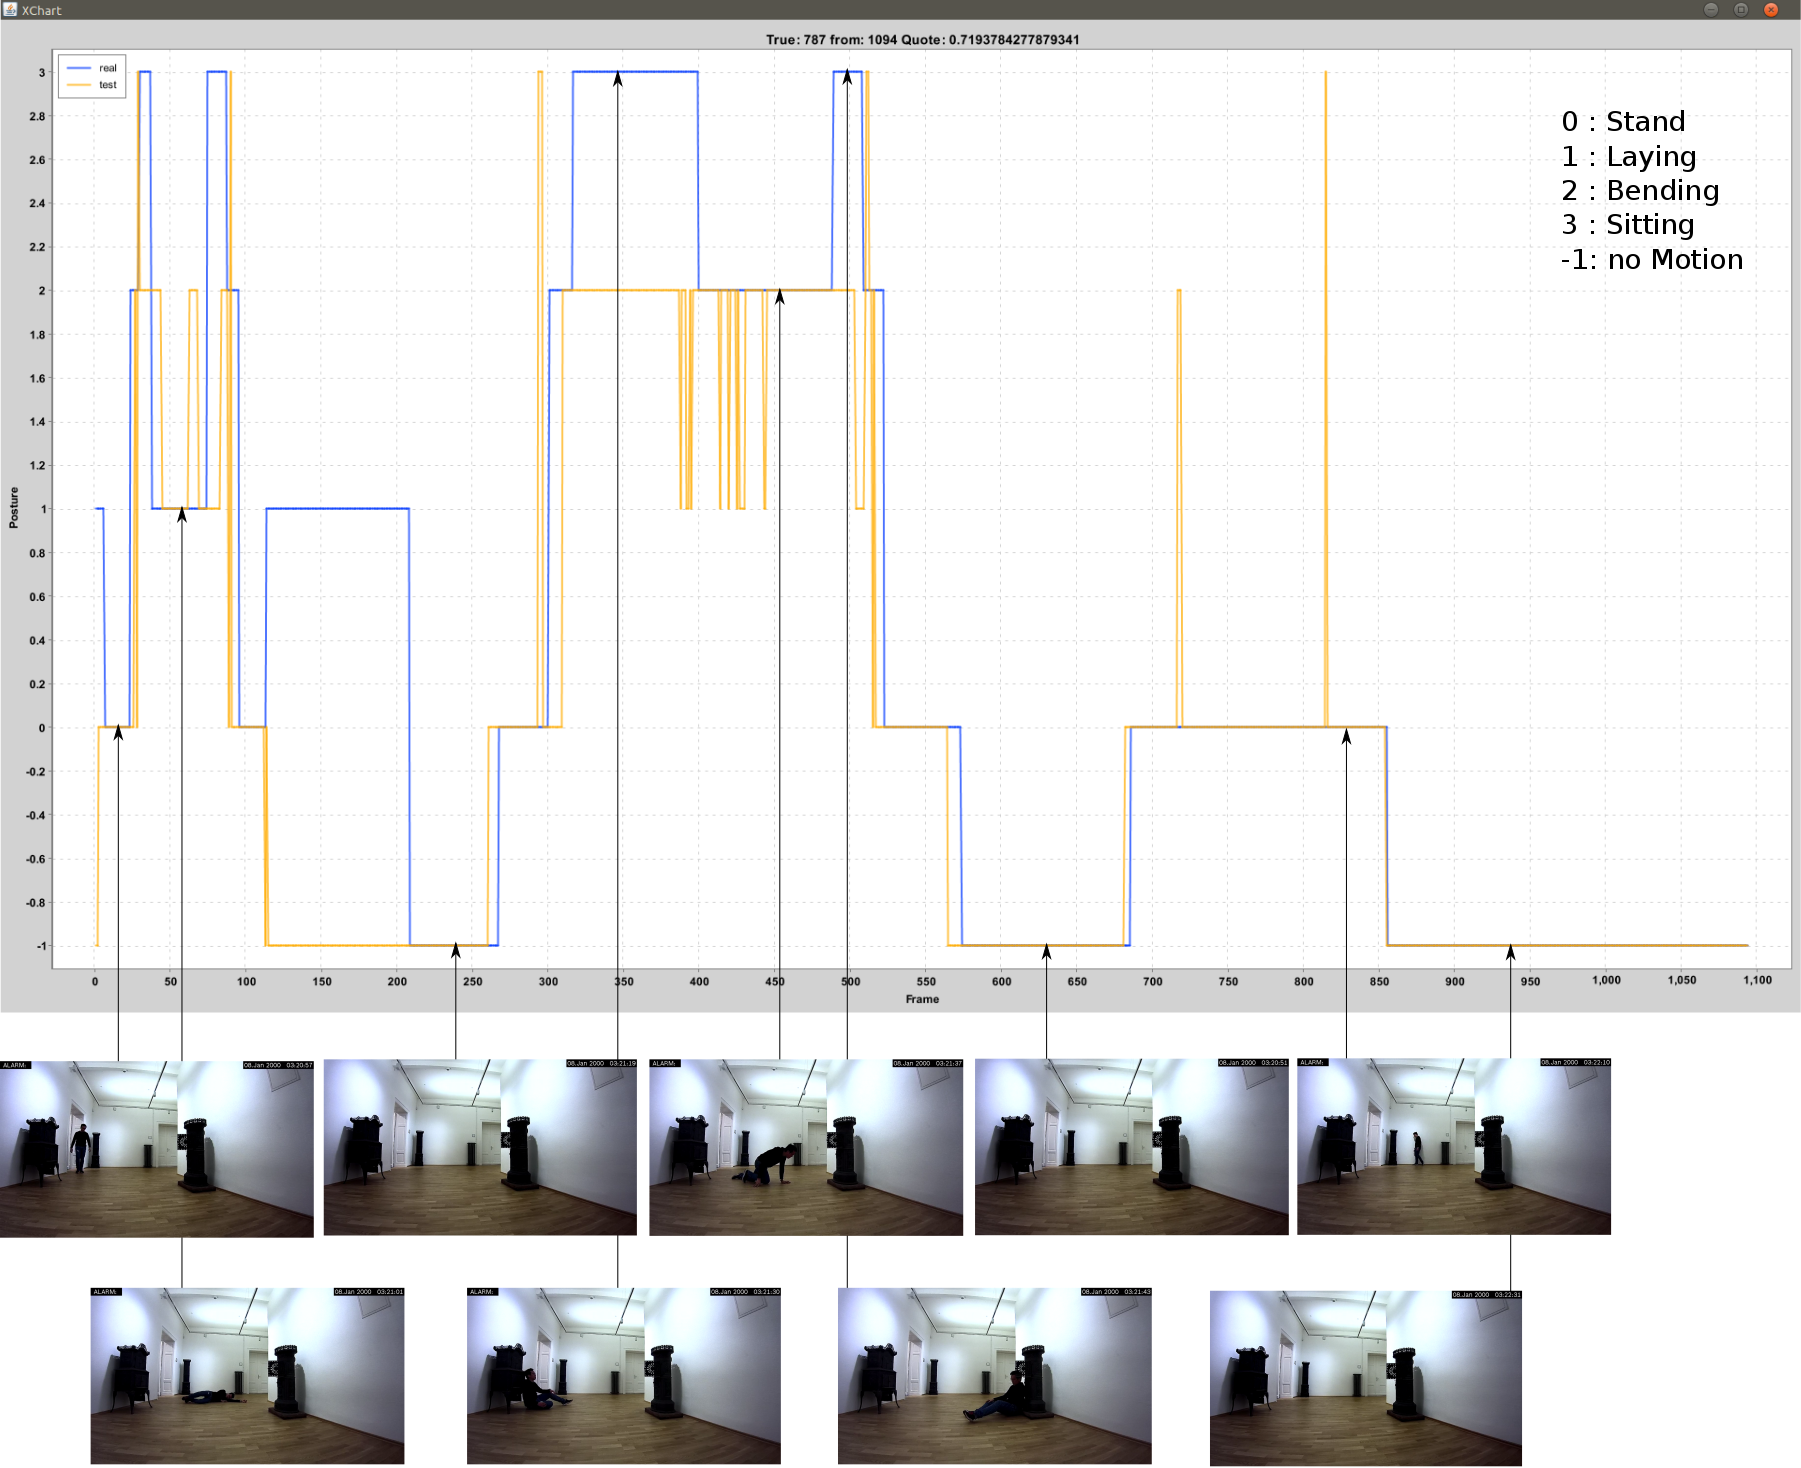
\includegraphics[width=1\textwidth]{fig/schatzungevaluation2.pdf}
	\caption{�berpr�fung der Sch�tzung der K�rperhaltung an \glqq{}fallen2.mp4\grqq{}. Die Sch�tzung der K�rperhaltung hat in diesem Beispiel eine Genauigkeit von 71,93\%.} 
	\label{fig:schatzeva2}
\end{figure}

\section{Erkennung au�ergew�hnlicher Situationen}
Im Abschnitt \ref{chp:BackgroundSubtraction} und \ref{chp:schatzung} wird eine Silhouette durch Bewegungen erstellt und eine Sch�tzung der K�rperhaltung durch die Histogrammanalyse berechnet. Zur Erkennung au�ergew�hnlicher Situationen wird noch die aktuelle Position der Person in einem bestimmten Zeitraum ber�cksichtigt. An dieser Stelle ist es wichtig, dass die Anwendung den Unterschied zwischen normalen Bewegungen im Alltag und au�ergew�hnlichen Situationen erkennt. Wenn beispielsweise die K�rperhaltung einer Person als \glqq{}Liegend\grqq{} gesch�tzt wird, kann es sein, dass die Person auf einem Sofa oder in einem Bett schl�ft. Wenn die Person im Bett liegt, handelt es sich um eine normale Situation. Deswegen ist es wichtig die Positionen der M�beln im Raum zu identifizieren. Zur Erkennung dieser Positionen sind vier Ans�tze in Betracht gezogen worden. Der erste Ansatz erfordert ein vorhandenes 3D-Modell des Raums, welches durch eine Kamera konstruiert werden kann. Diese Idee hat den Vorteil, dass die Positionen von M�beln im Raum direkt identifiziert werden k�nnen und damit schnell festgestellt wird, ob sich eine Person auf dem Boden oder im Bett liegt. Die Arbeit f�r die Erstellung des 3D-Modells ist sehr zeitaufwendig und es ist n�tig, f�r jeden neuen Raum ein neues 3D-Modell zu berechnen. Es gibt noch eine andere Techniken zur Identifizierung der Positionen von M�bel im Raum. Der zweite Ansatz betrachtet die \glqq{}Bird Eye View\grqq{}(BEV) Methode. Diese Technik wird bei Automobilen mit R�ckfahrkamera angewendet. Der Nachteil ist: BEV braucht exakt eine exakt kalibrierte Kamera und alle Parameter des Kameramodells m�ssen bekannt sein, damit eine Transformation gemacht werden kann. Au�erdem ist ein 2D-Modell der Wohnung ben�tigt, damit die M�bel in BEV erkannt werden k�nnen. Aus diesem Grund ist diese Methode f�r dieses Projekt nicht anwendbar, weil die Kamera an einer beliebigen Position im Raum aufgestellt werden kann. Der dritte Ansatz ist die neuronale Netze. Diese Methode ist h�ufig im Bereich von Objekterkennungen angewendet. Um die Objekte richtig zu erkennen, brauchen die neuronale Netze riesige Daten von Objekte. Die neuronale Netze werden anhand der Gr��e der Datenmenge bei dem Trainieren verbessert. In diesem Projekt wird ein vor-trainiertes Netz zur Erkennung der M�beln angewendet. Das vor-trainiertes Netz kann ein Sofa mit einer Wahrscheinlichkeit von 28,80\% und einen Stuhl mit einer Wahrscheinlichkeit von 25,76\% erkennen (siehe Abbildung \ref{fig:nn}). Au�erdem ist der Boden auch als ein Sofa, die Testperson als eine Katze falsch klassifiziert. Dies neuronale Netz kann mit mehrere Bilder weiter trainiert, um ein bessere Ergebnis zu liefern. Das Trainieren eines neuronalen Netzes ist aufwendig und ben�tigt eine gro�e Menge von Bildern. Die sind zwei Beschr�nkungen dieses Ansatzes. 

\begin{figure}[H]
	\centering
	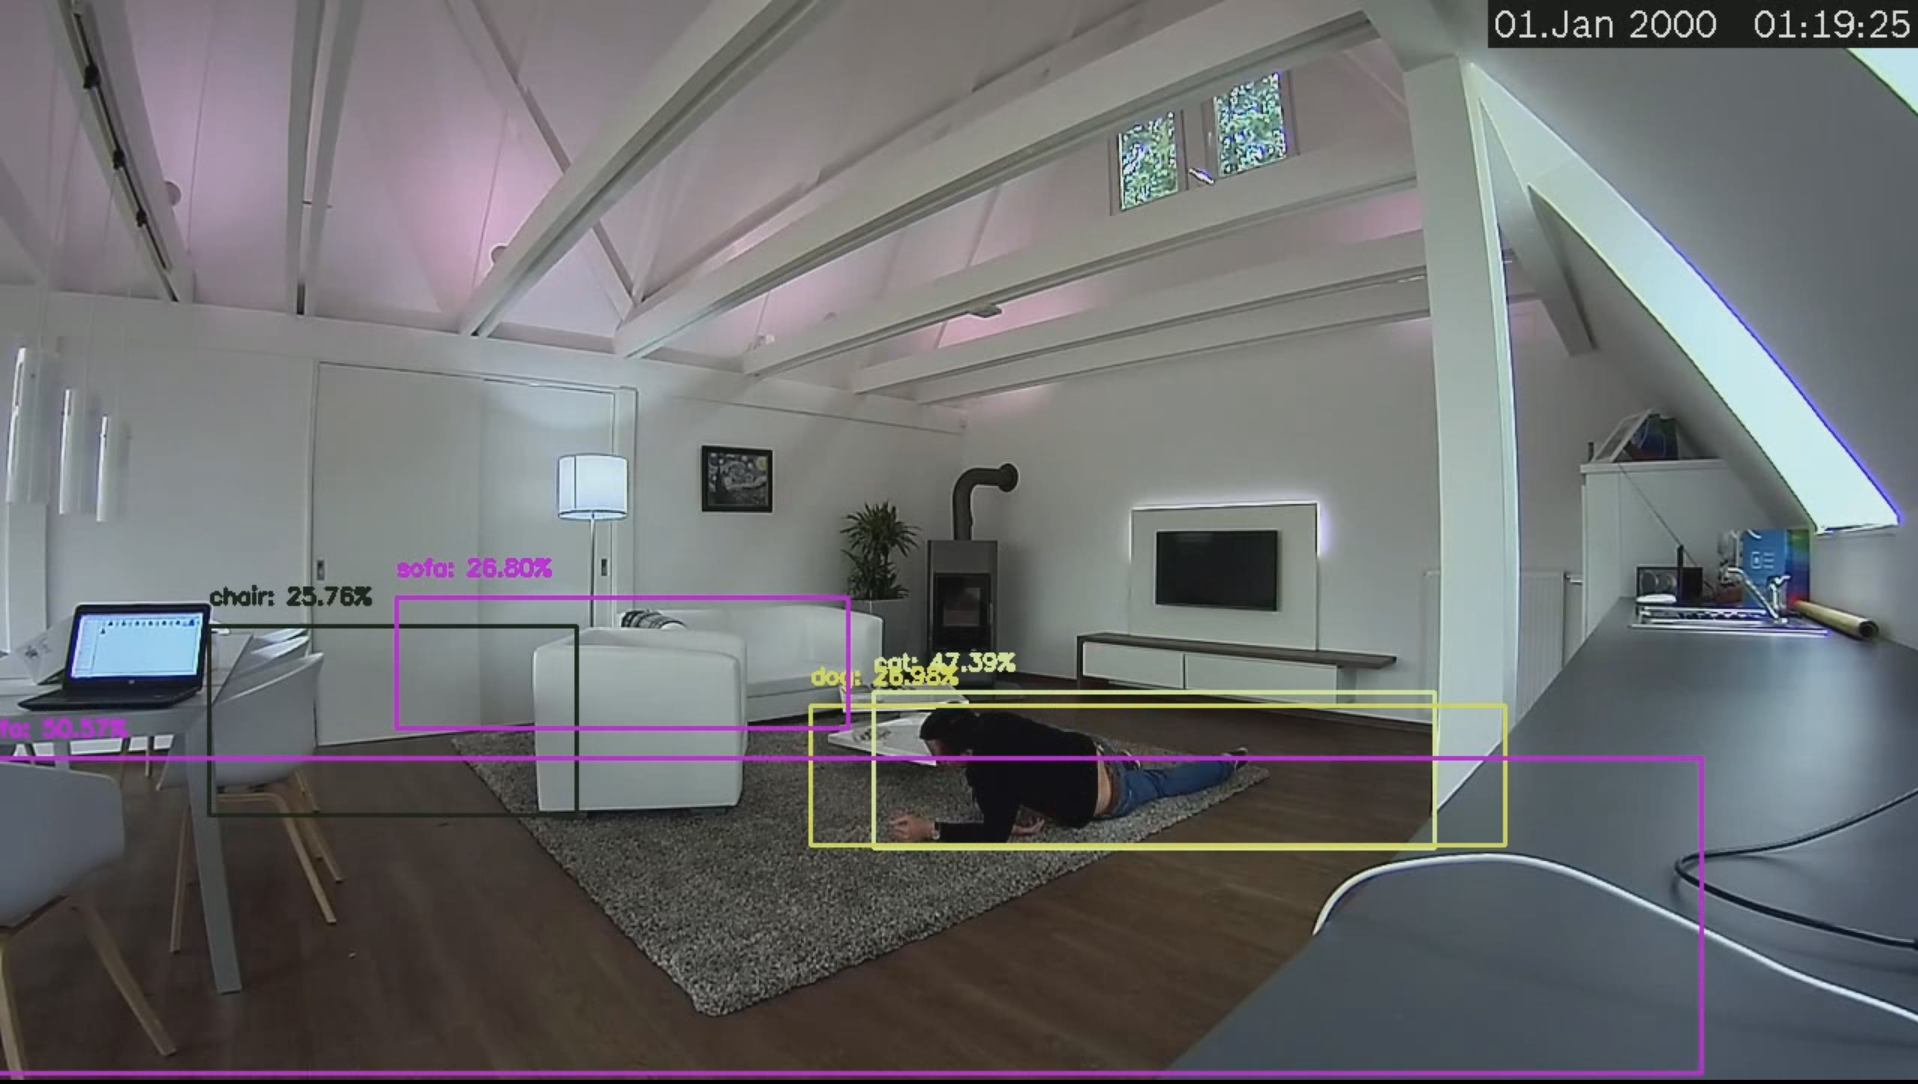
\includegraphics[width=0.95\textwidth]{fig/neurolnet.png}
	\caption{Objekterkennung mit einem neuronalen Netz.}
	\label{fig:nn}
\end{figure}

Um das Problem der Unterscheidung von normalen und abnormalen Situationen zu l�sen, wird eine logische Methode, die als Fuzzylogik genannt wird, verwendet. Dies ist der vierte Ansatz, der auch in diesem Meilenstein befolgt wurde. Die Positionen der M�beln im Raum sind auf dem Bild von Benutzern zun�chst vordefiniert. Die Fuzzylogik berechnet durch die Positionen der M�bel (zum Beispiel: Boden), die aktuelle K�rperhaltung und die aktuelle Zeit. Dann wird die Wahrscheinlichkeit ausgerechnet, ob es sich um eine au�ergew�hnliche Situation handelt. Wie in Abschnitt \ref{sec:fuzzylogik} schon erw�hnt, besteht die Fuzzylogik aus drei Schritten: Umwandlung von Eingaben in Fuzzymengen, Anwendung von vordefinierten (IF-ELSE) Regeln und Defuzzifizierung (siehe Abbildung \ref{fig:fuzzylogik}).

\begin{figure}[H]
	\centering
	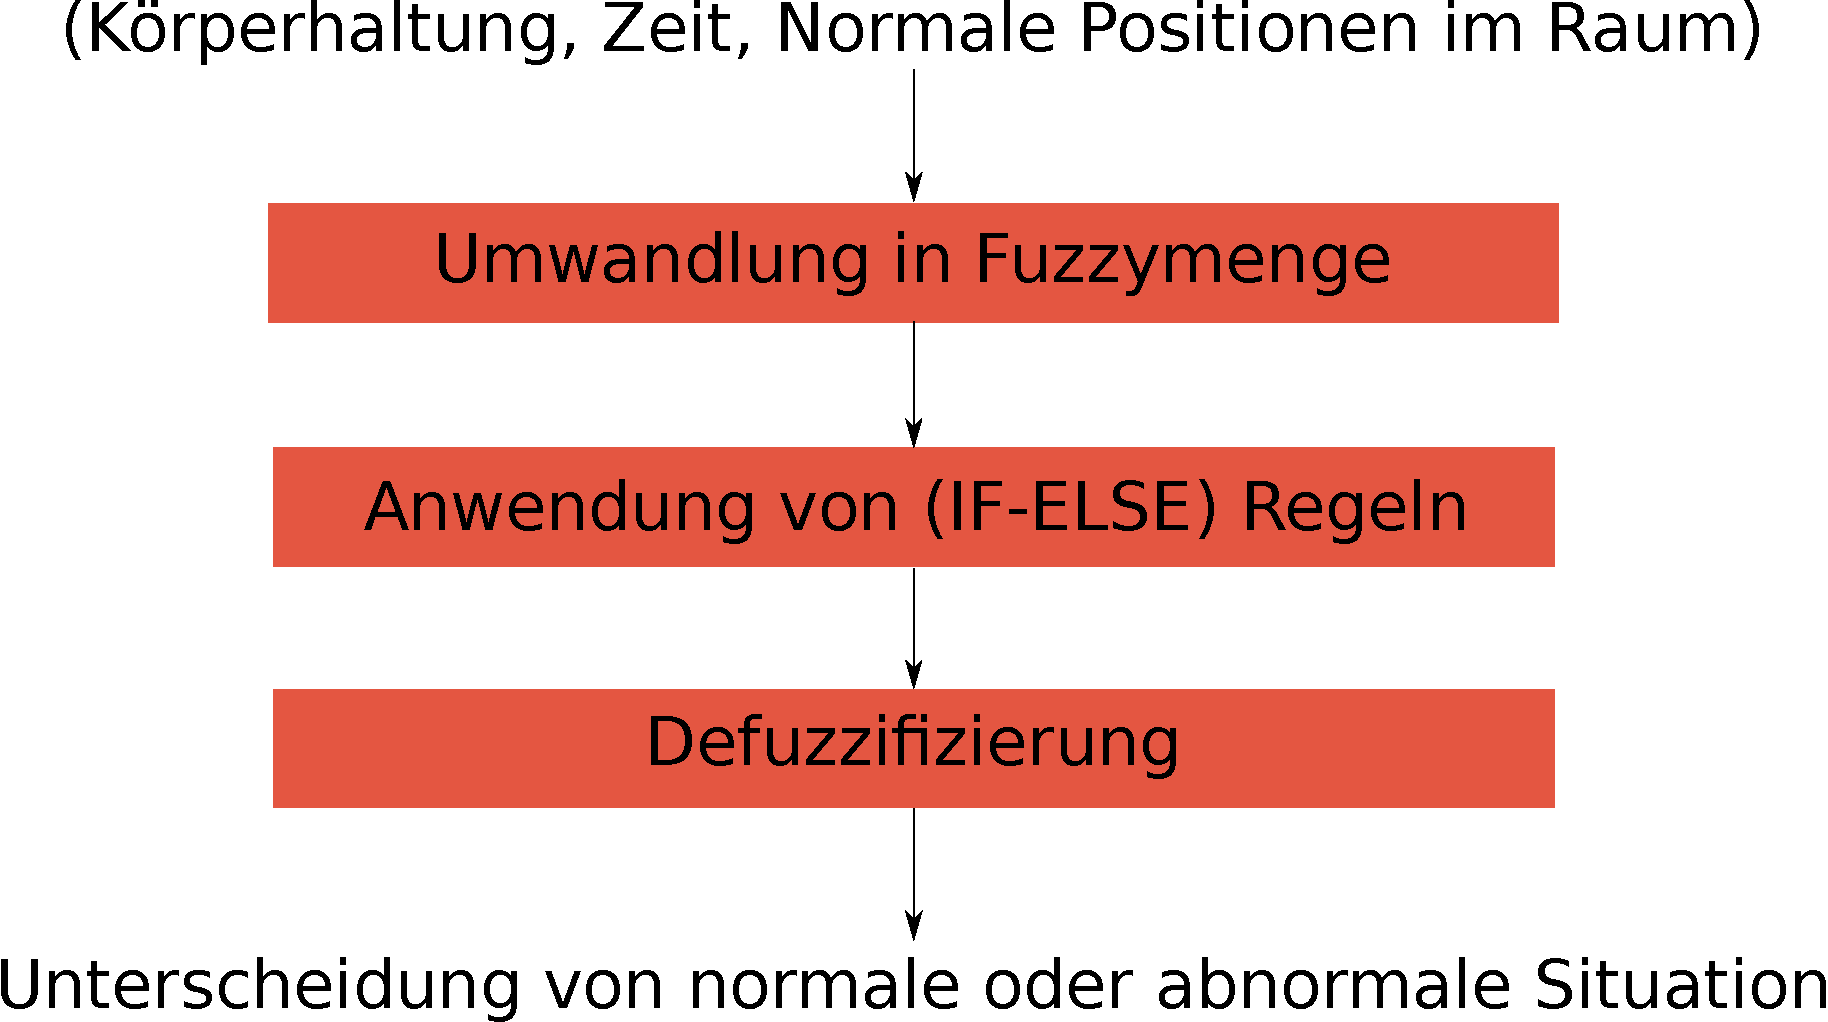
\includegraphics[width=0.85\textwidth]{fig/fuzzylogik.pdf}
	\caption{Dritter Meilenstein}
	\label{fig:fuzzylogik}
\end{figure}

Zuerst m�ssen die Mitgliederfunktionen der Eingaben definiert werden und die sind wie folgt beschrieben:

\begin{itemize}
	\item Die K�rperhaltung besteht aus vier Zust�nden: Stehend (Index: 0), Liegend (Index: 1), Beugend (Index: 2), Sitzend (Index: 3). Diese sind als Punkte im Fuzzymodel definiert (siehe Abbildung \ref{fig:fuzzyfunktion}a).
	\item Die Zeit besteht aus Tag und Nacht und ist mit glockenf�rmige Funktionen mit Parametern $a=6$, $b=10$ mit $mean=14$ f�r Tag und $mean=2$ f�r Nacht definiert (siehe Abbildung \ref{fig:fuzzyfunktion}b). Der Wertbereich f�r die Zeit ist ein Intervall $[0, 24]$ f�r $24$ Stunden am Tag. Diese Funktion kann wie folgt beschrieben werden\cite{rosenfeld1971fuzzy}:
	\begin{equation}
	f(a, b, mean) = \frac{1}{1 + |\frac{x - mean}{a}|^{2b}}
	\end{equation} 
	\item Die normalen Koordinaten im Raum sind die Positionen, an denen die Testperson normalerweise liegt, sitzt oder steht. Diese wird mit Gau�schen-Funktionen definiert, wobei die Mittelwerte der Funktion $xy$-Koordinaten sind und die Standardabweichung $\sigma = 30$ Pixel betr�gt (siehe Abbildungen \ref{fig:fuzzyfunktion}c und \ref{fig:fuzzyfunktion}d). Dies entspricht der Gr��e eines 1,5m lang Sofas mit einem Abstand 3m von der Kamera. Der Wertbereich f�r die x-Koordinate ist ein Intervall [0, Breite des Bildes] und f�r y-Koordinate ist ein Intervall [0, H�he des Bildes].
	\item Die Ausgabe ist der \glqq{}Status\grqq{}. Dieser besteht aus den Komponenten \glqq{}good\grqq{} und \glqq{}bad\grqq{}, welche als Fuzzymenge zusammengef�hrt werden. Die Komponente \glqq{}good\grqq{} steht dabei f�r die Wahrscheinlichkeit, dass es sich um eine normale Situation und \glqq{}bad\grqq{} gibt die Wahrscheinlichkeit an, dass es sich um eine au�ergew�hnliche Situation handelt. Der \glqq{}Status\grqq{} besitzt damit zwei Gau�sche-Funktionen mit je Standardabweichung $\sigma = 1$ mit Mittelwert $\mu=4$ f�r abnormale und $\mu=6$ f�r normale Situationen (siehe Abbildungen \ref{fig:fuzzy1}, \ref{fig:fuzzy2}).
\end{itemize}  

Die oben vordefinierten Mitgliederfunktionen werden in der Abbildung \ref{fig:fuzzyfunktion} graphisch dargestellt. Zur Anwendung von (IF-ELSE) Regeln (siehe Algorithmus \ref{algo:fuzzy_modell}) wird das Minimum als Aktivations-Methode und das Maximum als Akkumulations-Methode eingesetzt. Die Regeln im Algorithmus \ref{algo:fuzzy_modell} k�nnen wie folgt interpretiert werden:

\begin{itemize}
	\item Es ist \glqq{}bad\grqq{}, wenn die Person nicht auf dem Sofa liegt.
	\item Es ist \glqq{}good\grqq{}, wenn die Person auf dem Sofa liegt.
	\item Es ist \glqq{}bad\grqq{}, wenn die Person am Tag liegt.
	\item Es ist \glqq{}good\grqq{}, wenn die Person am Tag steht.
	\item Es \glqq{}bad\grqq{}, wenn die Person am Tag sitzt oder sich beugt.
\end{itemize}

Bei Defuzzifizierung, die eine Abbildung der Ausgabe in eine scharfe Mengen durchf�hrt, wird die Schwerpunktmethode verwendet. Die oben vordefinierten Parameter k�nnen anhand des Raums und biologischer Uhr der Testperson angepasst werden. Zum Beispiel gibt es in einem Raum nicht nur ein Sofa sondern auch ein Bett, dann m�ssen die Koordinaten des Bettes noch definiert werden. Das hilft dem Programm zu erkennen, ob eine Person im Bett und nicht auf dem Boden ist. Die Anpassung der Parameter kann durch maschinelles Lernen nach dem Gebrauch des Benutzers verbessert werden.\\

Die Fuzzylogik berechnet, wie hoch die Wahrscheinlichkeit ist, dass sich die aktuelle Situation um eine normale Situation handelt. F�r komplexe Anwendungsf�lle wurden Gau�sche-Funktionen benutzt, um eine Demo-Software zu realisieren. Es wurde angenommen, dass die Koordinaten von einem Sofa im Raum $(591, 441)$, die aktuelle Zeit $0$ Uhr nachts und $8$ Uhr morgens sind und dass die Testperson an der Position (574, 424) liegt (Wie in die Fuzzymenge in Abbildung \ref{fig:fuzzyfunktion} eingetragen). In dem ersten Testfall, indem die Testperson nachts auf dem Sofa lag, ergab sich die Wahrscheinlichkeit $good$=93,29\%, dass es sich um eine normale Situation handelt. F�r eine au�ergew�hnliche Situation wurde eine Wahrscheinlichkeit von $bad$=26,59\% berechnet (Abbildung \ref{fig:fuzzy1}). In Regeln \ref{algo:fuzzy_modell} gibt es einen gemischten Fall, wobei die Testperson auf dem Sofa um $8$ Uhr Morgen liegt. Hier ist es gut, wenn die Person auf dem Sofa und nicht auf dem Boden liegt und schlecht, dass die Person morgens auf dem Sofa liegt. Daf�r ergab die Rechnung eine Wahrscheinlichkeit von $good$=71,6\% f�r eine normale Situation und $bad$=49,71\% f�r eine abnormale Situation (Abbildung \ref{fig:fuzzy2}). Eine Situation wird genau dann als schlechte Situation klassifiziert, wenn gilt: $bad \geq 80\%$ und $bad > good$. Diese Bedingungen k�nnen wie folgt definiert werden:
\begin{eqnarray}
\texttt{Situation schlecht} &\Leftrightarrow& bad \geq 80\% \wedge bad > good \\
\texttt{Situation gut} &\Leftrightarrow& bad < 80\% \vee bad <= good
\end{eqnarray}

\begin{algorithm}[H]
	\caption{Regeln f�r die Auswertung einer Situation}
	\label{algo:fuzzy_modell}
	\If{(posture IS laying) AND ((NOT xposition IS good) OR (NOT yposition IS good))}{status IS bad;}
	\If{(posture IS laying) AND (xposition IS good) AND (yposition IS good)}{status IS good;}
	\If{(posture IS laying) AND (time IS day)}{status IS bad;}
	\If{(posture IS standing) AND (time IS day)}{status IS good;}
	\If{((IF posture IS sitting) OR (posture IS bending)) AND (time IS night)}{status IS bad;}
\end{algorithm}

\begin{figure}[H]
	\centering
	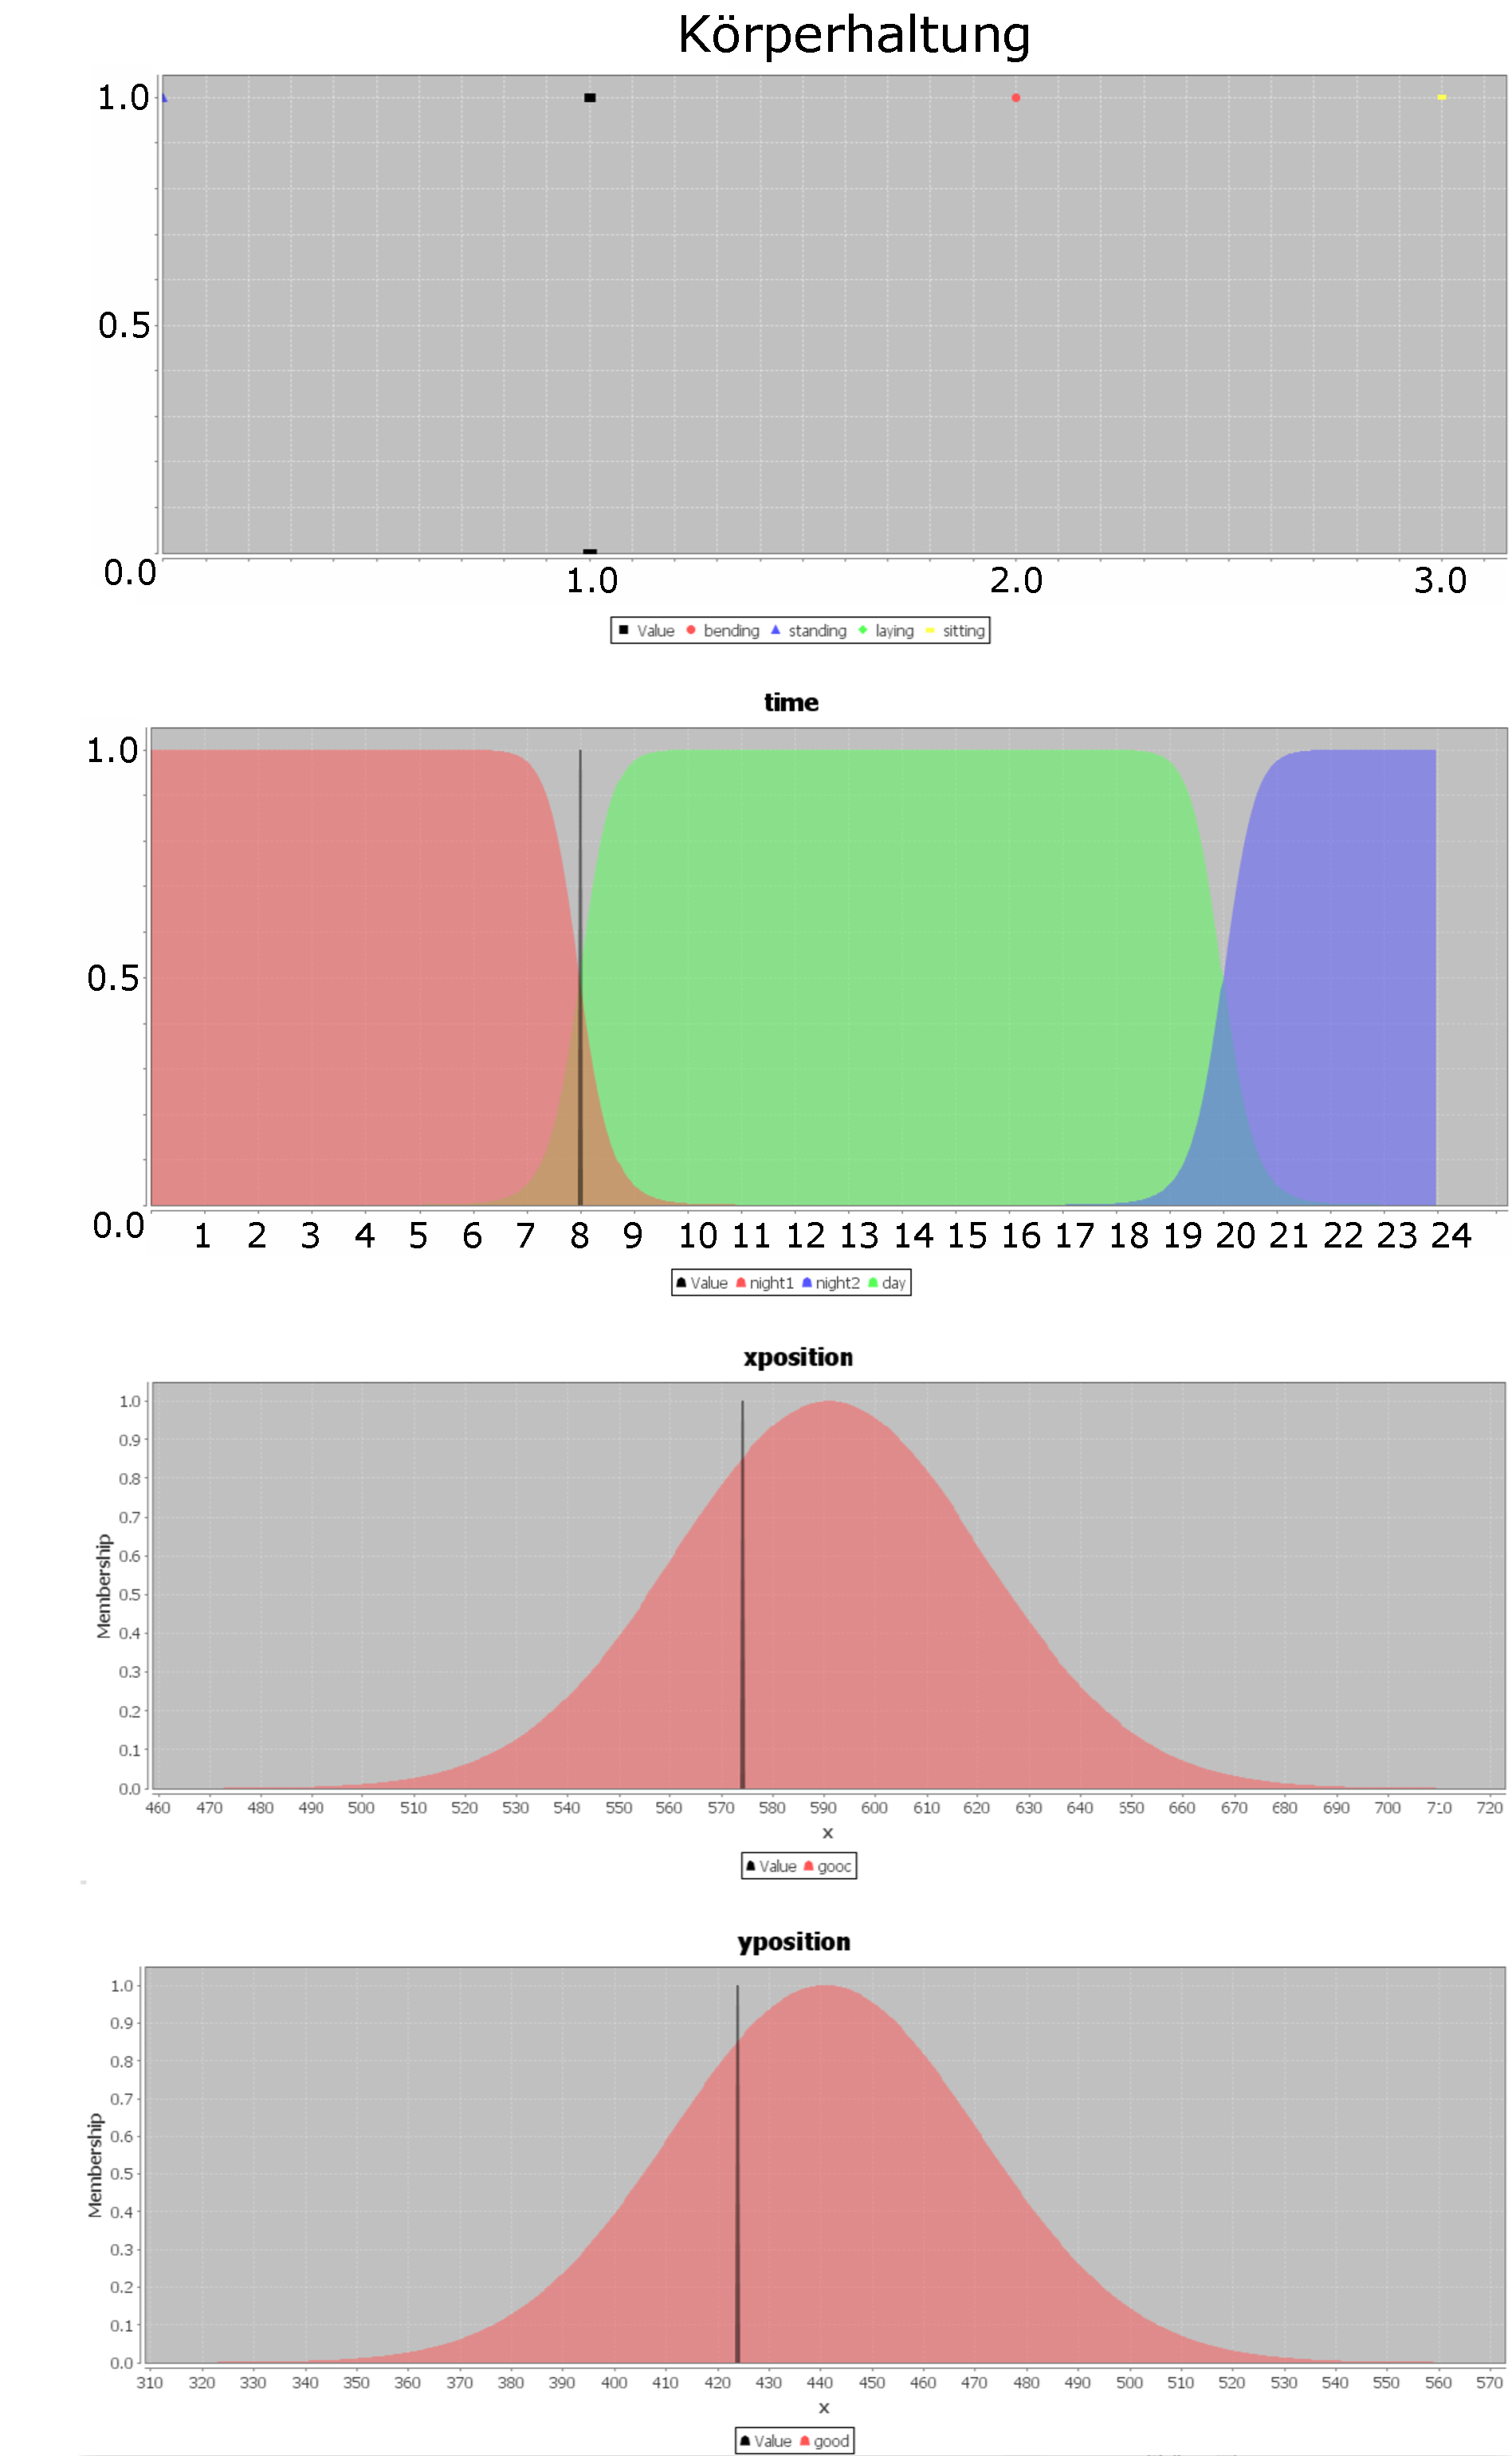
\includegraphics[width=0.75\textwidth]{fig/fuzzyfunktion.pdf}
	\caption{Die Mitgliederfunktionen der K�rperhaltung, Zeit und aktuelle Position der Person. Der Eingabebereich der Zeit ist von 0 bis 24 Uhr beschr�nkt und die Eingabe der Position muss ein positiver Wert sein. Diese Abbildung stellt ein Beispiel dar, wobei eine Person um 8 Uhr auf dem Sofa (x=574, y=424) liegt.} 
	\label{fig:fuzzyfunktion}
\end{figure}

\begin{figure}[H]
	\centering
	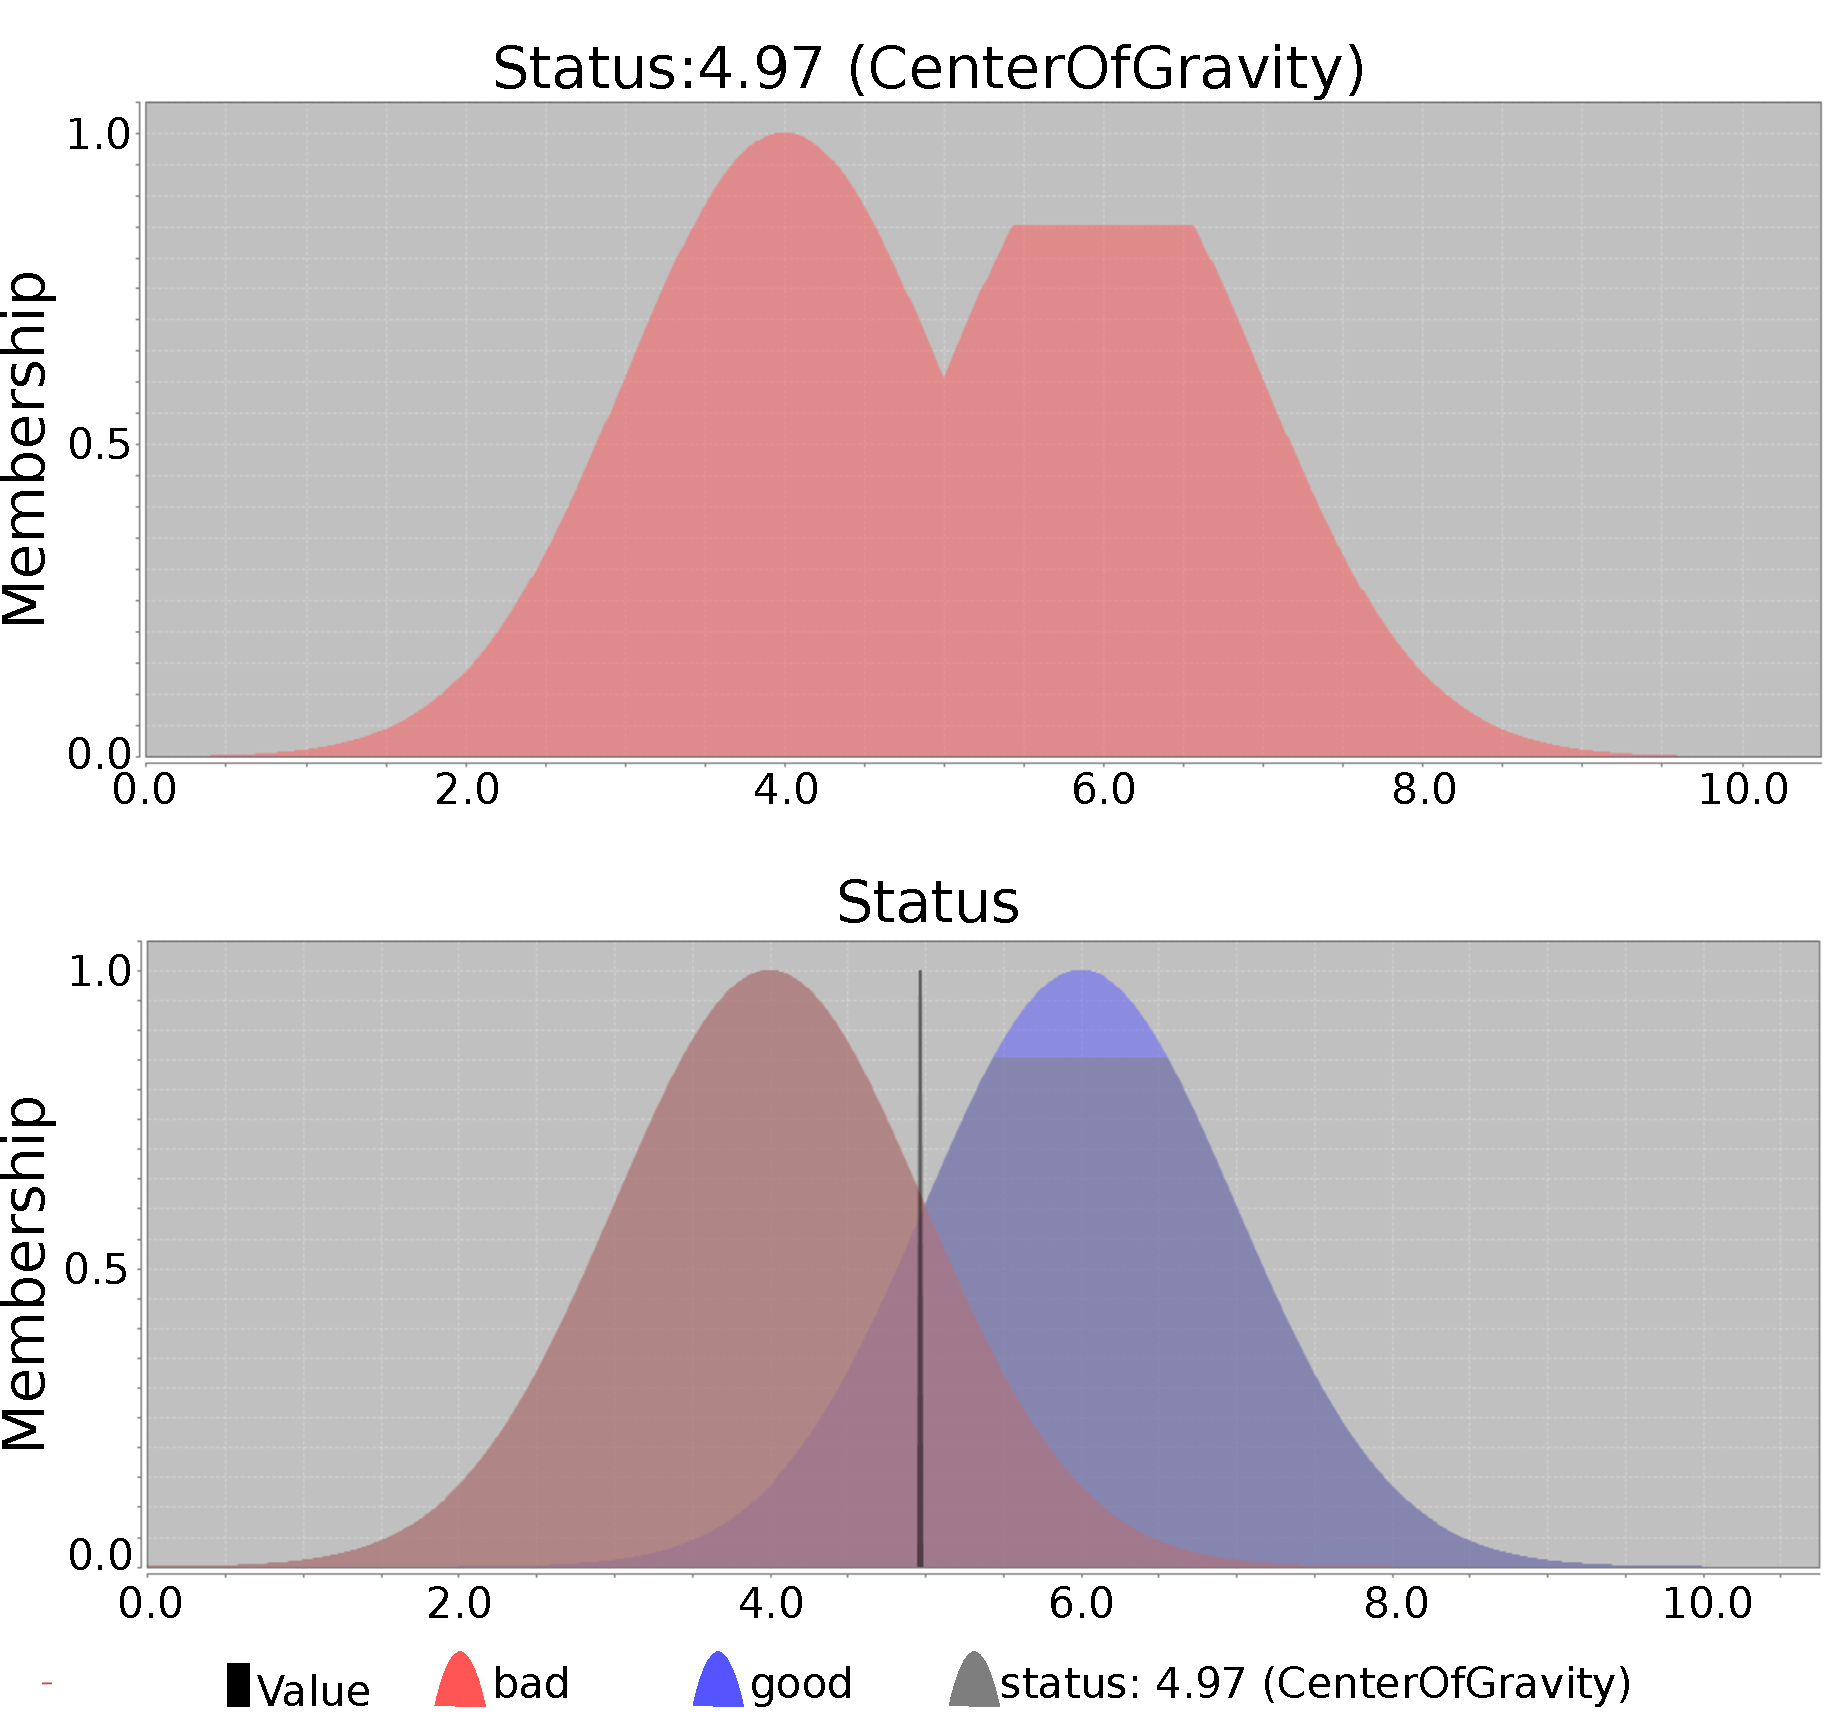
\includegraphics[width=0.59\textwidth]{fig/fuzzy1.pdf}
	\caption{Testfall: Person liegt auf dem Sofa um 12 Uhr Nachts. Das Programm liefert ein Ergebnis von 93,29\% f�r normale und 26,59\% f�r abnormale Situation.} 
	\label{fig:fuzzy1}
\end{figure}

\begin{figure}[H]
	\centering
	\includegraphics[width=0.59\textwidth]{fig/fuzzy2.pdf}
	\caption{Testfall: Person liegt auf dem Sofa um 8 Uhr Morgens. Das Programm liefert ein Ergebnis von 71,6\% f�r normale und 49,71\% f�r abnormale Situation.} 
	\label{fig:fuzzy2}
\end{figure}

Bis jetzt k�nnen die au�ergew�hnlichen Situationen von normalen Bewegungen im Alltag mit Hilfe von Fuzzylogik unterschieden werden. Die au�ergew�hnlichen Situationen sollen nicht nur in einem Bild sondern in einer Sequenz von mehreren Bildern beachtet werden, damit das System bessere Entscheidungen f�r eine abnormale Situation treffen kann. Wenn immer nur ein Bild beachtet wird, k�nnte eine falsch klassifizierte Situation in nur einem Bild bereits einen Alarm ausl�sen. Um die Beobachtung in mehreren Bildern zu realisieren, wird ein Modell gebaut, wobei die erkannte Person in einer Begrenzungsbox in einem Zeitraum betrachtet wird. Das hei�t, jedes \inlinecode{C++}{Personen}-Objekt besteht aus einer aktuellen Begrenzungsbox $B_{current}$, die nach der Hintergrundsubtraktion erstellt wird. Nach jedem eingegangenen Bild wird die neue Begrenzungsbox $B_{new}$ mit der aktuellen Begrenzungsbox $B_{current}$ verglichen, um zu bestimmen, ob es sich um die selbe Person handelt und ob die Person sich bewegt hat. Eine globale Variable \inlinecode{C++}{movementMaximum} gibt die maximale zul�ssige Geschwindigkeit an, mit der sich eine Person bewegen kann. Der euklidische  Abstand zwischen $B_{current}$ und $B_{new}$ wird berechnet und mit der \inlinecode{C++}{movementMaximum} verglichen. Wenn dieser euklidische Abstand gr��er als \inlinecode{C++}{movementMaximum} ist, wird eine neue Person erstellt und die aktuelle Person wird ignoriert. Wenn dieser Abstand kleiner oder gleich  \inlinecode{C++}{movementMaximum} ist, wird $B_{current}$ der Person mit $B_{new}$ ersetzt (siehe Algorithmus \ref{algo:gleicheperson}).

\begin{algorithm}[H]
	\caption{Aktualisierung der Begrenzungsbox}
	\label{algo:gleicheperson}	
	\begin{algorithmic}
		\IF {$dist(B_{current}, B_{new}) \leq$  \inlinecode{C++}{movementMaximum}}
		\STATE $B_{current} \gets B_{new}$
		\ELSE 
		\STATE Create new bounding box $B_{new}$ for new person
		\ENDIF
	\end{algorithmic}
\end{algorithm}

Mit der weiteren Variable \inlinecode{C++}{movementMinimum} wird �berpr�ft, ob sich  die Person bewegt. Diese Variable hilft bei der Erkennung von au�ergew�hnlichen Situationen, in denen die Person zum Beispiel liegt und sich nicht mehr bewegt. Wenn der Abstand zwischen der aktuellen Begrenzungsbox $B_{current}$ und  der neuen Begrenzungsbox $B_{new}$ kleiner als \inlinecode{C++}{movementMinimum} ist, bedeutet es, dass die Person sich nicht mehr bewegt. Dazu werden Breite und H�he von $B_{current}$ und $B_{new}$ verglichen, um zu bestimmen, ob es eine �nderung der Begrenzungsbox gibt (siehe \ref{algo:gleicheposition}).\\

\begin{algorithm}[H]
	\caption{Bedingung zur Erkennung von Bewegung einer Person}
	\label{algo:gleicheposition}	
	\begin{algorithmic}
		\IF {$dist(B_{current}, B_{new}) \geq$ \inlinecode{C++}{movementMinimum}\\
			$\OR$ $|width(B_{current})  - width(B_{new})|$ $\geq$ \inlinecode{C++}{movementMinimum}\\
			$\OR$ $|heigth(B_{current})  - heigth(B_{new})|$ $\geq$ \inlinecode{C++}{movementMinimum}
		}
		\STATE Person IS moving
		\ELSE 
		\STATE Person IS NOT moving
		\ENDIF
	\end{algorithmic}
\end{algorithm}

Bis jetzt kann das System eine au�ergew�hnliche Situation mit folgenden Bedingungen erkennen:\\
\begin{itemize}
	\item Durch Hintergrundsubtraktion und Sch�tzung der K�rperhaltung wird eine Person erkannt, ob sie steht, liegt, sich beugt oder sitzt.
	\item Mit Hilfe von Fuzzylogik kann das System bewerten, ob eine Person in einem normalen oder nicht normalen Ort (z.B. Boden) liegt.
	\item Das System kann einer Person verfolgen und erkennen, ob sie sich bewegt.
\end{itemize}
Ziel des gesamten Systems ist die Erkennung von au�ergew�hnlichen Situationen. Dabei wird wie folgt vorgegangen: Es wird mit Hilfe von Hintergrundsubtraktion eine Silhouette aus jedem Frame der Kamera und die dazugeh�rige Begrenzungsbox berechnet. Danach wird eine Histogrammanalyse auf die erzeugte Silhouette vorgenommen. Diese Analyse liefert bereits eine gesch�tzte K�rperhaltung f�r die Person auf dem Bild. Anschlie�end entscheidet die Fuzzylogik, ob es sich ob eine au�ergew�hnliche Situation handelt. Dabei betrachtet die Fuzzylogik die aktuelle Zeit, Ort der Person im Raum und seine berechnete K�rperhaltung. Weiterhin werden mehrere Frames beobachtet. Falls 30 aufeinander folgende Frames einer au�ergew�hnlichen Situation zugeordnet werden, wobei sich die beobachtete Person nicht �ndert, handelt es sich um einen Notfall. Dazu wird f�r jede erkannte Person ein Z�hler \glqq{}badcounter\grqq{} zugeordnet. Dieser Z�hler speichert die Anzahl auf wie viele aufeinander folgende Frames sich die jeweilige Person in einer au�ergew�hnliche Situation befand. Der folgende Algorithmus \ref{algo:finalAlgo} beschreibt das genannte Verfahren.

\begin{algorithm}[H]
	\caption{Erkennung von au�ergew�hnlichen Situationen}
	\label{algo:finalAlgo}
	\KwData{b : input image}
	\KwResult{Situation: normal or not normal}
	\Parameter{$bad\_frames\_limit \gets 30$}
	\begin{algorithmic}
		
		\STATE $s:Silhouette$, $B_{new}:Boundingbox$ $\gets$ Backgroundsubtraction($b$)
		\STATE $k:Posture$ $\gets$ Histogrammanalysis($s$)
		\STATE $t:Time$ $\gets$ current time
		\STATE $z:State$ $\gets$ Fuzzylogic($B_{new}$, $ k$, $t$)
		\\
		\COMMENT{State hat die zwei Komponenten: \glqq{}good\grqq{} und \glqq{}bad\grqq{}. Jede mit einer berechneten Wahrscheinlichkeit und sagt, wie die Situation von Fuzzymodell bewertet wird.}
		
		\IF {same person is detected}
		\STATE $p:Person$ $\gets$ detected person
		\STATE Update boundingbox $B_{current}$ of $p$
		
		\IF{$p$ IS NOT moving $\AND$ $k$ = LAYING $\AND$ $z$ = BAD}
		\STATE $p.badcounter$ ++
		\ELSE
		\STATE $p.badcounter$ $\gets$ 0
		\ENDIF
		\ELSE
		\STATE $p:Person$ $\gets$ new Person
		\STATE $B_{current}$ of $p$ $\gets$  $B_{new}$
		\ENDIF
		
		\IF{$p.badcounter$ $\geq$ $bad\_frames\_limit$}
		\STATE Trigger alarm
		\ENDIF
		
	\end{algorithmic}
\end{algorithm}	

\section{Anpassung des Verfahrens auf nicht-statische Kameras}
Die Innenkamera von Bosch kann sich 360� um die eigene Achse drehen. Durch den eingebauten Bewegungsmelder kann sie autonom ein sich bewegendes Objekt verfolgen und fokussieren. Dies hilft bei der Erkennung au�ergew�hnlicher Situationen, da sich die Kamera auf die sich bewegenden Personen fokussieren kann. Au�erdem besitzt diese Kamera einen gro�en Vorteil gegen�ber anderen Kameras, da sie an einem beliebigen Ort im Raum aufgestellt werden kann und somit immer den gesamten Raum abdecken und beobachten kann. Wenn die Kamera eine Drehung vornimmt, um einer Person zu folgen, werden alle Pixel des aufgenommenen Bilds ge�ndert. Das f�hrt dazu, dass die Hintergrundsubtraktion mit dem statischem Hintergrund nicht mehr funktioniert. Um das Problem mit der Hintergrundsubtraktion bei Drehung der Kamera zu l�sen, wird f�r jedes erhaltene Bin�rbild eine Hintergrunddichte mit Hilfe des OpenCV Frameworks berechnet. Die \inlinecode{C++}{backgroundDensity} repr�sentiert das Verh�ltnis von der Anzahl an schwarzen Pixel (Hintergrund) zu der gesamten Pixelanzahl. Wenn sich die Kamera dreht, werden viele oder sogar alle Pixel ver�ndert und dies f�hrt dazu, dass der Vordergrund (wei�e Pixel) fast das gesamte Bin�rbild ausmacht. Der Anteil von dem Hintergrund wird dabei sehr gering sein und es kann durch einen Schwellenwert f�r die \inlinecode{C++}{backgroundDensity} erkannt werden, ob sich die Kamera dreht.
Nach der Erstellung des Bin�rbilds, wobei sich die Kamera nicht bewegt hat, kann nun die Silhouette n�her betrachtet werden. Die Silhouette wird auf zusammenh�ngende Regionen durchsucht. Dabei sind zwei Pixel $p_{i}$ und $p_{j}$ genau dann zusammenh�ngend, wenn $p_{i}$ ein Nachbar von $p_{j}$ ist. Jedes Pixel hat dabei genau acht Nachbaren, au�er die Pixel, die am Rand des Bilds liegen. Die so erhaltenen zusammenh�ngenden Regionen werden von $1$ bis $n$ nummeriert. Der schwarze Hintergrund steht dabei f�r die Region mit der Nummer $0$.\\
Mit der Funktion \inlinecode{C++}{connectedComponentsWithStats()} in OpenCV werden die zusammenh�ngenden Regionen und deren Fl�che, abh�ngig von der Pixelanzahl, berechnet. Wenn die Hintergrunddichte \inlinecode{C++}{backgroundDensity} kleiner als der Schwellenwert $80\%$ ist, handelt es sich um eine st�rke �nderung des Hintergrundes. Die selbst aufgenommenen Testvideos wurden mit dem Programm getestet. Dabei wurde eine Durchschnittsdichte des Hintergrunds von �ber $80\%$ gemessen und wurde anschlie�end als Schwellenwert verwendet. Wenn die Bedingung  \inlinecode{C++}{backgroundDensity} $\leq$ 0,8 erf�llt ist, dann wird das Hintergrundbild mit dem aktuellen Bild ersetzt und alle registrieren sich bewegenden Personen gel�scht.\\
Wenn nur die Bedingung \inlinecode{C++}{backgroundDensity} $\leq$ 0,8 betrachtet wird, kann es sein, dass das Bild als Hintergrund genommen wird, welches kurz vor Stillstand der Kamera zustande kommt. Das f�hrt zu einem falschen Modell und zu schlechten Ergebnissen des Programms. Um nach der Bewegung der Kamera das erste Bild als Hintergrund zu markieren, wird ein Ausl�ser \inlinecode{C++}{trigger} verwendet und sorgt daf�r, dass das richtige Bild (nach Stillstand der Kamera) als Hintergrund markiert wird. Wenn die Bedingung \inlinecode{C++}{backgroundDensity} $\leq$ 0,8 erf�llt ist, wird der Ausl�ser aktiviert und nach entweder einer Sekunde oder $30$ Bilder wird das aktuelle Bild als Hintergrund markiert.\\
In Abbildungen \ref{fig:false1} und \ref{fig:false2} zeigen links und rechts Screenshots. Die linken zeigen die Markierung des Hintergrunds ohne Ausl�ser und rechts mit Ausl�ser. Der Algorithmus \ref{algo:newBG} macht die Hintergrundersetzung f�r die 360� Kamera deutlich.

\begin{algorithm}[H]
	\caption{Ersetzung des Hintergrundbilds bei Drehung der Kamera}
	\label{algo:newBG}	
	\KwData{$binaryImage \gets$ Binary image from background subtraction}
	\KwResult{Replacing background image while camera is rotating}
	\begin{algorithmic}
		\STATE $region[~] \gets$ \inlinecode{C++}{connectedComponentsWithStats}$(binaryImage)$ 
		\STATE  \inlinecode{C++}{backgroundDensity} $\gets region[0] / imageSize$
		\STATE  \inlinecode{C++}{trigger} $\gets$ FALSE
		
		\IF  {\inlinecode{C++}{backgroundDensity} $ \leq 0.8$}
		\STATE \inlinecode{C++}{trigger} $\gets$ TRUE
		\STATE $counter \gets 0$
		\ENDIF
		
		\IF  {\inlinecode{C++}{trigger}}
		\STATE $counter$++
		\IF  {$counter \geq 30$ }
		\STATE Replace background image with current image 
		\STATE Delete registered moving persons
		\ENDIF
		\ENDIF
		
	\end{algorithmic}
\end{algorithm}	


\begin{figure}[H]
	\centering
	\includegraphics[width=1\textwidth]{fig/false1.pdf}
	\caption{Linke Seite: falsche Erkennung der Bewegung passiert, wenn das Hintergrundbild vor dem Stillstand der Kamera ersetzt wird. Rechte Seite: richtige Erkennung nach Drehung der Kamera.} 
	\label{fig:false1}
\end{figure}

\begin{figure}[H]
	\centering
	\includegraphics[width=1\textwidth]{fig/false2.pdf}
	\caption{Linke Seite: eine weitere falsche Erkennung der Bewegung. Rechte Seite: ein richtige Erkennung der Bewegung.}
	\label{fig:false2}
\end{figure}

\newpage
\newpage\thispagestyle{empty}\hspace{1em}\newpage
\chapter{Ergebnisse und Evaluation}\label{chp:ergebnisse}
Die festgelegten Ziele in Abschnitt \ref{chp:Ziele} wurden in der fertig entwickelten Anwendung vollst�ndig erreicht. Um die Qualit�t der Software zu �berpr�fen, wurden eine Reihe von selbst erstellten Testvideos als Eingabe verwendet. Diese Videos wurden bei Bosch in zwei daf�r vorgesehenen R�umen gedreht. Um das entwickelte Programm zu testen, wurden in den Videos einige Szenarien von Personen in verschiedenen Situationen simuliert. Dabei sollte die Software erkennen, ob es sich um eine normale oder au�ergew�hnliche Situation handelt. In einigen Videos haben sich Personen auf den Boden gelegt und sich dann nicht mehr bewegt. In anderen Videos haben sich Menschen auf ein Sofa gesetzt und sind danach darauf eingeschlafen. Dabei wurden die Situation bei Tag und Nacht durchgespielt und bei variierenden Anzahl an Personen im Raum. Dabei konnten die Menschen das Zimmer verlassen und wieder hineinkommen, um zu �berpr�fen, ob sie erneut von der Software erkannt werden. Das Programm hat in allen F�llen gute Ergebnisse geliefert. Die Software konnte dabei nicht jeden Frame der Kamera richtig klassifizieren. Dennoch wurden alle au�ergew�hnlichen Situationen erkannt. Das folgt daraus, dass die au�ergew�hnlichen Situationen erst nach $30$ hintereinander folgenden Frames mit der Klassifizierung \glqq{}$bad$\grqq{} erkannt werden. Es gab somit bei manchen Situationen eine kleine Verz�gerung, bis diese richtig klassifiziert wurden. Auch die Kamera wurde an verschiedenen Orten im Raum positioniert, um die Arbeitsweise der Hintergrundsubtraktion zu untersuchen.\\
Die verwendete Kamera  hat eine Aufl�sung von 1080x720 Pixel und eine Frame-Rate von 15 FPS. Um einer Echtzeitanwendung gerecht zu werden, muss die Software damit mindestens 15 Bilder pro Sekunde klassifizieren und berechnen k�nnen. Dazu wurden einige Tests durchgef�hrt, um die Geschwindigkeit der Berechnung zu bestimmen. Es stellte sich heraus, dass das Programm durchschnittlich 62 Millisekunden pro Bild braucht, um dieses der zugeh�rigen Klasse zuzuordnen und kann somit 16 Frames jede Sekunde klassifizieren. Diese und die folgenden Tests wurden alle auf einem Rechner mit einem Intel i5 3,20 GHz Prozessor und 16 GB RAM.
In der folgenden Abbildung \ref{fig:laufzeit} wurde eine Laufzeitmessung mit 1000 Frames durchgef�hrt. Dabei wurde auf der X-Achse die Nummer des Bildes und auf der Y-Achse die dazugeh�rige Laufzeit abgetragen. Die rote Linie stellt die durchschnittliche Laufzeit dar.

\begin{figure}[H]
	\centering
	\includegraphics[width=1\textwidth]{fig/laufzeit.pdf}
	\caption{Gemessene Laufzeiten von 1000 Bildern} 
	\label{fig:laufzeit}
\end{figure}

In Abbildung \ref{fig:alarm} wurden drei Videos mit dem Programm untersucht. Die normalen und au�ergew�hnlichen Situationen in diesen Videos sind bereits bekannt. Die Software wurde zum analysieren der Frames verwendet und anschlie�end die Klassifikationen des Programms mit den bereits bekannten Zuordnungen der Bilder verglichen. Die X-Achse nummeriert die Frames und die Y-Achse stellt die Zuordnung des Bildes dar. bei $y=1$ handelt es sich um eine normale Situation und bei $y=0$ um eine au�ergew�hnliche Situation. Die blaue Kurve stellt dabei die richtige bzw. bereits bekannte Zuordnung und die gelbe Kurve die berechnete Klassifikation dar.\\

\begin{figure}[H]
	\centering
	\includegraphics[width=1\textwidth]{fig/alarmevaluation.pdf}
	\caption{Richtige Zuordnungen (blau) und berechnete Zuordnung (gelb) der Bilder grafisch dargestellt} 
	\label{fig:alarm}
\end{figure}

Nicht alle Frames wurden durch das Programm richtig klassifiziert. Dennoch wurden mehr als $80\%$ der Bilder richtig zugeordnet. Die Erkennung au�ergew�hnlicher Situationen h�ngt dabei nicht von den einzelnen Frames ab. Eine solche Situation wird erst dann erkannt, wenn $30$ Frames hintereinander als au�ergew�hnlich klassifiziert werden. Daher konnte die Software, trotz kleinen Verz�gerungen, alle au�ergew�hnlichen Situationen erkennen.\\
Um eine bessere �bersicht �ber die Zielgenauigkeit des Programms zu schaffen, wurden ROC-Kurven (siehe Abbildung \ref{fig:roc}) mit den implementierten Algorithmen sowie Verbesserungen aufgestellt.

\begin{figure}[H]
	\centering
	\includegraphics[width=1\textwidth]{fig/ROC2.pdf}
	\caption{ROC-Kurze zur Bewertung des Programms.} 
	\label{fig:roc}
\end{figure}

W�hrend der Entwicklung der Software wurden zwei signifikante Methoden implementiert, um das Programm zu optimieren. Als erstes wurde die ASB-Methode verwendet, die die Hintergrundsubtraktion verbessert. Da sonst zum Beispiel eine stehende Person in einem Raum, die sich lange nicht bewegt, ins Hintergrundbild aufgenommen und nicht mehr als \glqq{}sich bewegendes Objekt\grqq{} erkannt wird. Die zweite Modifikation ist die Kombination von der ASB-Methode und der KNN-Methode. Wobei die KNN-Methode die Genauigkeit der Hintergrundsubtraktion erh�ht. In Abbildung \ref{fig:roc} wird der Unterschied bzw. die Verbesserungen anhand den einzelnen ROC-Kurven dargestellt. Um die Performance weiter zu optimieren, wurde das Bild, vor der Verarbeitung, runter skaliert. Daraus entsteht ein Genauigkeitsverlust, der aber nicht stark genug ist, um die Qualit�t des Programms signifikant zu beeinflussen.



\begin{table}[H]
	\centering
	
	
	\begin{tabular}[H]{|c|c|cc|cc|c|}
		\hline 
		\multicolumn{2}{|c|}{\multirow{ 2}{*}{}} & \multicolumn{5}{c|}{abnormale Situation}\\
		\cline{3-7}
		\multicolumn{2}{|c|}{}& TNR & FNR & TPR & FPR & ACC\\
		\hline
		
		\multirow{ 2}{*}{\rotatebox[origin=c]{90}{{ Video 1 }}} & ASB & 0,869 & 0,037 & 0,962 & 0,0085 & 0,927\\
		
		& KNN-Plus-ASB & 0,762 & 0,11 & 0,889 & 0,053 & 0,917\\
		
		& 854x450 & 0,762 & 0,014 & 0,985 & 0,217 & 0,846\\
		
		\hline
		
		\multicolumn{7}{|c|}{}\\
		\hline
		\multirow{ 2}{*}{\rotatebox[origin=c]{90}{{ Video 2 }}} & ASB & 0,748 & 0,030 & 0,993 & 0,128 & 0,888\\
		
		& KNN-Plus-ASB & 0,763 & 0,024 & 0,998 & 0,111 & 0,903\\
		
		& 854x450 & 0,755 & 0,033 & 0,988 & 0,116 & 0,896\\
		\hline
		\multicolumn{7}{|c|}{}\\
		\hline
		\multirow{ 2}{*}{\rotatebox[origin=c]{90}{{ Video 3 }}} & ASB & 0,805 & 0,058 & 0,763 & 0,080 & 0,795\\
		
		& KNN-Plus-ASB & 0,956 & 0,029 & 0,881 & 0,014 & 0,938\\
		
		& 854x450 & 0,913 & 0,021 & 0,911 & 0,033 & 0,918\\
		\hline
	\end{tabular}
	\caption{Auswertung der verschiedenen Methoden mit ohne Skalierung des Bilds}
	\label{tbl:auswertung}
\end{table}

In Tabelle \ref{tbl:auswertung} sind die Auswertungen von Video 1, Video 2 und Video 3 zu sehen, die als Eingabe f�r die entwickelte Software dienten. Dabei stehen TNR f�r \glqq{}True Negative Rate\grqq{}, FNR f�r \glqq{}False Negative Rate\grqq{}, TPR f�r \glqq{}True Positive Rate\grqq{}, FPR f�r \glqq{}False Positive Rate\grqq{} und ACC f�r \glqq{}Accuracy\grqq{}.
\newpage
\newpage\thispagestyle{empty}\hspace{1em}\newpage
\chapter{Zusammenfassung und Ausblick}
In diesem Kapitel sollen zun�chst die erreichten Ziele diskutiert und abschlie�end ein Ausblick auf m�gliche, weiterf�hrende Arbeiten gegeben werden.

\newpage

\nocite{*}%Auch nicht-zitierte BibTeX-Eintr�ge werden angezeigt.
\bibliography{Literaturverzeichnis}
\bibliographystyle{eg-alpha}
\newpage
\newpage\thispagestyle{empty}\hspace{1em}\newpage
\chapter*{Abk�rzungsverzeichnis}
\begin{acronym}[PM]
 %Sorgt daf�r, dass zwischen den Eintr�gen kein Abstand ist und das Verzeichnis kompakt dargestellt wird.
 \setlength{\itemsep}{-\parsep}
 
 \acro{KDE}{Kernel Density Estimation}
 \acro{ROI}{Region Of Interest}
 \acro{GMM}{Gaussian Mixture Modell}
 \acro{AGMM}{Adaptive Gaussian Mixture Model}
 \acro{KNN}{K-n�chste Nachbar}
 \acro{ASB}{Aktualisierung der selektiven Begrenzungsboxen}
 \acro{MSE}{Mean Squared Error}
 \acro{ASB}{Structural Similarity Measure}
\end{acronym}

%Abk�rzungsverzeichnis im Inhaltsverzeichnis anzeigen
\addcontentsline{toc}{chapter}{Abk�rzungsverzeichnis} 
%Abbildungsverzeichnis
\newpage\thispagestyle{empty}\hspace{1em}\newpage
\listoffigures
%Tabellenverzeichnis
\listoftables
%Liste von Algorithmen
\newpage\thispagestyle{empty}\hspace{1em}\newpage
\markboth{Liste der Algorithmen}{Liste der Algorithmen}
\phantomsection
\addcontentsline{toc}{chapter}{Liste der Algorithmen}
\listofalgorithms
%Liste von Code
\newpage\thispagestyle{empty}\hspace{1em}\newpage
\markboth{Listings}{Listings}
\phantomsection
\addcontentsline{toc}{chapter}{Listings}
\lstlistoflistings
%Anhang
\newpage
\newpage\thispagestyle{empty}\hspace{1em}\newpage
\appendix
\chapter{Anhang}\label{chp:AnhangA}
\section*{Thema 1}\label{sec:AnhangA1}

Beispiel f�r einen Anhang

\section*{Thema 2}\label{sec:AnhangA2}

%Danksagung
\chapter*{Danksagung}
Hiermit m�chte ich mich besonders bei Prof. Dr. XXXX, Prof. Dr. xxxx, Dipl. Inf. xxxx und Dipl. Inf. xxx f�r die Betreuung meiner Arbeit, hilfreiche Diskussionen und viel Geduld bei zahlreichen Fragen bedanken.
\addcontentsline{toc}{chapter}{Danksagung} 

\end{document} 